% 独自のコマンド

% ■ アブストラクト
%	\begin{jabstract} 〜 \end{jabstract}	:日本語のアブストラクト
%	\begin{eabstract} 〜 \end{eabstract}	:英語のアブストラクト

% ■ 謝辞
%	\begin{acknowledgment} 〜 \end{acknowledgment}

% ■ 文献リスト
%	\begin{bib}[100] 〜 \end{bib}
\newif\ifjapanese

\japanesetrue	% 論文全体を日本語で書く(英語で書くならコメントアウト)

\ifjapanese
	\documentclass[12pt]{jreport}
	\renewcommand{\bibname}{参考文献}
	\newcommand{\acknowledgmentname}{謝辞}
%\else
%	\documentclass[14pt]{report}
%	\newcommand{\acknowledgmentname}{Acknowledgment}
%\fi
\usepackage{flafter}
\usepackage{ascmac}

\usepackage[dvips]{graphicx}

\usepackage{wrapfig}
\graphicspath{{./image/}}

\usepackage{multirow}
\usepackage{mhchem}	%追加(化学式)by iwamoto
\usepackage{float} 		%追加(図の挿入)by iwamoto
\usepackage{url}		%追加(url) by iwamoto
\usepackage{comment} %追加(comment) by iwamoto
\usepackage{ylab_thesis}
\usepackage[format=hang,labelsep=quad,margin=5pt]{caption}
%\usepackage{subfig}
\usepackage{subfigure}	
\usepackage{amsmath,amssymb}
\usepackage{booktabs}
\usepackage{enumerate}

%\usepackage[format=hang,labelsep=quad,margin=5pt]{caption}

% \bindermode	% バインダ用余白設定

% 日本語情報(必要なら)
\jclass	{修士論文}% 論文種別
\jtitle{MPPCを用いた革新的スペクトラルCTの開発\\—「超低被ばく」かつ「多色化」が可能にする次世代CT検査に向けた提案と実証—}% タイトル。改行する場合は\\を入れる
\juniv {早稲田大学}% 大学名
\jnumber{5315A018-1}
\jdate{}
\jauthor{大島翼}% 著者
\jfaculty{先進理工学研究科物理学及応用物理学専攻}% 学部、学科
\jadvisor{片岡淳}{教授}% 指導教官、形式は『{名前}{肩書}』
\jhyear	{29}% 平成○年度
\jsyear	{2016}% 西暦○年度
\jsyearnext	{2017}% \jsyear+1
\jkeyword{スペクトラルCT、低被ばく、MPPC}			% 論文のキーワード

% 英語情報(必要なら)
\eclass	{Graduation Thesis}					% 論文種別
\etitle		{A \LaTeX\ Template\\for\\Graduation Thesis}	% タイトル。改行する場合は\\を入れる
\euniv	{Keio University}						% 大学名
\efaculty	{Faculty of Environment and Information Studies}	% 学部、学科
\eauthor	{Fusuke Hogeyama}					% 著者
\eadvisor	{Professor}{Hogeta Bahnaka}				% 指導教官、形式は『{肩書}{名前}』
\eyear	{2010}							% 西暦○年
\ekeyword{ }		% 論文のキーワード

\begin{document}
\setcounter{topnumber}{10} % 頁上部の最大float数
\setcounter{bottomnumber}{10} % 頁下部の 〃 
\setcounter{totalnumber}{10} \dag% 1頁の 〃 
\setcounter{dbltopnumber}{10} % twtocolumtn時の頁上部の最大float数 
\renewcommand\topfraction{0.8} % 頁上部のfloatで占める最大の割合 
\renewcommand\bottomfraction{0.8} % 頁下部の 〃 
\renewcommand\textfraction{0.05} % 1頁のテキスト部の占める最小割合 
\renewcommand\floatpagefraction{0.8} % floatが単独頁になるときの最小割合 
\renewcommand\dbltopfraction{0.8} % twocolumn時の topfraction 
\renewcommand\dblfloatpagefraction{0.8} % twocolumn時の floatpagefraction



 \newcommand{\Tref}[1]{表~\ref{#1}}
  \newcommand{\Eref}[1]{式~(\ref{#1})}
  \newcommand{\Fref}[1]{図~\ref{#1}}
  


\jmaketitle		% 表紙(日本語)、不要ならコメントアウト
%\emaketitle		% 表紙(英語)、不要ならコメントアウト

\begin{jabstract}
X線CT(Computed Tomography)は、医療用画像診断装置の一種で、人体を切開することなく内部の状態を立体的に観察することができる、現代の医療画像診断の根幹をなす重要技術である。
しかしながらCTで必要とされる高精細画像を得るには、1mm$^2$あたり一秒間に$10^{8-9}$ctsにも及ぶ大強度のX線を人体に当てる必要があり、従って医療被ばくにおけるCTの割合が深刻化している。その被ばく量は1回で10mSvにも及ぶ場合があり、これは日本人1人当たりの平均年間自然放射線量2.1mSvに対してずっと大きい(\Fref{fig:dose}(左))。またCT撮影は患者によって経過観察のため、年間複数回行われることは多く、その被ばく量は甚大であることが伺える。現在CTメーカー各社は、画像再構成アルゴリズム等を新たに開発することで低被ばく化を目指している。技術面においては、臨床で用いられているX線CTの多くはシンチレータとフォトダイオード(PD)を用いたエネルギー積分型CTである。すなわち、X線によって生じた電荷を一定時間蓄積して電流値を読み出すため、個々のX線パルスを分解し、エネルギー情報を取得することが出来ない。得られる画像はCT値(線減弱係数)のみをパラメータとするモノクロ画像となり、正確な物質同定が困難となる。
この問題を解決する「次世代」CTとして、複数のエネルギーバンドでデータを収集し、画像化する多色X線CT(フォトンカウンティングCT)が研究されている。一度のX線照射で様々なエネルギーバンドでのCT画像が取得可能であり、CT値が近い物質の識別やX線CT特有のアーチファクトの改善に、大きな注目を集めている。フォトンカウンティングCTの実現に向け、現在多くの医療メーカーではCdTeやCdZnTeなどの半導体を用いた直接変換型の検出器を主として研究している(たとえばPHILIPS社)。しかしながら、素子内部での電子・ホールの移動速度は遅く、臨床で求められる$10^{8-9}$ cts/mm$^2$の高計数に耐えることは非常に難しい。高計数に耐えるにはピクセルあたりの受光面積を小さくする必要があり、その結果読出しチャンネル数は膨大となる。また検出器に信号増幅機能がないためノイズに弱く、読み出しには低ノイズかつ高速応答性をもつ電荷積分アンプが不可欠となる。CdTe/CdZnTeの利用はコスト、放射線耐性の観点からも実用的でなく、既存の装置をすべて刷新する必要など、早期における実用化・臨床応用においても多くの課題を残している。本研究ではMulti-Pixel Photon Counter (MPPC)と高速シンチレータを用いて、「低被ばく」かつ「多色」撮影が可能な、全く新しい革新的X線CTシステムを提案する。MPPCは約100万倍もの大きな内部増幅機能をもつ半導体光素子で、微弱信号への感度が極めて高い。この大きな内部増幅により、従来型CTより遥かに低い線量で同等以上のS/Nを実現し、一方では個々のX線パルスを弁別することで多色イメージングも可能である。本研究では1mm角のPD,APD,MPPCを用いてCT撮影を行い、イメージ評価を行った。またMPPCを用いたK-edgeイメージングやビームハードニングの低減など、多色イメージングの効果を実証した。シンチレータは従来型CTで用いられるGd$_2$O$_2$S (GOS)を用い、電流を一定間隔で読み出すことで投影データを取得した。MPPCでは電流・パルスの2つの読出しを行い、パルス読出しでは時定数の短いCe:YAPを用いた。
\end{jabstract}
	% アブストラクト。要独自コマンド、include先参照のこと

\tableofcontents	% 目次
\listoffigures		% 表目次
\listoftables		% 図目次

\pagenumbering{arabic}




\if0
\chapter{序論}

\section{X線CTとは}
X線CT(Computed Tomography)は、医療用画像診断装置の一種で、人体を切開することなく内部の状態を立体的に観察することができる装置である(\Fref{fig:gaikan}(左))。レントゲン撮影と同様にX線を用いて透過写真を得るが、レントゲン写真では三次元の被写体が二次元映像として表されるのに対し、CTでは多数の向きからX線撮影を行うことで、内部の状態を立体的に表現することが可能である。CTでしか見つからない体内の病変は大変多く、X線CTは現在の医療画像診断においても根幹をなす重要技術であるといえる。その原理はX線を人体に向かって照射し、その透過強度を検出器で測定し、X線の通しにくさを表した投影データを取得し画像再構成をすることによってCT画像を再構成している。検出器にはシンチレータとフォトダイオードが用いられており、シンチレータでX線を光に変換し、フォトダイオードで光電変換を行い読み出すのが現在のCTの主流である。
\vspace{0.5cm}
\begin{figure}[H]
 \begin{minipage}{0.5\hsize}
  \begin{center}
  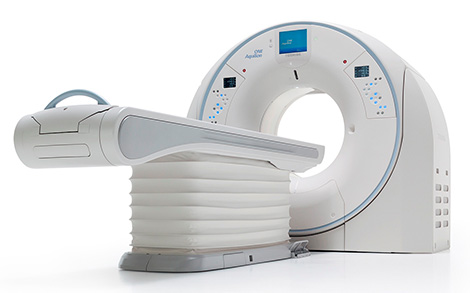
\includegraphics[bb=0.000000 0.000000 470.000000 293.000000,width=0.9\hsize]{image2/chapter1/toshibaCT.jpg} 
  \end{center}
  \vspace{-1cm}
  \caption*{}
 \end{minipage}
 \begin{minipage}{0.5\hsize}
  \begin{center}
 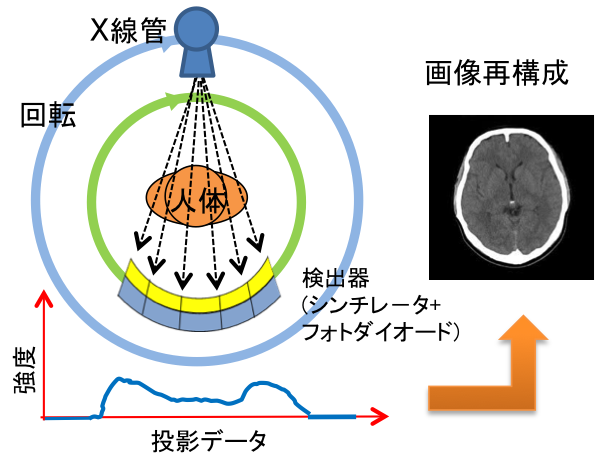
\includegraphics[bb=0.000000 0.000000 287.496234 222.221630,width=0.9\hsize]{image2/chapter1/CT_genri.png} 
  \end{center}
  \vspace{-1cm}
  \caption*{}
 \end{minipage}
 \begin{center}
  \caption{(左)X線CTの外観と(右)X線CTの原理\cite{toshiba_CT}}
  \label{fig:gaikan}
  \end{center}
\end{figure}


\section{従来のX線CTの問題点}
フォトダイオードの暗電流は 数十pA$\sim$数百pAであり、この暗電流に十分打ち克つ信号電流を検出器から出力する必要がある。CTの画質を律速しているのは「信号電流($I_s$)$\gg$暗電流($I_d$)」を実現することに他ならない。ここで従来のCTにおいて「$I_s\gg I_d$」を実現させるために必要な照射線量を概算してみる。被写体透過後のX線強度を$I_x$[/s]、PDの暗電流$I_d$を100[pA]とする。60keVのX線が従来一般的に用いられるGOSシンチレータ(40,000 ph/MeV)に検出されたとし、PDの量子効率を50\%すると、

\begin{align}
I_d&\gg I_s\\
60\times40\times0.5\times1.6\times10^{-19} [C] \times I_x&\gg100\times10^{-12}\\
I_x&\gg 5.2\times10^5
\end{align}
程度となる。また読み出し回路を通ることでさらにノイズが増大することを考えれば被写体を透過した時点で$10^{6}$cts/s/mm$^2$のレートが必要になる。人体透過後は線量は約1/1000になるので\footnote{人体を水と透過と考え60keVにおける水の線減弱係数は0.206[1/cm]、人体を30cmとすれば$e^{-\mu L}\sim1/1000$となる。}必要な照射線量は$10^{8-9}$cts/s/mm$^2$と膨大になる。このためX線CTによる医療被ばく量は膨大であり一回の撮影での被ばく量は10mSvにもおよびこれは成人の年間被ばく量の5倍に相当する\Fref{fig:dose}(左)。また日本においてはCTの普及率が世界1位であるため\Fref{fig:dose}(右)、国民一人あたりの医療被ばく量が諸外国に比べて圧倒的に高い。特に子どもや妊婦においては発がんリスクが高まることが報告されておりCTの適用が制限されている。日本においてはこれから高齢者人口が増えCTの需要はさらに高まり、このCTによる医療被ばくの問題は増々深刻化すると考えられる。

また超高線量下おいては様々なエネルギーの混ざった混合エネルギーのX線のそれぞれの反応パルスイベントを区別するのは困難であり、読み出し方法はある一定時間電荷を積分した電流モードである。そのため個々のX線光子のエネルギー情報は完全に失われてしまう。そのため得られる画像はCT値のみをパラメーターとしたモノクロ画像となってしまうため、CT値が同一の物質の弁別が困難であったり、ビームハードニングアーチファクトが発生してしまうのが二点目の問題である。このような背景から「低被ばく」かつ「多色」X線CTの必要性が高まっている。


\begin{figure}[H]
 \begin{minipage}{0.5\hsize}
  \begin{center}
 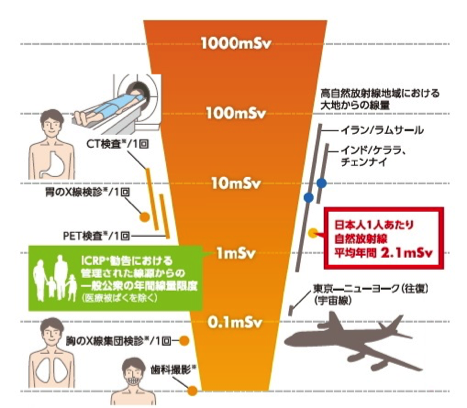
\includegraphics[bb=0.000000 0.000000 224.141471 195.823812,width=0.9\hsize]{image2/chapter1/dose_medical.png} 
  \end{center}
  \vspace{-1cm}
  \caption*{}
 \end{minipage}
 \begin{minipage}{0.5\hsize}
  \begin{center}
 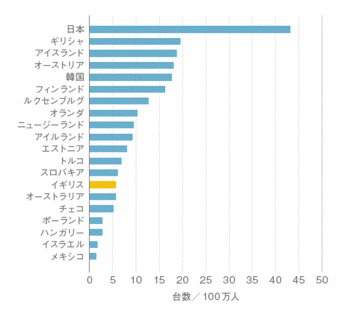
\includegraphics[bb=0.000000 0.000000 350.000000 313.000000,width=0.9\hsize]{image2/chapter1/CT_number.png} 
  \end{center}
  \vspace{-1cm}
  \caption*{}
 \end{minipage}
 \begin{center}
  \caption{(左)自然放射線と医療放射線の被ばく量比較(右)各国のCT保有台数\cite{dose}}
  \label{fig:dose}
  \end{center}
\end{figure}



\section{各医療メーカーの新型CT}
上述のように「低被ばく」かつ「多色」X線CTの必要性が高まる中でCTメーカー各社も様々な手法でそれを実現しようとしてる。GEにおいてはASiR-VというFBPとMLEMを組み合わせた新たな画像再構成アルゴリズムを開発し従来よりも低線量でも同等の画質を保てるCTを開発している。また、X線管を回転させながら高速で管電圧を80kVと140kVを切り替えることによってデュアルエナジーCTを実現している。またPhilipsにおいてはシンチレーターを二層式にすることで、一層目で低エネルギーのX線を検出し、二層目で高エネルギーのX線を検出することで2通りのCT画像を取得するデュアルエナジーCTを製品として出している。シーメンスは90度の角度差をつけた位置にX線管を配置し、管電圧を80kVと140kVのX線を照射することにより2色のデュアルエナジーCTを実現している。

\begin{figure}[H]
 \begin{center}
 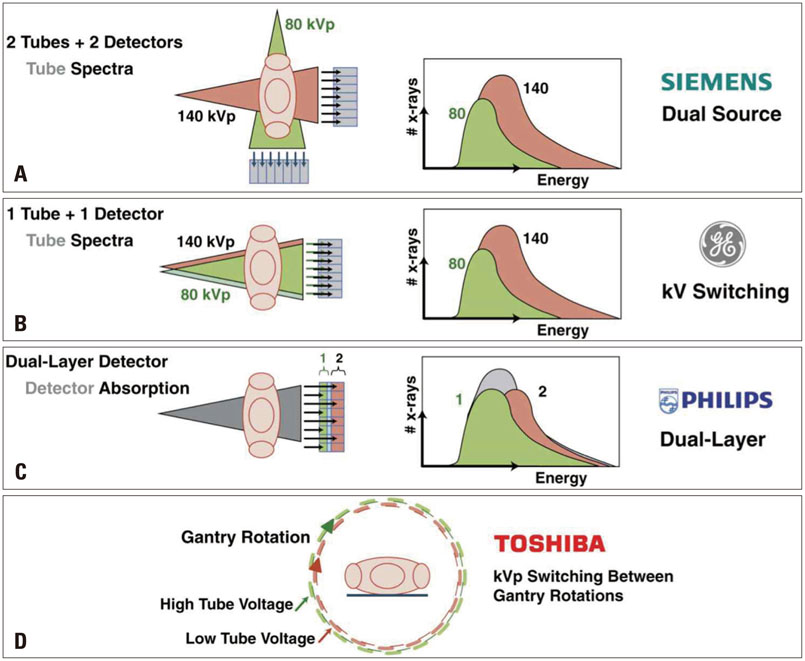
\includegraphics[bb=0.000000 0.000000 399.724138 328.220690,width=0.7\hsize]{image2/chapter1/CT_maker.jpg} 
 \end{center}
 \caption{各CTメーカーの製品化されているスペクトルCTの方式\cite{dualCT}}
 \label{fig:maker}
\end{figure}

しかし、新たな画像再構成法による低被ばく化は50\%程度にとどまり、多色化は2色にとどまっているのが現状である。

\section{本研究の目的と概要}
そこで、本研究では次世代光センサーMulti-Pixel Photon Counter (MPPC)と高速シンチレータを用いて、「低被ばく」かつ「多色」撮影が可能な、全く新しい革新的X線CTシステムを提案する。MPPCは100万倍以上の大きな内部増幅機能をもつ半導体光素子で、微弱信号への感度が極めて高く「信号電流$\gg$暗電流」の特性を持つ検出器である。この大きな内部増幅により、従来型CTより遥かに低い線量で同等以上のS/Nを実現し、一方ではエネルギー弁別による多色CTも実現可能になると期待され、X線CT誕生初期からの問題であった、「物質同定」や「ビーブハードニングアーチファクト低減」、さらには「K-edgeイメージング」など新たなイメージングも可能となり画像診断の幅を大きく広げることが期待される。さらに、比較的容易に既存のCT装置と置き換えが可能と見込まれ、臨床応用へのハードルを下げることができる。本研究では最初の実証試験を行った。
本論文では、まず第2章でX線の発生機構や物質との相互作用について述べ、第3章ではシンチレータと本実験で用いるフォトダイオード(PD)、アバランシェフォトダイオード(APD)、MPPCの性能や構造について述べる。第4章ではフォトンカウンティングCTの検出器として近年注目されている、直接検出型のCdTe検出器について述べ、その原理や構造と利点と欠点について述べる。第5章ではX線CTの構造や原理について詳細に述べ、上述した従来のX線CTの問題点について詳細に述べる。第6章では低被ばく化の検証実験として従来型のCTと、画像ノイズ(SD)、空間分解能、低コントラスト分解能をそれぞれ評価した結果について述べる。第7章では多色イメージングについて述べ、「ビームハードニングアーチファクト低減」、「物質同定」、「K-edgeイメージング」、「低コントラスト分解能向上」など従来のエネルギー積分型のCTでは実現的なかった多色イメージングについて述べる。最終8章ではまとめと今後の展望について触れたい。






	% 本文1

\chapter{X線の物理}
\section{X線の定義と発生}
X線は原子,特に核外から放出される電磁波,いわゆる光子線の一種である。その物理的性質は核内から放出される$\gamma$線と同じである。\\
\ \ X線は荷電粒子である電子を物質と衝突させることにより得られる。すなわち,電子のエネルギーが電磁放射線のエネルギーに転換した結果としてX線が発生する。\Fref{fig:Xray}(左)に放射線医学に広く用いられているクーリッジ管方式によるX線の発生原理を示す。陰極の一部にタングステン・フィラメントを封入し,これに約10V程度の加熱電圧をかけると白熱したフィラメントから熱電子が放出される。この熱電子を高電圧で加速し,X線管球の陽極に封入された金属ターゲットに衝突させることでX線が発生する。発生するX線には「制動放射線」と「特性X線」がありX線のスペクトルは様々なエネルギーのX線光子から成る,混合エネルギースペクトルとなる\Fref{fig:Xray}(右)。制動放射線は電子原子核近傍を通るとき,原子核の電場によって曲げられ,失った運動エネルギーとして放出される。特性X線は電子が軌道電子に衝突し,軌道電子が電離されると,できた空席にそれより高いエネルギー順位の軌道電子が落ち込むときに発生する。制動放射線はターゲットの元素には依存しないが,特性X線はターゲットによって異なる。発生したX線には透過性が低いX線も含まれるので,被写体を透過し得ないX線をあらかじめ取り除くために,射出窓には濾過版(フィルター)が設けられている。\\
\ \ X線のスペクトルは陰極,陽極管の加速電圧(管電圧),X線管に流れる電流(管電流)によってきまり,管電圧を上げることでX線のエネルギーが高くなり,管電流を上げることでX線強度が上がる。
\  \ 混合エネルギースペクトルのX線質を表す量として実効エネルギーがある。実効エネルギーとは,連続エネルギー分布を持ったX線の半価層が単色X線の半価層\footnote{制動放射線の50$\%$透過率の厚さで定義される}と等しい時,その単色X線のエネルギーのことを実効エネルギーとして使用する。

\begin{figure}[H]
 \begin{center}
 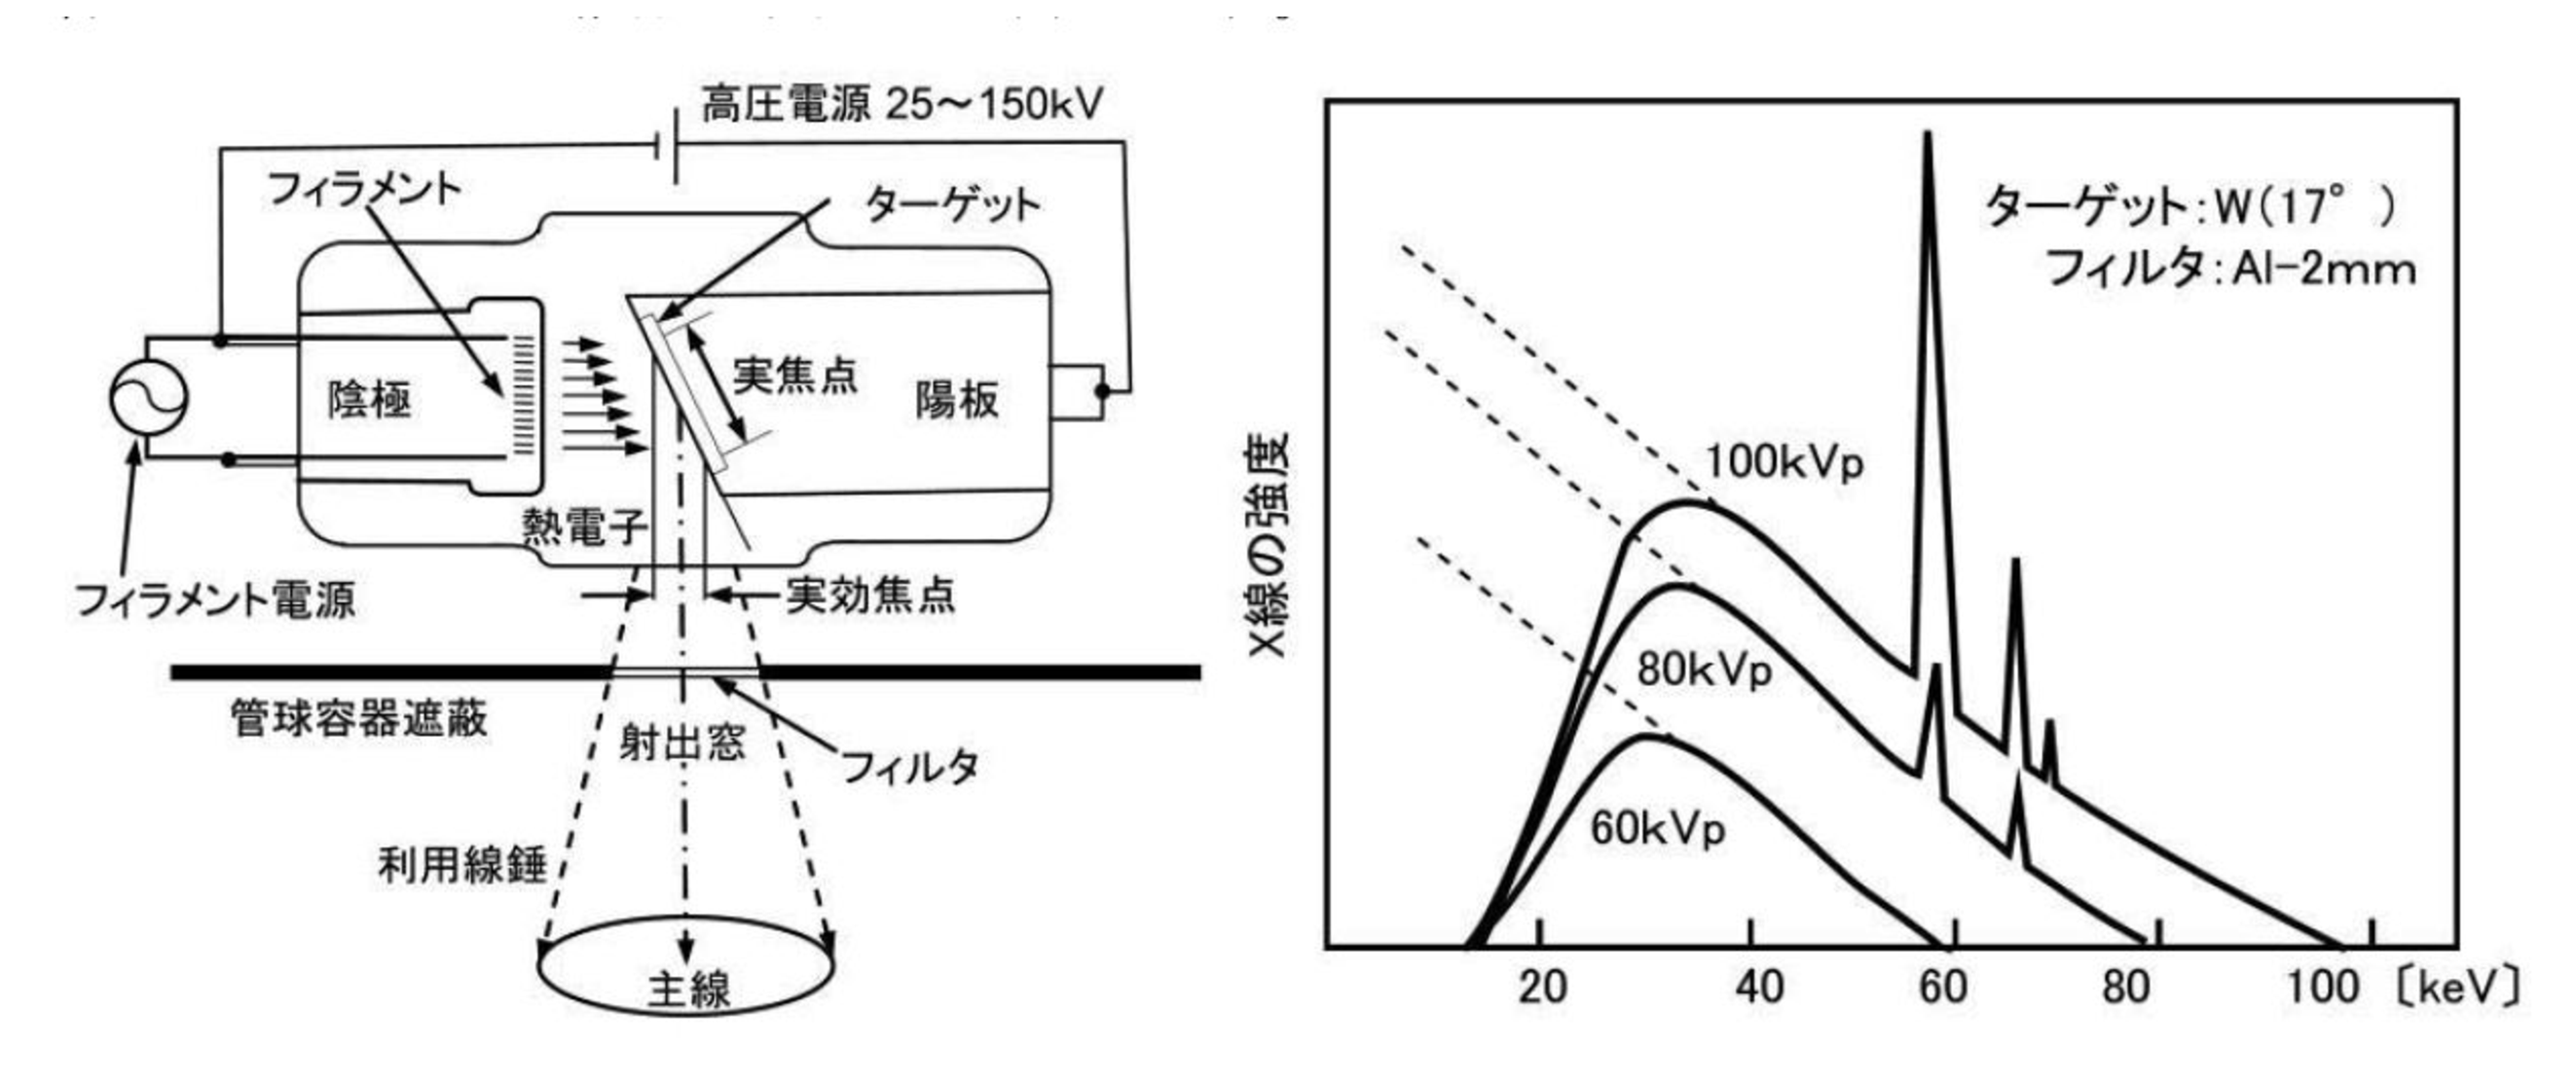
\includegraphics[width=14cm]{image/other/X-ray.eps}
 \end{center}
 \caption{X線管の構造(左)とX線スペクトル(右)\cite{iinuma}}
 \label{fig:Xray}
\end{figure}

%
\if0

\subsection{$\gamma$線の定義と発生}
$\gamma$線は励起した原子核が低いエネルギー準位へ遷移する際に放出されるる電磁放射線である。本実験で用いる$\gamma$線線源の特性を\Tref{RI}に示す。

\begin{table}[H]
\begin{center}
\begin{tabular}{|l|l|l|l|l|} \hline
\multicolumn{1}{|c|}{核種} & \multicolumn{1}{c|}{半減期} & \multicolumn{1}{c|}{崩壊形式} &\parbox{12zw}{主な$\beta$線(または$\alpha$線)のエネルギーと放出の割合} & \parbox{10zw}{主な$\gamma$線のエネルギーと放出割合} \\\hline
$^{57}$Co & 271.8d & EC & 100$\%$ & 0.0144(10\%) \\
 &  &  &  & 0.122(86\%) \\
 &  &  &  & 0.136(10\%) \\
 &  &  &  & 0.0064 Fe-X \\\hline
$^{60}$Co & 5.270y & $\beta^{-}$ & 0.318(100\%) & 1.173(100\%) \\
 &  &  &  & 1.333(100\%) \\\hline
$^{109}$Cd & 463d & EC & 100\% & 0.0222\ Ag-X \\\cline{2-5}
$^{109m}$Ag & 39.6s & IT & 100\% & 0.0880(3.6\%) \\
 &  &  &  & 0.0222\ Ag-X \\\hline
$^{133}$Ba & 10.5y & EC & 100\% & 0.0810(34\%) \\
 &  &  &  & 0.276(7.2\%) \\
 &  &  &  & 0.303(18\%) \\
 &  &  &  & 0.356(62\%) \\
 &  &  &  & 0.384(8.9\%) \\
 &  &  &  & 他 \\
 &  &  &  & 0.0310\ Cs-X \\\hline
$^{241}$Am & 432.2y & $\alpha$ & 5.388(1\%) & 0.0263(2.4\%) \\
 &  &  & 5.443(13\%) & 0.0595(36\%) \\
 &  &  & 5.486(85\%) & 他 \\
 &  &  & 他 & 0.0139\ Np-LX \\\hline
\end{tabular}
\end{center}
\caption{本実験で使用する$\gamma$線線源\cite{RI}}
\label{RI}
\end{table}

\fi
%

\section{X線の物質との相互作用}
X線の物質との相互作用には光電吸収,コンプトン散乱,電子対生成がある。
\subsection{光電吸収}

\begin{figure}[H]
 \begin{center}
 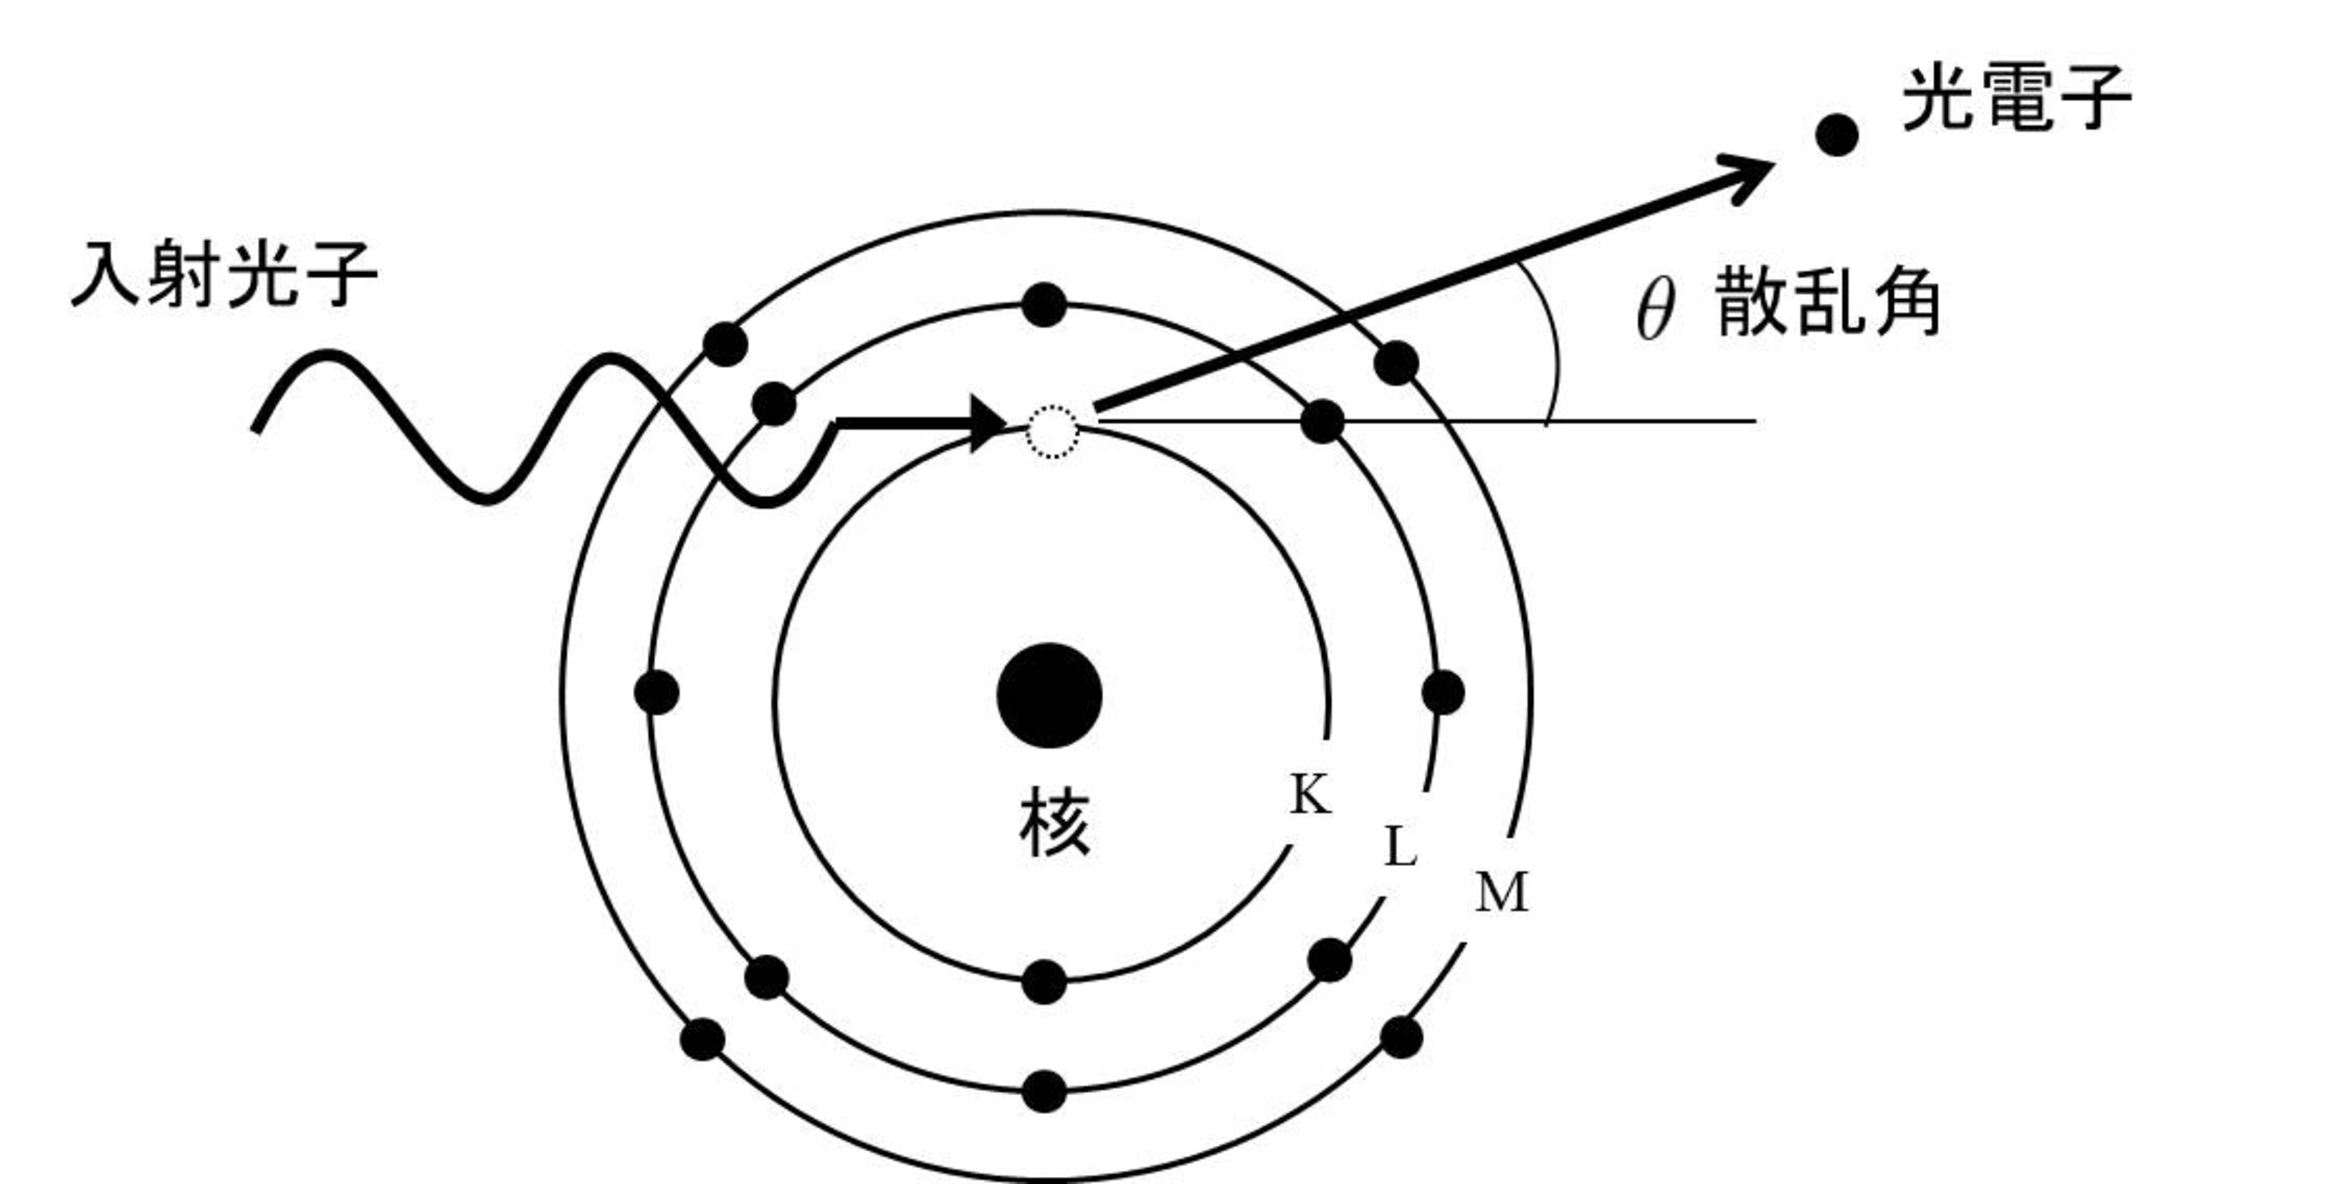
\includegraphics[width=10cm]{image/other/photo_ab.eps}
 \end{center}
 \caption{光電吸収}
 \label{fig:photo_ab}
\end{figure}

光電効果とは,物質に入射した光子が物質の軌道電子に当たり,そのエネルギーを全てその軌道電子に与え,入射した光子は消滅し軌道電子はその原子の外側へ飛び出す現象である。この原子から飛び出した軌道電子のことを光電子と呼ぶ。このとき軌道電子が原子の外に放出され,その空位の軌道を埋めるために外側の軌道電子が落ち込み,軌道電子の結合エネルギー差に相当する1個あるいはそれ以上の特性X線が放出される。いくらかの割合\footnote{放出された特性X線の光子数と光電吸収によって吸収された光子数の比を蛍光収率$\omega$といい,オージェ電子放出の割合をオージェ収率といい$(1-\omega)$で表される。K殻における蛍光収率は原子番号が高いほど高くなり,例えば$Z=75$においてはK殻において起きた光電吸収のうち93$\%$から特性X線が生じ,7$\%$からオージェ電子が生じる。逆に原子番号の低い物質の場合,蛍光収率は下がり,オージュエ収率が高くなる。}でこの結合エネルギーの差は特性X線の代わりにL殻よりゆるい結合である外側の殻から軌道電子を原子外に放出する場合がある。この電子をオージェ電子という。すなわち,軌道電子に与えられた光子のエネルギーは,最終的には光電子および付随して発生する特性X線またはオージェ電子の形でその原子の外へ放出される。\Fref{fig:photo_ab}に光電吸収の相互作用の過程を示す。光電子が受け取るエネルギー$E$は入射光子のエネルギーを$h\nu$,軌道電子の結合エネルギーを$I$とすると
\begin{align}
E=h\nu-I \label{eq:kou_ele}
\end{align}
で示される。つまり,入射光子のエネルギーは軌道電子の結合エネルギー$I$以上のエネルギーを持っている必要があり,これより光子エネルギーが小さい場合には光電吸収は起こらない。また,光電吸収は光子のエネルギーが大きすぎて,軌道電子に完全に吸収されない場合にも起こらない。1個の原子あたりの光電吸収の反応断面積$\sigma_{\rm photo}$は粗い近似式として,入射光子のエネルギー$E$,物質の原子番号を$Z$として
\begin{align}
\sigma_{\rm{photo}}\propto\frac{Z^{4-5}}{E^{3.5}} \label{eq:sigma_photo}
\end{align}
と表され,光電吸収が起きる確率は入射光子のエネルギーが低エネルギーかつ,原子番号が高い物質ほど増大する。逆に,入射光子のエネルギーが高いほど激減するため,光電吸収は高エネルギー領域では無視できる程小さくなる。しかし,鉛のように原子番号が高い元素では無視できなくなる。\\
\ \ また,光電吸収はK殻において最も起こりやすく,約80$\%$の光電吸収ががK殻で起きることが実験的に確かめられているが\footnote{K殻の軌道電子の束縛エネルギーが最も大きため,光電吸収はK殻において最も起きにくいように思われるがそれは誤りである。L殻やM殻などでは束縛エネルギーが小さいので,\Eref{eq:kou_ele}より原子から飛び出す光電子の速度が速くなるため,運動量も大きくなる。しかし,入射光子の運動量は極めて小さいため,入射光子と光電子の2体だけでは運動量保存則を満たことができず,第3体として原子核自体が反跳運動量を受け取る必要がある。したがって光電子の運動量が大きくなる,つまり束縛エネルギーが小さいほど運動量保存則を満たすことが困難となるため,束縛エネルギーの最も大きいK殻において光電吸収は最も起こりやすくなる。},L殻,M殻においても起きる。そのため入射光子のエネルギーがK殻,L殻,M殻結合エネルギーに等しくなるたびに急激に増大し不連続になる。この不連続部分を吸収端と呼ぶ。その結果,光電吸収断面積$\sigma_{\rm photo}$はジグザグを繰り返しながらエネルギーの増加とともに減少していく。

\subsection{コンプトン散乱}
入射光子のエネルギーが軌道電子の束縛エネルギーを無視できるほどになるとコンプトン散乱が起きるようになる。コンプトン散乱とは,入射光子が原子の軌道電子と衝突して,電子にエネルギーの一部を与えて弾き飛ばし,同時に入射光子自身はその分だけエネルギーを失って,波長が長くなり別の方向へ散乱される現象である(\Fref{fig:comp_geo})。弾き飛ばされた電子を反跳電子,散乱された光子を散乱光子と呼ぶ。

\begin{figure}[H]
 \begin{center}
 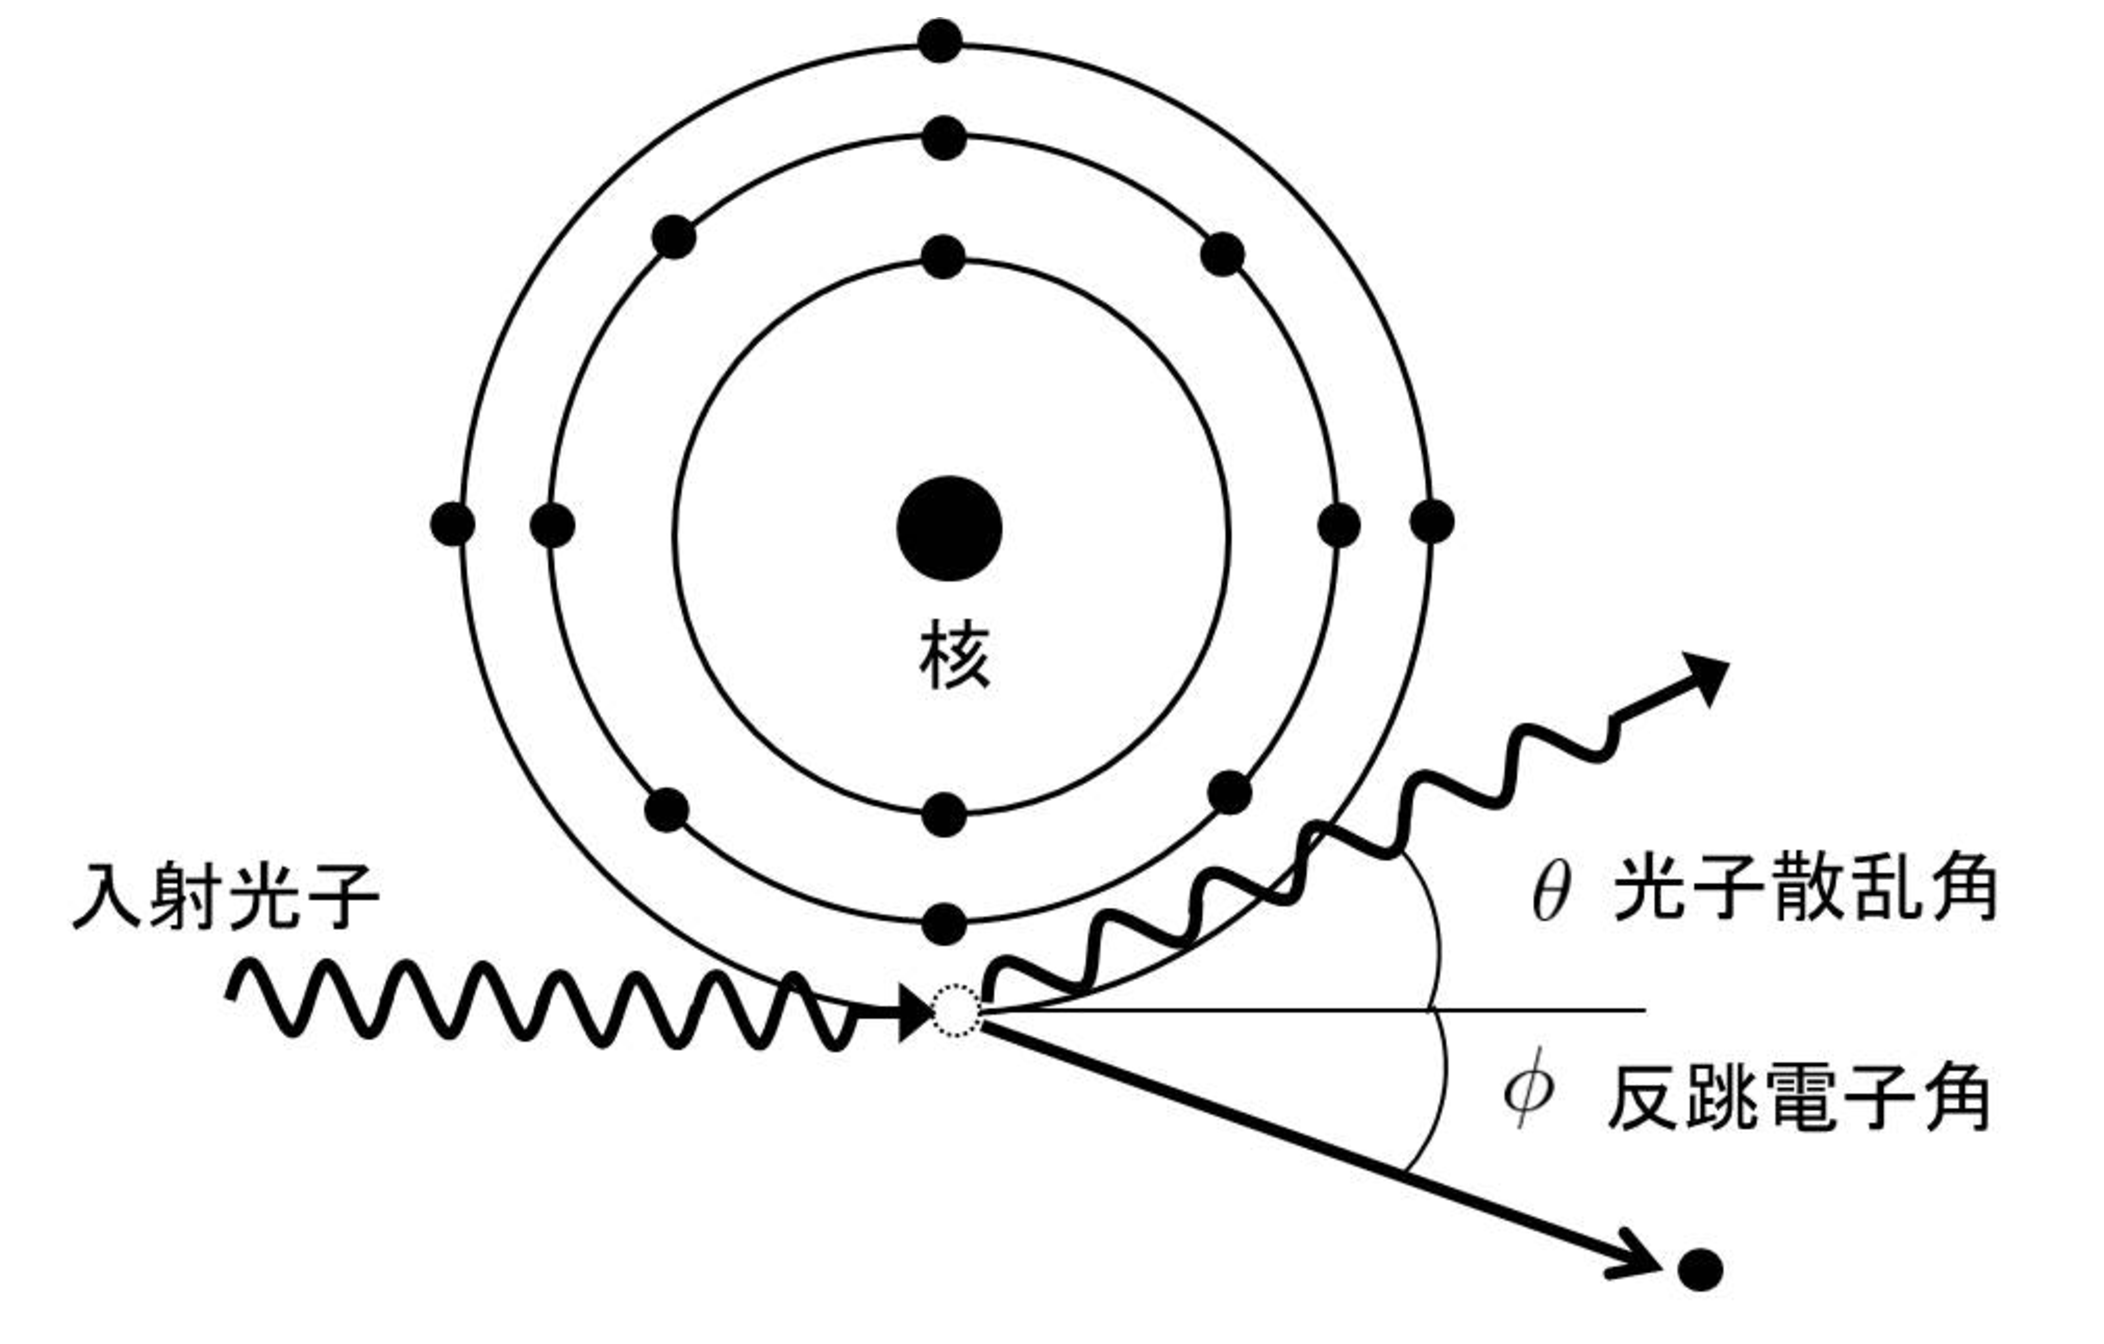
\includegraphics[width=10cm]{image/other/compton.eps}
 \end{center}
 \caption{コンプトン散乱}
 \label{fig:comp_geo}
\end{figure}

散乱光子のエネルギー$h\nu^{\prime}$はエネルギー保存則,運動量保存則より
\begin{align}
h\nu^{\prime}=\frac{h\nu}{1+\displaystyle\frac{h\nu}{m_oc^2}(1-\cos{\theta})} \label{eq:comp1}
\end{align}
と書くことができる。ここで$m_0c^2$は電子の静止質量エネルギー(0.511MeV)である。一方で反跳電子のエネルギー$E_r$は入射光子のエネルギーから,散乱線のエネルギーを差し引くだけなので,次式から容易に求めることができる。
\begin{align}
E_r=h\nu-h\nu^{\prime}=h\nu\left\{1-\frac{1}{1+\displaystyle\frac{h\nu}{m_0c^2}(1-\cos{\theta})}\right\} \label{eq:comp2}
\end{align}
\Eref{eq:comp2}より$\cos{\theta=1}$つまり$\theta=0^{\circ}$,すなわち散乱線が入射光子の入射方向と同じ方向に散乱されるとき$E_r=0$であり,エネルギーは反跳電子に伝達されず$h\nu^{\prime}=h\nu$となり,コンプトン散乱は起こらなかったことになる。一方で$\cos{\theta=-1}$つまり$\theta=180^{\circ}$,すなわち散乱線が入射光子の入射方向と反対方向に散乱されるとき$E_r$は最大となり
\begin{align}
E_{r\ \rm max}=h\nu\cdot\frac{1}{1+\displaystyle\frac{m_0c^2}{2h\nu}} \label{eq:comp_edge}
\end{align}
となる。このときの$E_{r\ \rm max}$とコンプトンエッジという。このとき,散乱線のエネルギーは最小となり\Eref{eq:comp1}より,
\begin{align}
h\nu^{\prime}_{\rm min}=\frac{h\nu}{1+\displaystyle\frac{2h\nu}{m_0c^2}} \label{eq:nyu_min}
\end{align}
となる。反跳電子のエネルギースペクトルは$E_r=0からE_{r\ \rm max}$まで分布し,連続スペクトルとなる。\\
\ \ 入射光子のエネルギーが比較的低いとき($h\nu\ll m_0c^2$),高いとき($h\nu\gg m_0c^2$)の散乱線の振る舞いを考える。まず入射光子のエネルギーが比較的低いときは,散乱線のエネルギーは\Eref{eq:comp1}より角度によらず$h\nu^{\prime}\fallingdotseq h\nu$で$E_r\fallingdotseq0$となり,これは入射光子が微小角だけ散乱され進行方向が変わるだけのトムソン散乱である。一方で入射光子のエネルギーが比較的高いときは$h\nu^{\prime}\fallingdotseq m_0c^2/(1-\cos{\theta})$となる。従って,$\theta=90^{\circ}$方向の散乱線のエネルギーは入射光子のエネルギーに関係なく0.51MeVとなり,$\theta=180^{\circ}$方向の散乱線のエネルギーはその半分の0.26MeVになる。\\
\ \ 散乱線の角度分布は角度$\theta$方向の微小立体角$d\Omega$に対する微分散乱断面積で表せる。それはクライン-仁科の式より以下で与えられる。
\begin{align}
\frac{\sigma_{\rm comp}}{d\Omega}=Z\cdot\frac{r_0^2}{2}(1+\cos^2{\theta})\cdot\left[\frac{1}{1+\alpha(1-\cos{\theta})}\right]^2\cdot\left[1+\frac{\alpha^2(1-\cos{\theta})^2}{(1+\cos^2{\theta})\{1+\alpha(1-\cos{\theta})\}}\right]
\end{align}
ここで$\alpha=h\nu/m_0c^2,r_0$は古典的電子半径であるこの分布は\Fref{fig:comp_sigma}に示すようになり,入射光子のエネルギーが高くなるにつれてコンプトン散乱の断面積は小さくなるが,前方散乱の割合が増大する。1個の原子あたりのコンプトン散乱の反応断面積$\sigma_{\rm comp}$は
\begin{align}
\sigma_{\rm comp}\propto\frac{Z}{E}\label{eq:sigma_comp}
\end{align}
と書ける。X線撮像に用いるエネルギー領域(40keV-140keV程度)ではコンプトン散乱は原子番号のみに依存する。

\begin{figure}[H]
 \begin{center}
 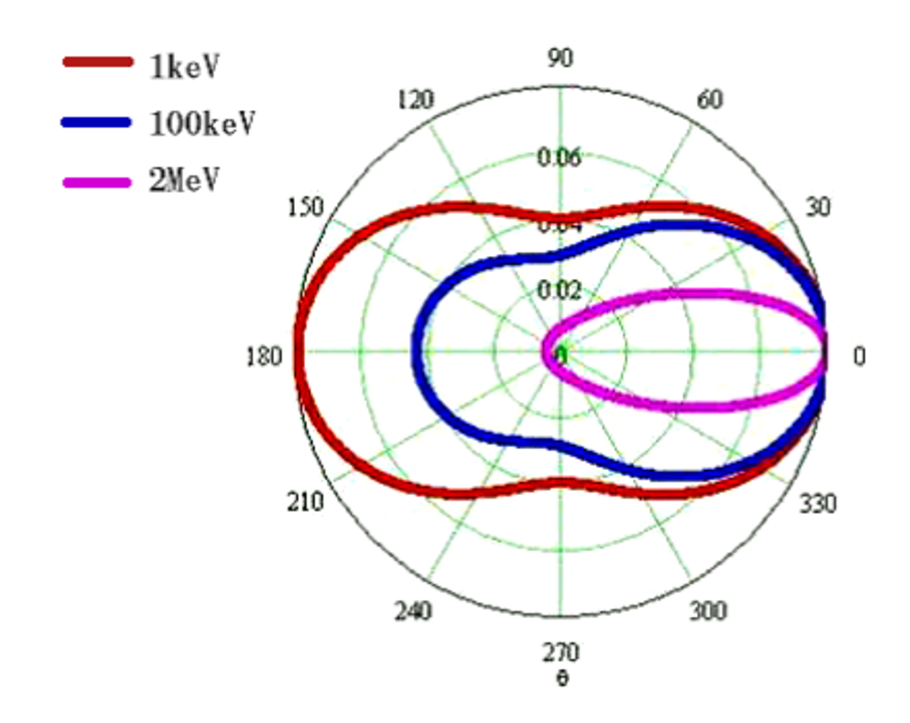
\includegraphics[width=10cm]{image/other/comp_cross.eps}
 \end{center}
 \caption{コンプトン散乱光子の角度分布\cite{nishidai}}
 \label{fig:comp_sigma}
\end{figure}

%
\if0
\subsection{電子$\cdot$陽電子対生成}
入射光子のエネルギーが電子の静止質量エネルギーの2倍すなわち,1.02MeVを越えると,コンプトン散乱は起こりにくくなるが電子対生成が起きるようになる。電子対生成とは1.02MeV以上の入射光子が原子の近くを通る際に,原子核のクーロン電場の中で光子が消滅し,代わって一対の電子と陽電子が生成される現象である(\Fref{fig:pair})。

\begin{figure}[H]
 \begin{center}
 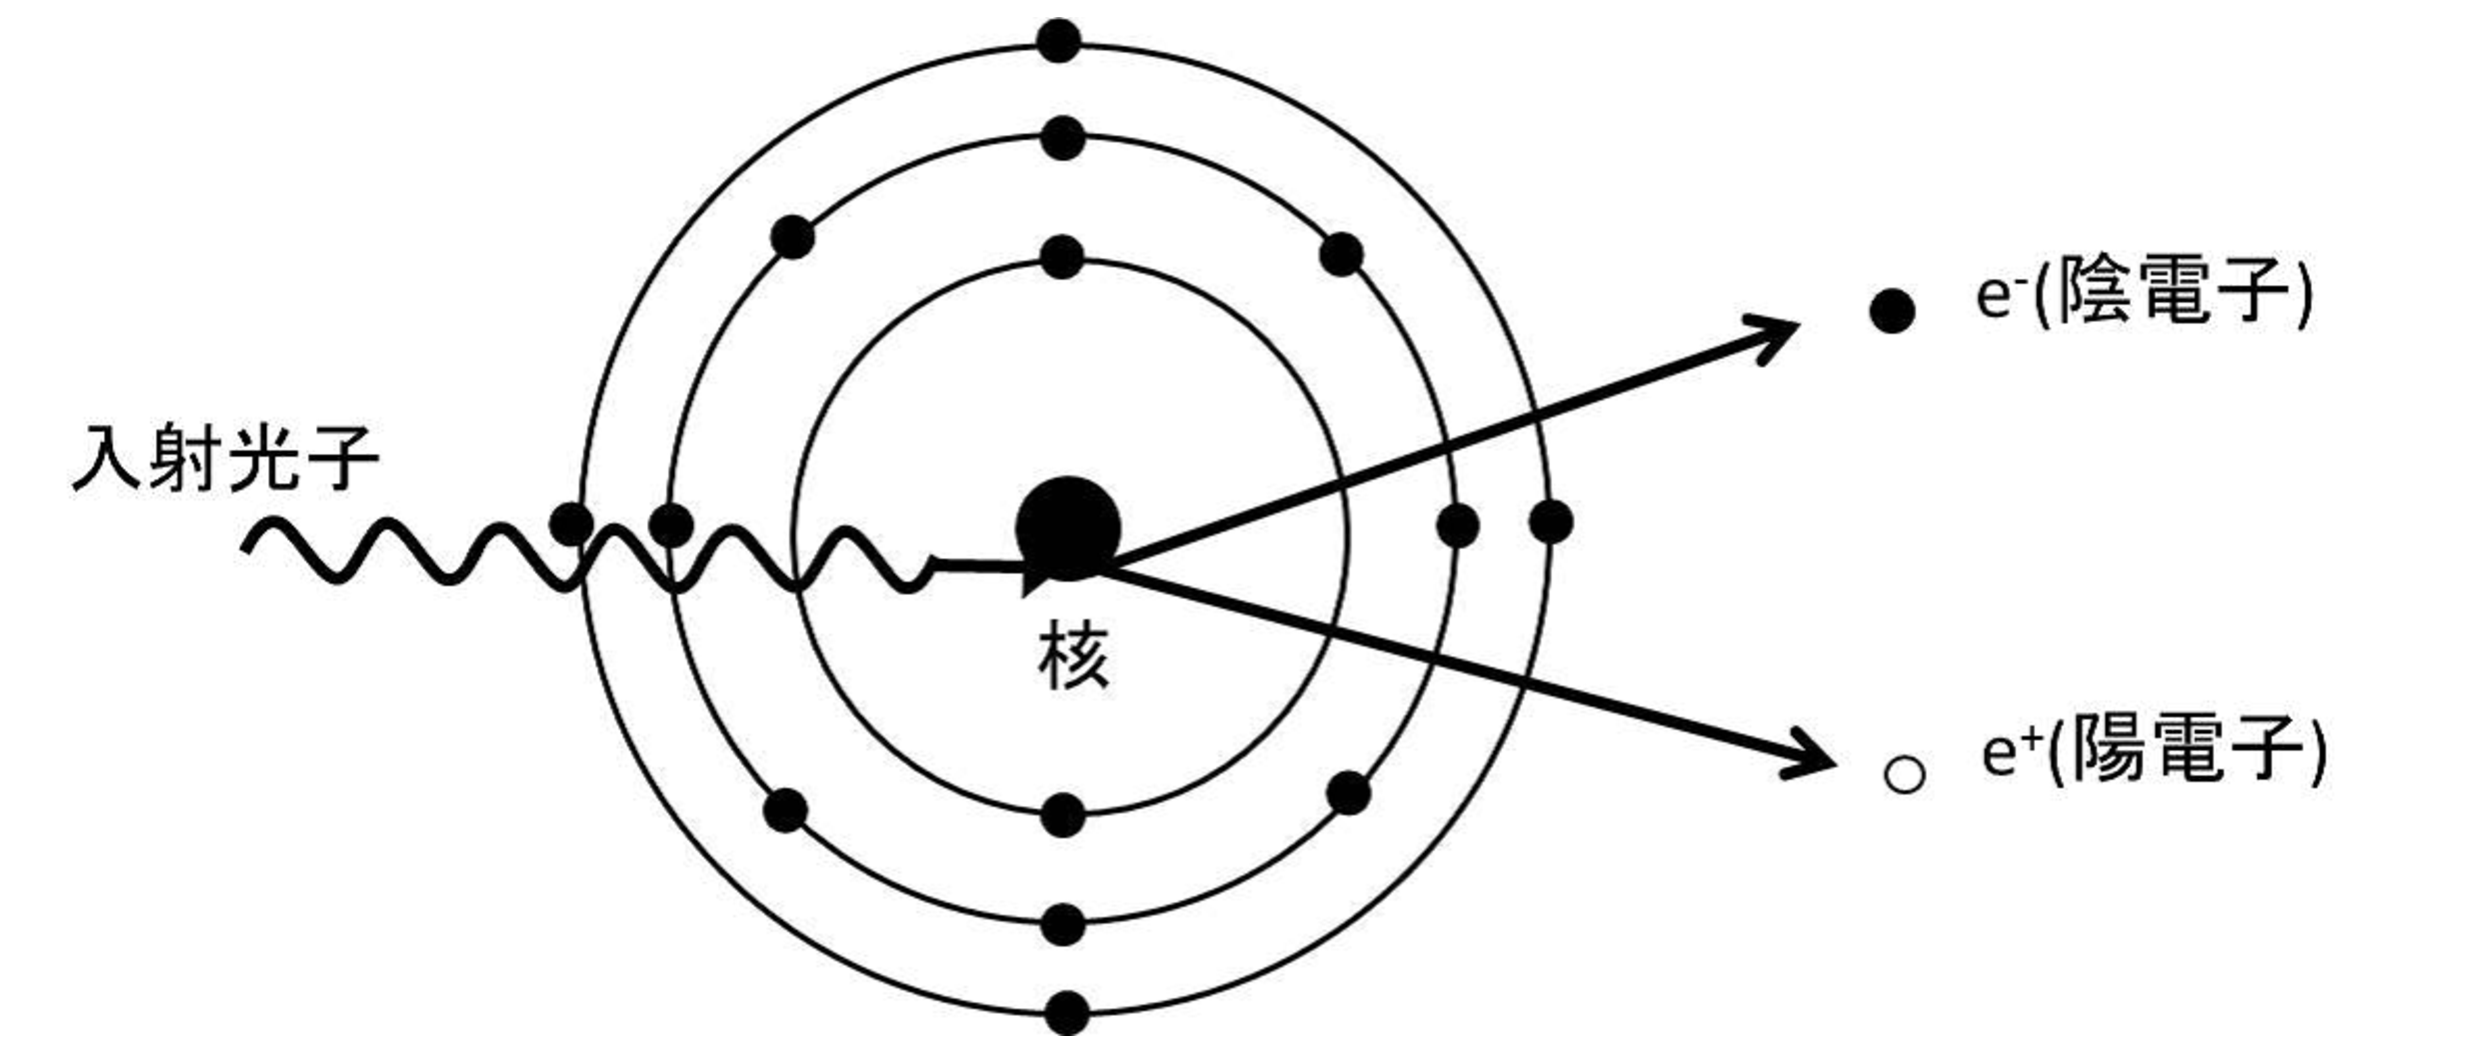
\includegraphics[width=10cm]{image/other/pair_create.eps}
 \end{center}
 \caption{電子対生成}
 \label{fig:pair}
\end{figure}


入射光子のエネルギーを$h\nu$,電子の静止質量エネルギーを$m_0c^2$,電子対生成によって生じた両電子の運動エネルギーを$E_+,E_-$とすると,エネルギーと質量の両保存則から次式が成り立つ。
\begin{align}
E_++E_-=h\nu-2m_0c^2 \label{eq:pair}
\end{align}
この式からわかるように,電子対生成では,入射光子のエネルギーの一部が両電子の質量静止エネルギーに転化し,残りがその運動エネルギーとなる。従って,電子対生成は入射光子のエネルギーが電子対の質量静止エネルギー1.02MeV($2m_0c^2$)より高くないと起こらない。また,電子対生成で生じた両電子の運動エネルギーは必ずしも等分配されず,$0からh\nu-2m_0c^2$まで広範囲にわたって分布する。1原子あたりの電子対生成の反応断面積$\sigma_{\rm pair}$は
\begin{align}
\sigma_{\rm pair}=Z^2(E-1.02) \label{eq:sigma_pair}
\end{align}
で表される。この式からわかるように,電子対生成は入射光子のエネルギーが高く,物質の原子番号が高いほど起こりやすい。

%
\fi

\section{X線の減弱\label{sec:atten}}

\begin{figure}[H]
 \begin{center}
 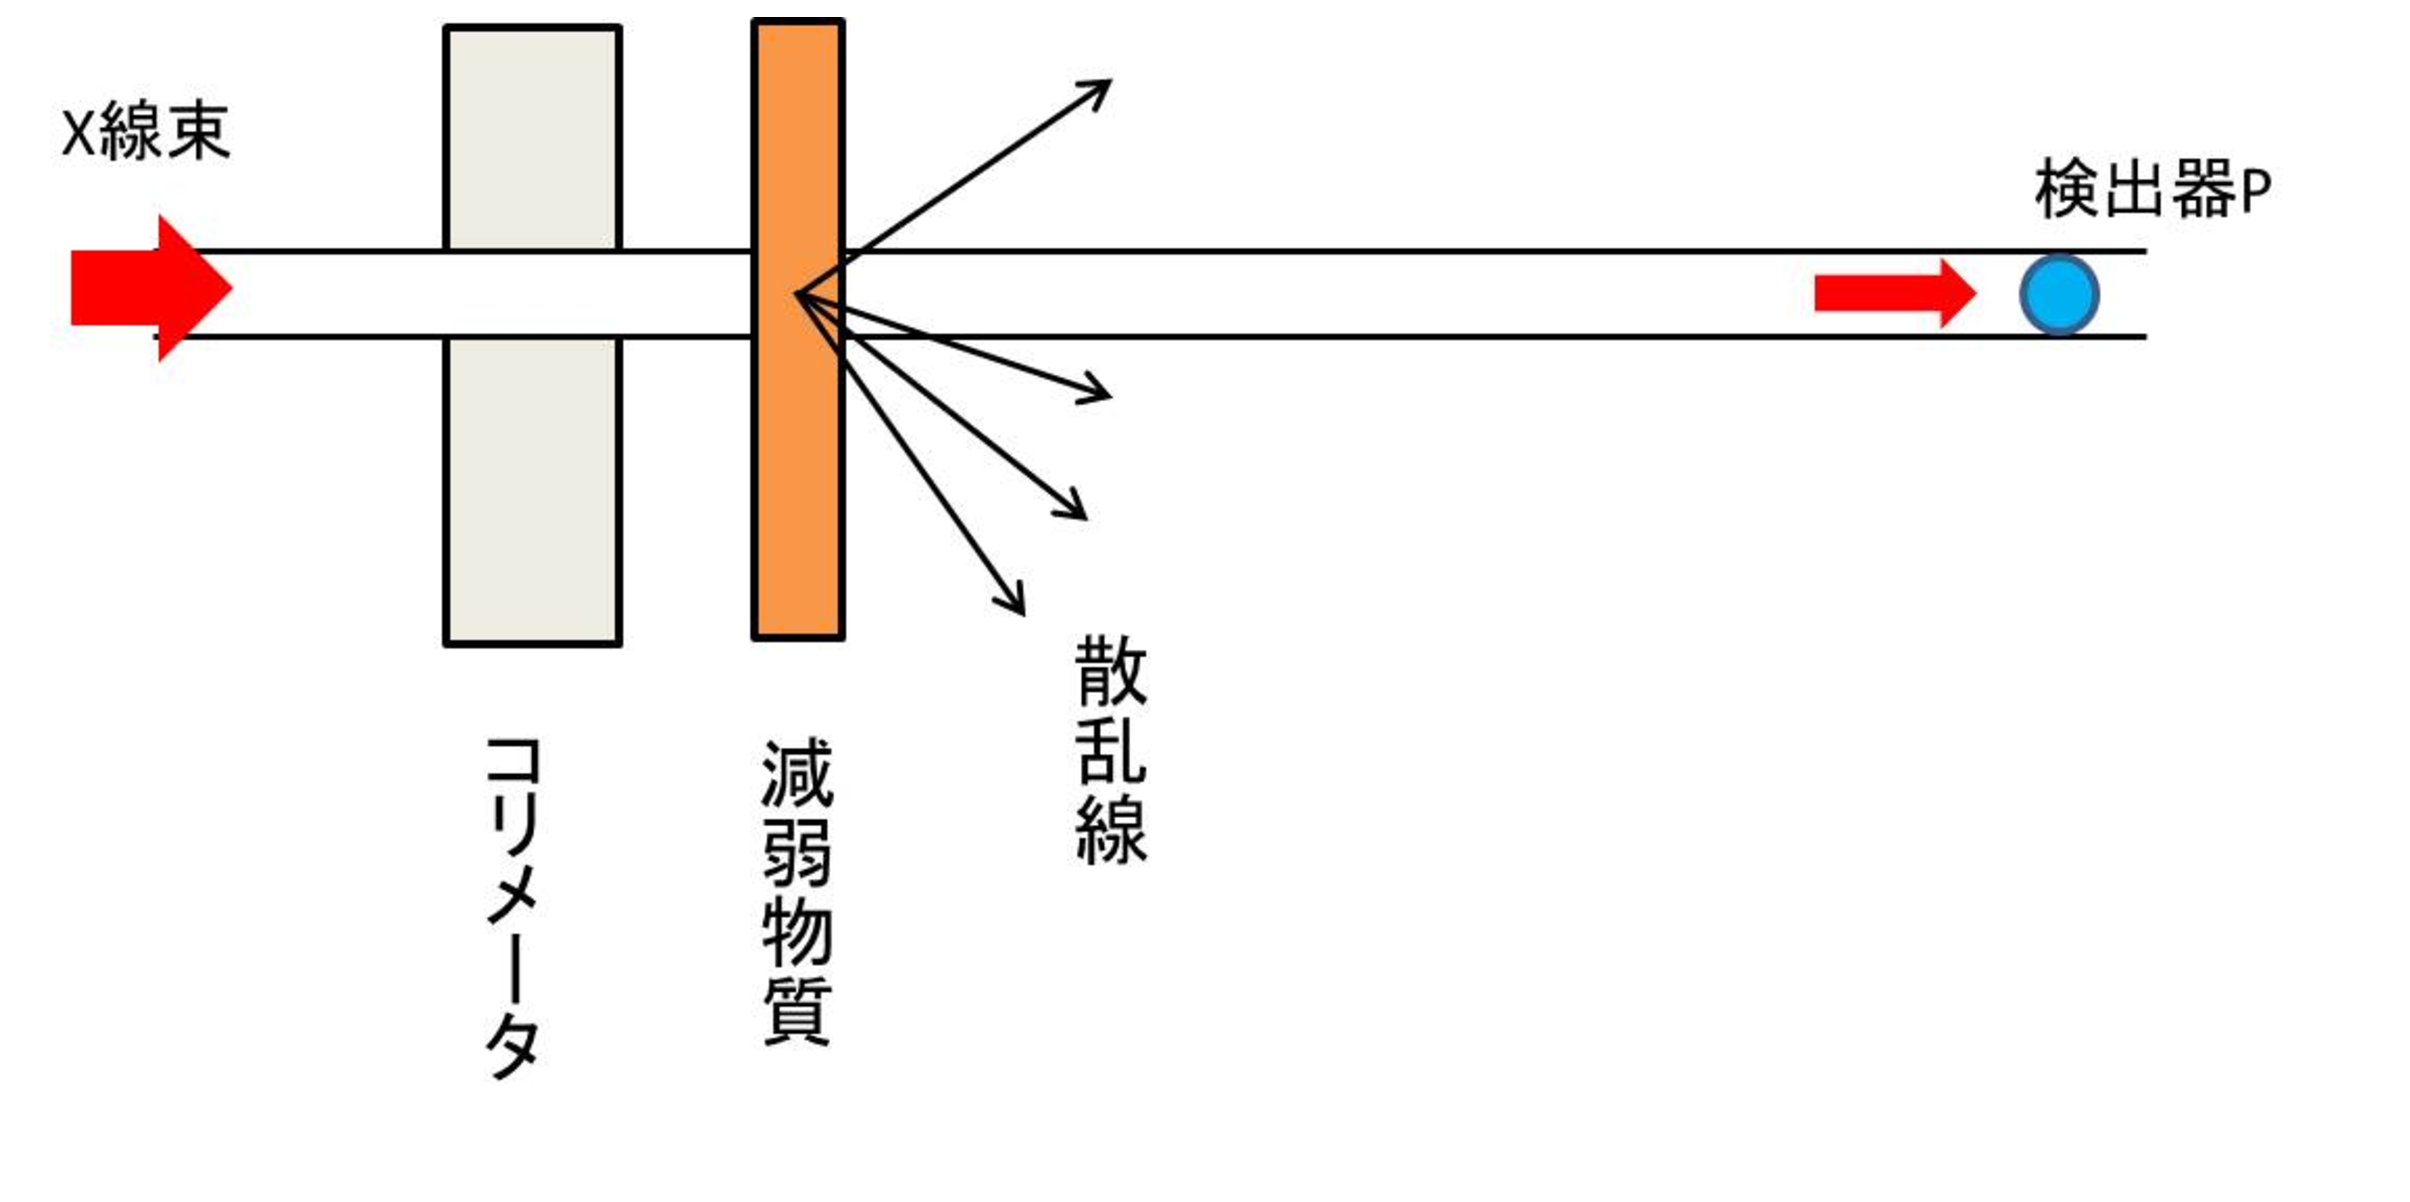
\includegraphics[width=10cm]{image/other/trans.eps}
 \end{center}
 \vspace{-1cm}
 \caption{X線束の物質による減弱測定}
 \label{fig:trans}
\end{figure}

\Fref{fig:trans}のような透過実験を想定し,この図で単一エネルギーのX線束(単色X線)あるいは$\gamma$線の物質中での減弱について考える。物質と全く相互作用を起こさず,X線束上の検出器Pに到達する透過光子数を求める。この場合,一度でも物質と相互作用をした散乱線はその進行方向が変わり,検出器Pに到達することができない。検出器Pに到達する透過光子数$I$は入射光子数と$I_0$,物質の厚さを$x$として
\begin{align}
I=I_0e^{-\mu x} \label{eq:atten}
\end{align}
と表せる。ここで$\mu$は線源弱係数であり単位は[1/cm]である。これは物質厚さ$x$を厚くすると指数関数的に減衰していく。\\
\ \ 本来,物質のある点において,ある光子が相互作用を起こすがどうかは全くの確率現象であり,その確率はポアソン分布に従うものである。すなわち\Eref{eq:atten}の$e^{-\mu x}$は光子が相互作用を起こさずに物質中を通過する確率を巨視(マクロ)的に表しており,その確率は主に光電吸収,コンプトン散乱,電子対生成の微視(ミクロ)的な相互作用による確率の積である。すなわち,
物質構成原子の1個あたりの全断面積$\sigma$
\begin{align}
\sigma=\sigma_{\rm photo}+\sigma_{\rm comp}+\sigma_{\rm pair} \label{eq:sigma_all}
\end{align}
に比例した値になる。各断面積は\Eref{eq:sigma_photo},\Eref{eq:sigma_comp},\Eref{eq:sigma_pair}で示した通り,
\begin{align}
\begin{cases}
\sigma_{\rm photo}\propto Z^{4-5}/E^{3.5}\\
\sigma_{\rm comp}\propto Z/E\\
\sigma_{\rm pair}\propto Z^2(E-1.02)
\end{cases}
\end{align}
である。したがって原子1個あたりの全断面積$\sigma$は原子番号$Z$と入射エネルギー$E$の複雑な関数となる。物質の単位体積あたりの原子数を$n$とすると,線源弱係数$\mu$は
\begin{align}
\mu&=n\sigma \\
&=n\sigma_{\rm photo}+n\sigma_{\rm comp}+n\sigma_{\rm pair}\\
&=\mu_{\rm photo}+\mu_{\rm comp}+\mu_{\rm pair}
\end{align}
となり,線減弱係数はそれぞれの相互作用における線減弱係数の和として表すことができる。\\
\ \ 線源弱係数$\mu$は同じ物質であってもその密度に依存して変化するために,一般に線源弱係数$\mu[\rm cm^{-1}]$を物質の密度$\rho[\rm g/cm^{3}]$で割った値が用いられる。これを質量減弱係数といい$\mu_m[\rm cm^2/g]$で表す。アボガドロ数を$N_A$,原子量を$A$とすると,1gあたりの原子数$n/\rho=N_A/A$なので%アボガドロ数個の原子の個数分の重さが原子量
\begin{align}
\mu_m=\frac{\mu}{\rho}=\frac{n\sigma}{\rho}=\frac{N_A}{A}\sigma \label{eq:mass_atten}
\end{align}
となる。この式から$\mu_m$は物質の密度には関係せず,原子番号と入射光子のエネルギーのみに依存することがわかる。線源弱係数は同じ物質であってもその密度によって依存する,また物質が異なっても密度によっては同一になる場合があるが,質量減弱係数は物質に固有な値なので,線源弱係数より便利である。\\


\ \ \Fref{fig:mass_atten}は一例として,NaI(Tl)の線減弱係数$\mu$とそれを構成する光電吸収,コンプトン散乱,電子対生成のそれぞれの線減弱係数が入射光子のエネルギーによってどのように変化するかを示したものであり,\Fref{fig:mu_dist}は入射光子エネルギーと光電吸収,コンプトン散乱,電子対生成の各相互作用の優勢領域を示したものである。

\begin{figure}[H]
 \begin{center}
 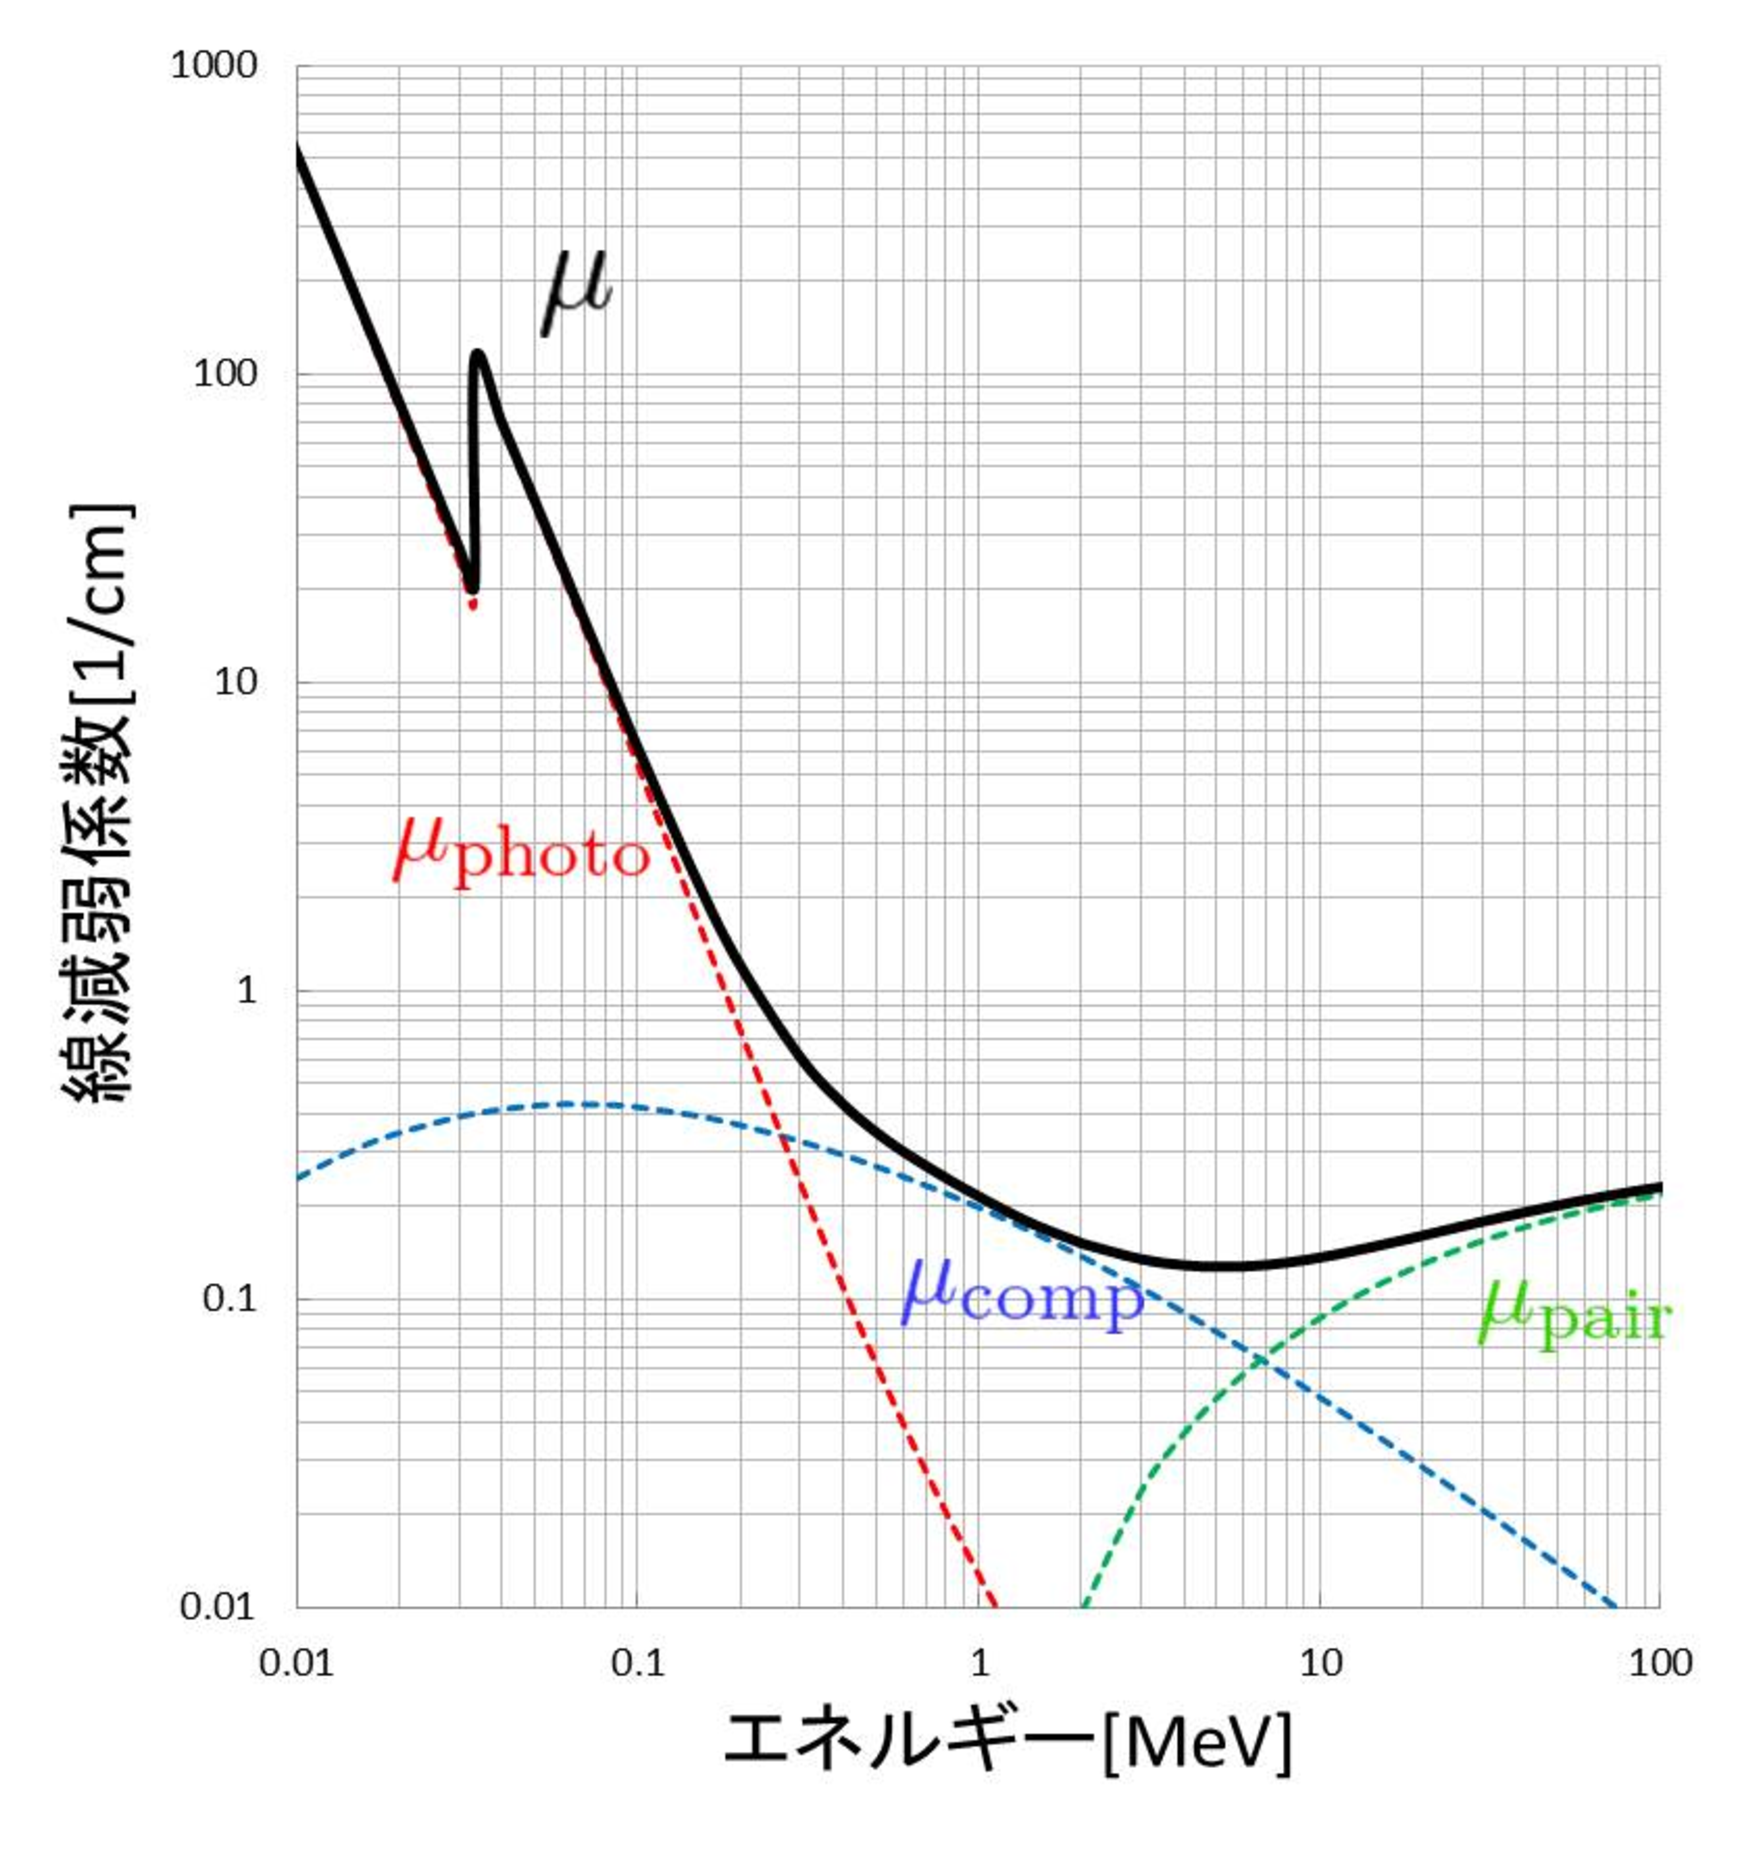
\includegraphics[width=8cm]{image/other/NaI_mu.eps}
 \end{center}
 \caption{NaI(Tl)の線減弱係数とその成分[NIST\cite{nist}より作成]}
 \label{fig:mass_atten}
\end{figure}

\begin{figure}[H]
 \begin{center}
 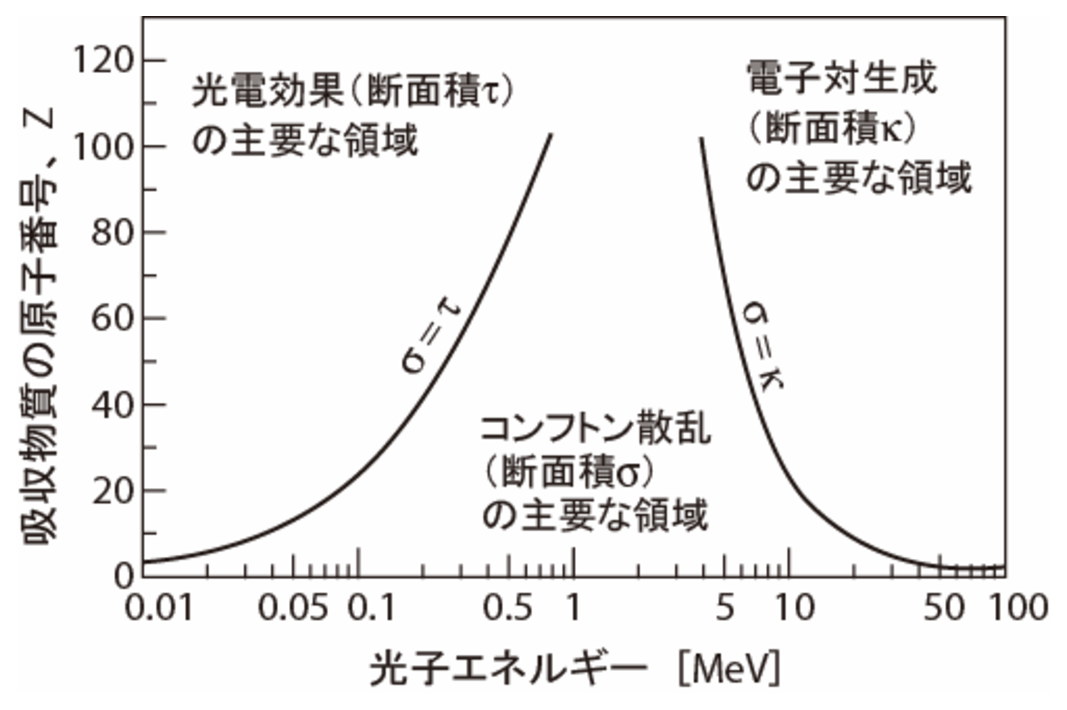
\includegraphics[width=10cm]{image/other/mu_dist.eps}
 \end{center}
 \caption{電磁放射線と物質との相互作用の優勢領域\cite{QA}}
 \label{fig:mu_dist}
\end{figure}











	% 本文2
\chapter{シンチレーション検出器\\(間接変換型検出器)}
\if0
臨床で用いられるCTの光センサーはフォトダイオード(PD)が現在のCTでは最も多く使われている。PDは構造が単純で小型化が容易であり、印加電圧が小さく消費電力が小さいという利点がある。しかし、素子自体が増幅機能を持たないため信号が小さくノイズに弱いことが最大の欠点である。そのため、鮮明なCT画像を取得するためには$10^{8-9}$cts/mm$-2$もの量のX線照射量が必要となっている。つまり「信号がノイズに埋もれない」ことが、現在のCTのX線照射量を決める要因となっていいる。\\
そこで本研究では素子の内部増幅機能に着目し、内部増幅を持つアバランシェフォトダイオード(Avalanche Photodiode: APD)、またはMulti-Pixel Photon Counter (MPPC)を利用することでノイズの影響を極端に抑え、PDを用いた従来型CTよりはるかに低線量で同等以上の画像の取得が可能であると考えた。またその低線量下であればMPPCによるフォトンカウンティングも可能となり、エネルギー情報を利用した多色イメージングも実現できCTの画像診断に新たな可能性を切り拓くことができる。本章では従来の光センサーであるPDと次世代光センサーAPDとMPPCの基本特性について述べる。
\fi
従来のX線CTの検出器にはシンチレータとフォトダイオード(Photodiode : PD)が最もよく用いられる。本章ではまずシンチレータの特徴とPDの構造と性能について述べ、その後内部増幅機能を持つアバランシェフォトダイオード(Avalanche Photodiode : APD)、Multi-Pixel Photon Counter (MPPC)それぞれの構造や性能について述べる。

\section{シンチレータ}
シンチレータとは放射線を吸収して,そのエネルギーによって蛍光する物質の総称である。シンチレータは通常,放射線を吸収したらすぐに蛍光を発し始める($10^{-8}$s 以内)。その時間変化
は以下の簡単な指数関数で近似することができる。
\begin{align}
N=\frac{N_0}{\tau_d}\exp{\left(-\frac{t}{\tau_d}\right)}
\end{align}
ここで,$N$ は時間ごとの発光した光子数で,$N_0$ は発光した光子の総数,$\tau_d$は減衰時定数である。立ち上がり時間は減衰時間よりも短く,上の式では簡略化のために省略してある。また,減衰時定数はシンチレータの種類によって固有のものである。\\
\ \ シンチレータには大きく分けて,有機シンチレータ,無機シンチレータ,プラスチックシンチレータがあるが,本節ではCTに用いられる無機シンチレータの原理と特徴を説明する(\Fref{fig:sinti})。
\begin{figure}[H]
 \begin{center}
 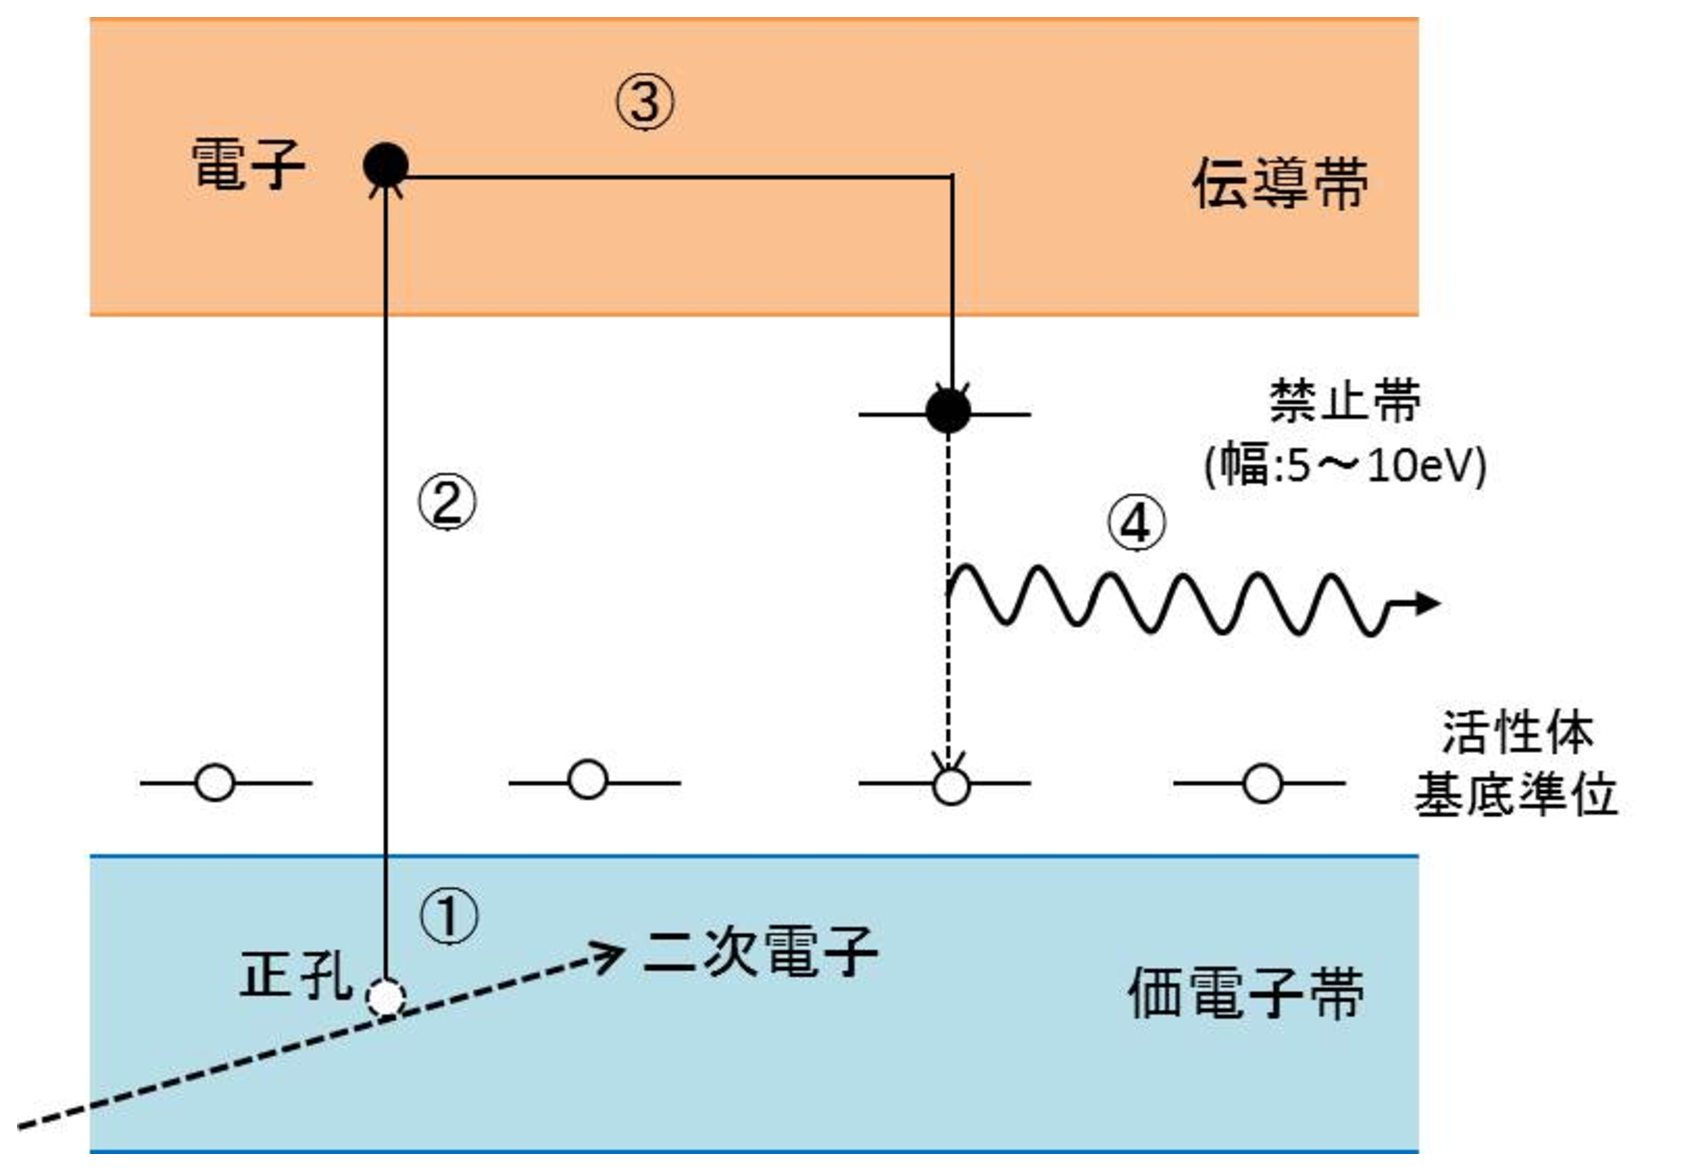
\includegraphics[width=8cm]{image/other/sinci.eps}
 \end{center}
 \caption{シンチレータの発光原理\cite{QA}}
 \label{fig:sinti}
\end{figure}

\begin{enumerate}
\item 入射光子が無機シンチレータ中に入ると前章で述べたような光電吸収,コンプトン散乱,電子対生成などの相互作用を起こし,シンチレータ内に二次電子が発生し,この電子がシンチレータの束縛電子を励起することで価電子帯から伝導帯に遷移し電子-正孔対が生じる。
\item 励起された電子と価電子帯の正孔が緩く結合する(励起子:exciton)
\item 伝導帯を移動中の電子が捕獲され,活性体原子は励起状態となる。
\item 励起準位の活性体原子は寿命(蛍光時定数)に応じて可視光を放出し基底状態に遷移する。
\end{enumerate}

\if0
まず,入射光子が無機シンチレータ中に入ると前章で述べたような光電吸収,コンプトン散乱,電子対生成などの相互作用を起こし,シンチレータ内に自由電子が発生しこの電子がシンチレータの束縛電子を励起することで価電子帯から伝導帯に遷移し電子-正孔対が生じる。このとき,伝導帯には電子が価電子帯の正孔に遷移することが可能となる。しかしながら純粋な結晶の場合,電子が伝導帯から光子を放出して価電子帯に遷移する場合,禁止帯(8eV程度)が大きいため可視光とならない。\\
\ \ そこで,少量の不純物を結晶中に添加し,純粋結晶の禁止帯中に価電子帯への電子の遷移が可能な新しいエネルギー状態を形成する。入射光子との相互作用によって生じた自由電子は,電子を価電子帯から伝導帯へ上げて数多くの電子正孔対を作る。この時,活性化物質の電離エネルギーは通常の光子位置のそれよりも小さいので小さいので正孔は素早く活性化物質の位置へ移動してそれを電離する。一方,伝導帯の電子は電離された活性化物質に移動する。この結果,活性化物質は励起状態になり上がり,基底状態に遷移する際に可視光を放出する。
\fi


入射光子のエネルギーが高いほど多くの励起子が生じ,生じる可視光の光子数が多くなり,強い蛍光となる。すなわち,シンチレータによって入射光子のエネルギーに比例する蛍光をえることができる。\\\ \ また,シンチレータの中には単結晶と多結晶(セラミック)のものがあり,単結晶においては,歩留まりが悪く,大型のものは製作が困難で高額になりやすく,大型化に限界がある。一方,多結晶は大型化が容易であるが,透明度が悪いため,光子が光検出器に届きにくという問題点があるが,近年様々なシンチレータのセラミック化が研究されている。\\\ \ シンチレータに要求される特性および性質として以下のようなものが挙げられる。以下全てを満たすシンチレータは存在しないため、目的に応じて適切なシンチレータを選ぶ必要がある。

\begin{itemize}
\item 放射線エネルギーの蛍光への変換効率(発光量)[ph/MeV]が高い\ (Tl:NaI,Tl:CsI,\\
Ce:GAGG,LaBr$_3$,LaCl$_3$など)\\
\item 放射線の阻止能が高い$\propto\rho Z^4_{eff}$ (BGO,Ce:LYSO,PWOなど) \\
高密度かつ原子番号高いほど,入射放射線と相互作用(特に光電吸収)が起きやすくなり,放射線の阻止能があがりカウントレートが増える。
\item 蛍光の減衰時定数が短い\ (Pr:LuAG,Ce:LYSO,Ce:YAP,Ce:GSOなど)\\
時定数短いとパイルアップしないため,時間分解能が高くなり高計数に対応する。言い方を変えれば高速動作が可能となる。
\item 蛍光の波長分布が,光検出器の分光感度特性に適合している。\\
蛍光の波長分布と光検出器の分光感度特性が適合していると,光子が効率よく光電子に変換されるので,高い量子効率が得られる。
\item 潮解性と自発光(内在バックグラウンド)がない\\\
潮解性がある場合,空気中に置いておくと溶けるので取扱いや保管に注意しなければならない。また,Pr:LuAG
やCe:LYSOは,$^{176}$Luが$\beta$崩壊するときに放出する線を自身で検出してしまい,それがバックグラウンドノイズとなってしまう。
\end{itemize}

\Tref{sinti}に代表的な無機シンチレータの諸性質を示す。
\begin{table}[H]
\begin{center}
\scalebox{0.8}[0.8]{
\begin{tabular}{ccccccc} \hline
シンチレータ & 発光量[ph/MeV] & 最大発光波長[nm] & 減衰時間[ns] & 密度[g/cm$^3$] & 潮解性 & ref \\\hline
Tl:NaI & 41,000 & 410 & 230 & 3.67 & 有 & \cite{sinci} \\
Tl:CsI & 66,000 & 565,420 & 800$\sim$6000 & 4.51 & わすかに有 & \cite{sinci} \\
BGO & 9,000 & 480 & 300 & 7.13 & 無 & \cite{sinci} \\
LaBr$_3$ & 63,000 & 380 & 20 & 5.29 & 有 & \cite{sinci} \\
Ce:GSO & 8,000 & 440 & 60,600 & 6.71 & 無 & \cite{sinci} \\
Ce:YSO & 10,000 & 420 & 37,82 & 4.45 & 無 & \cite{sinci} \\
Ce:LYSO & 30,000 & 420 & 40 & 7.10 & 無 & \cite{sinci} \\
Ce:YAP & 10,000 & 370 & 25 & 5.50 & 無 & \cite{sinci}\\
Ce: Pr:$\rm Gd_2O_2S$(GOS) & 50,000 & 512  & 3,000 & 7.28 &  無 & \cite{hitachi} \\
Ce:GAGG & 46,000 & 520 & 88,258 & 6.63 & 無 & \cite{sinci} \\\hline
\end{tabular}
}
\end{center}
\caption{無機シンチレータとの特性比較}
\label{sinti}
\end{table}


\if0 

\begin{table}[H]
\begin{center}
\begin{tabular}{cccccc} \hline
シンチレータ & 発光量[ph/MeV] & 最大発光波長[nm] & 減衰時間[ns] & 密度[g/cm$^3$] & 潮解性 \\\hline
Tl:NaI & 41,000 & 410 & 230 & 3.67 & 有 \\
Tl:CsI & 66,000 & 565,420 & 800\UTF{FF5E}6000 & 4.51 & わすかに有 \\
Na:CsI & 40,000 & 420 & 630 & 4.51 & 有 \\
BGO & 9,000 & 480 & 300 & 7.13 & 無 \\
CWO & 2,800 & 500 & 3, 17 & 7.90 & 無 \\
PWO & 410 & 440\UTF{FF5E}500 & 5\UTF{FF5E}15 & 8.28 & 無 \\
LaBr$_3$ & 63,000 & 380 & 20 & 5.29 & 有 \\
LaCl$_3$ & 46,000 & 350 & 25 & 3.79 & 有 \\
Ce:GSO & 8,000 & 440 & 60,600 & 6.71 & 無 \\
Ce:LYSO & 30,000 & 420 & 40 & 7.10 & 無 \\
Ce:YSO & 10,000 & 420 & 37, 82 & 4.45 & 無 \\
Ce:YAG & 8,000 & 550 & 70 & 4.57 & 無 \\
Ce:YAP & 10,000 & 370 & 25 & 5.5 & 無 \\
Ce:LSO & 27,300 & 420 & 35\UTF{FF5E}47 & 7.40 & 無 \\
Ce:GAGG & 46,000 & 520 & 88, 258 & 6.63 & 無 \\
Pr:LuAG & 20,000 & 310 & 20 & 6.73 & 無 \\\hline
\end{tabular}
\end{center}
\caption{代表的な無機シンチレータの諸特性}
\label{sinti}
\end{table}
\fi




\section{フォトダイオード(PD)\label{sec:photo}}



\begin{figure}[H]
 \begin{center}
 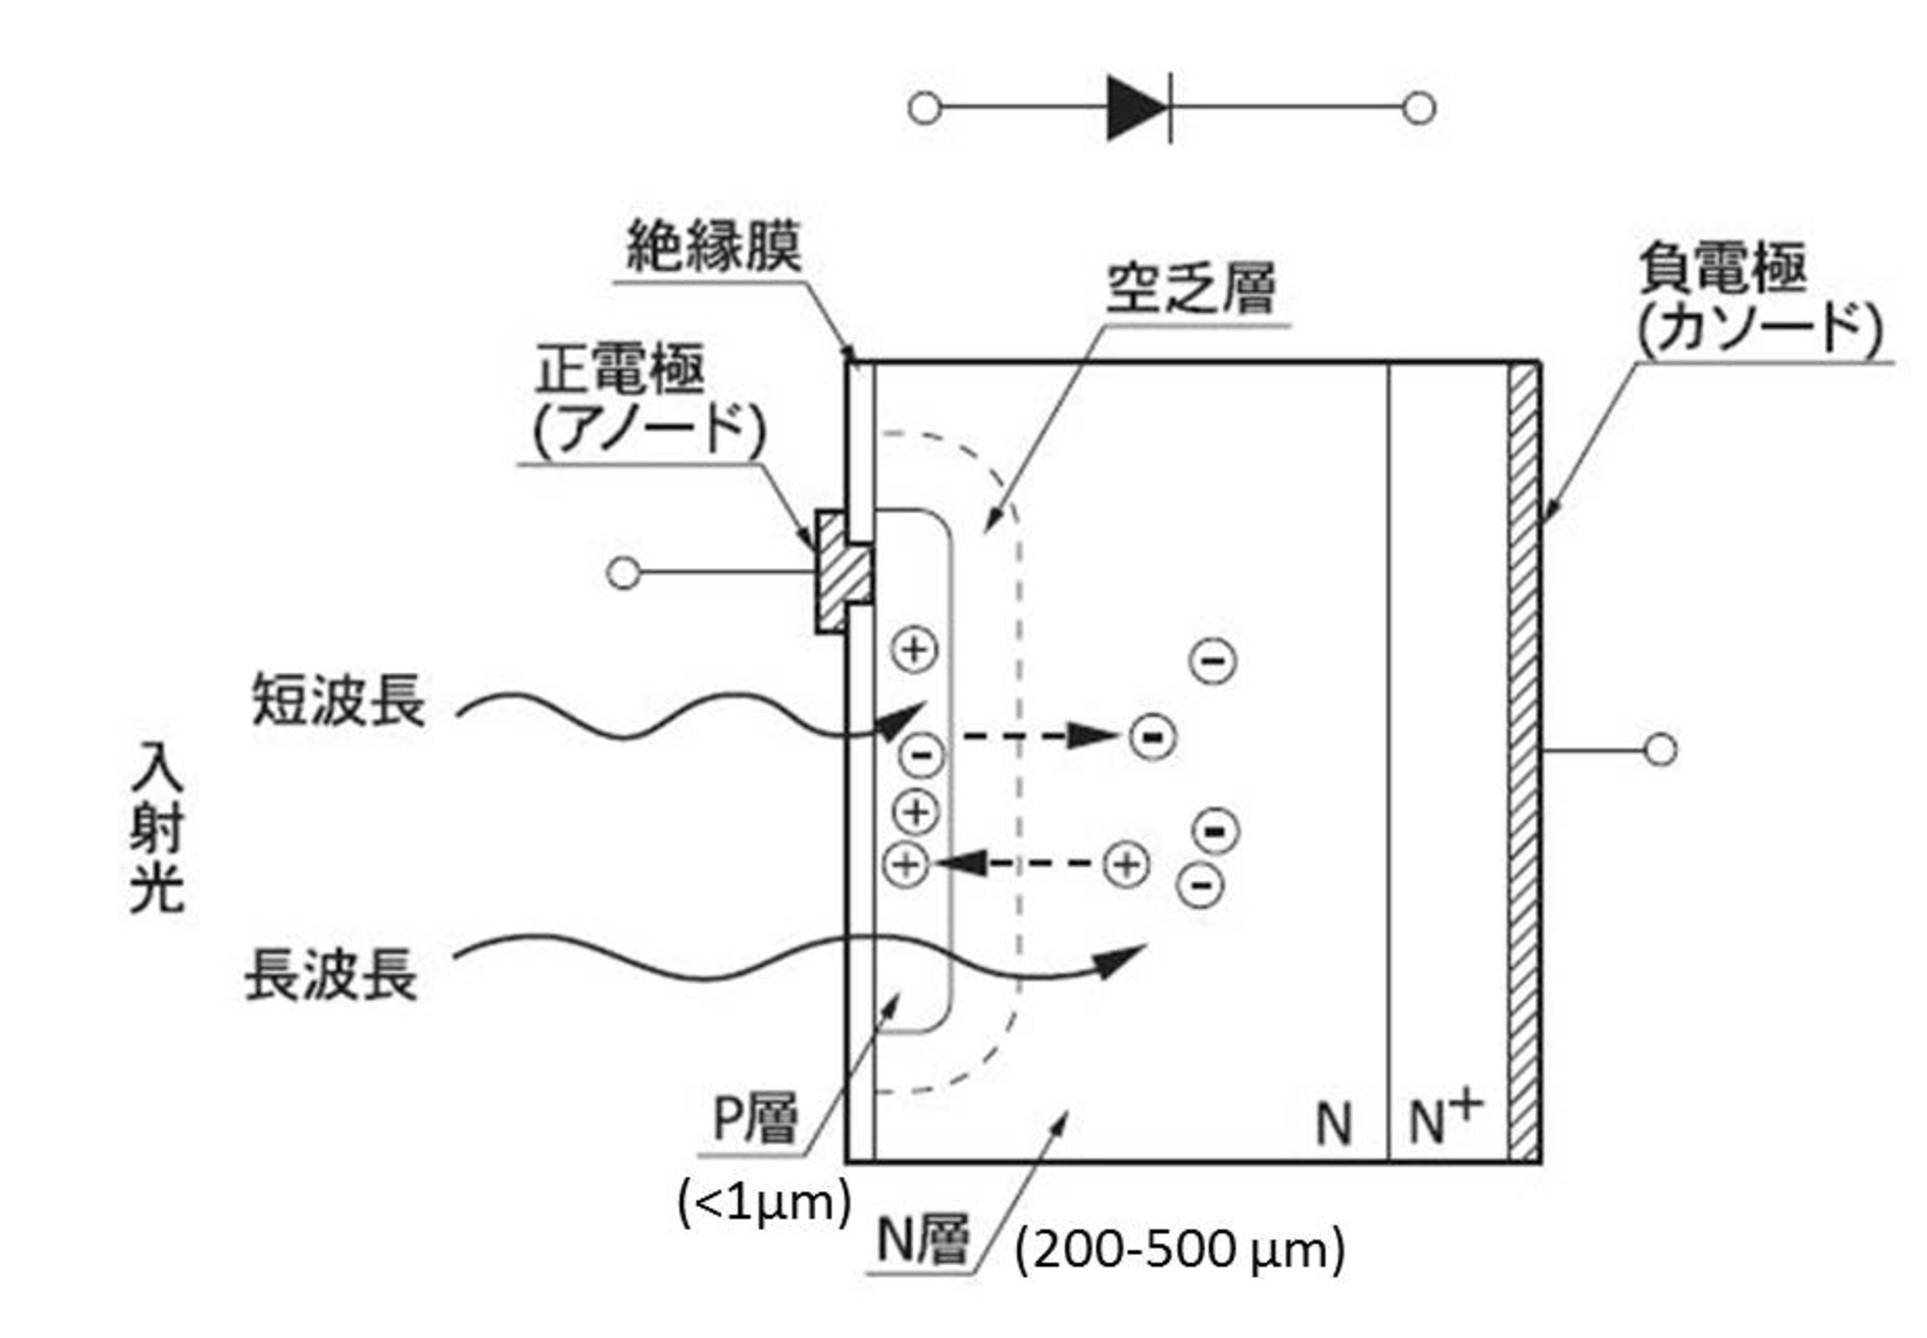
\includegraphics[width=10cm]{image/other/PIN.eps}
 \end{center}
 \caption{Siフォトダイオードの断面構造\cite{hama_hand_2}}
 \label{fig:PIN}
\end{figure}

フォトダイオード(PD)は現在のCTでは最も多く使われている光検出器である。よく用いられているPINフォトダイオードの構造を\Fref{fig:PIN}に示す。光はp型層の入射窓より入る,シリコン本体に入る光の透過をよくするため,この窓はできるだけ薄く作られている。光によって生成された電子と正孔は,逆バイアス電圧(n側が高電圧)で形成されている電界によりそれぞれの電極に収集される。ここで誘起される電荷は接続されている前置増幅器に送られ,出力パルスを発生する。\\
典型的なシンチレーション事象では可視光光子は数千個\footnote{CTにおいてはGOS(40,000ph/MeV)が用いられるが60keVがシンチレータで光電吸収されたとし、PDの量子効率を50\%とすれば生成する可視光の数は$N =60\times 40\times 0.5=1200$ 個
となる}しか生成されないのえ、得られる電荷パルスは非常に小さく、内部増幅機能も持たないためパルスモード動作ではノイズが最大の問題となる。そこで,パルスモードではなく電流モードでは頻繁に発生する多くのシンチレーション事象を蓄積することにより固有のノイズに打ち克つことが可能となり,結果的に優秀な特性を得ることができる。さらにフォトダイオードは構造が単純で小型化が容易かつ印加電圧が数十$\sim$数百Vで十分なので消費電力が少ないことから、シンチレータと組み合わせ電流モードで読み出すことで、X線CTの光検出器として選択されるようになってきた。\\
フォトダイオードの電子ノイズとして次の三つのものが最も重要である。
\begin{enumerate}
\item 並列ノイズの成分であるバルク中に生成される漏れ電流のゆらぎ
\item もう一つの並ノイズの成分である表面の漏れ電流のゆらぎ
\item 直列ノイズ源である直列抵抗に伴うノイズあるいは検出器の電気接触不良
\end{enumerate}
また、暗電流の温度依存性を\Fref{fig:PD_darkcurrents}に示す。



\if0
\begin{figure}[H]
 \begin{center}
 \includegraphics[bb=,width=1\hsize]{image2/chapter5/.png} 
 \end{center}
 \caption{フォトダイオードの暗電流の温度依存性}
 \label{fig:PD_darkcurrents}
\end{figure}
\fi


\begin{figure}[H]
 \begin{center}
 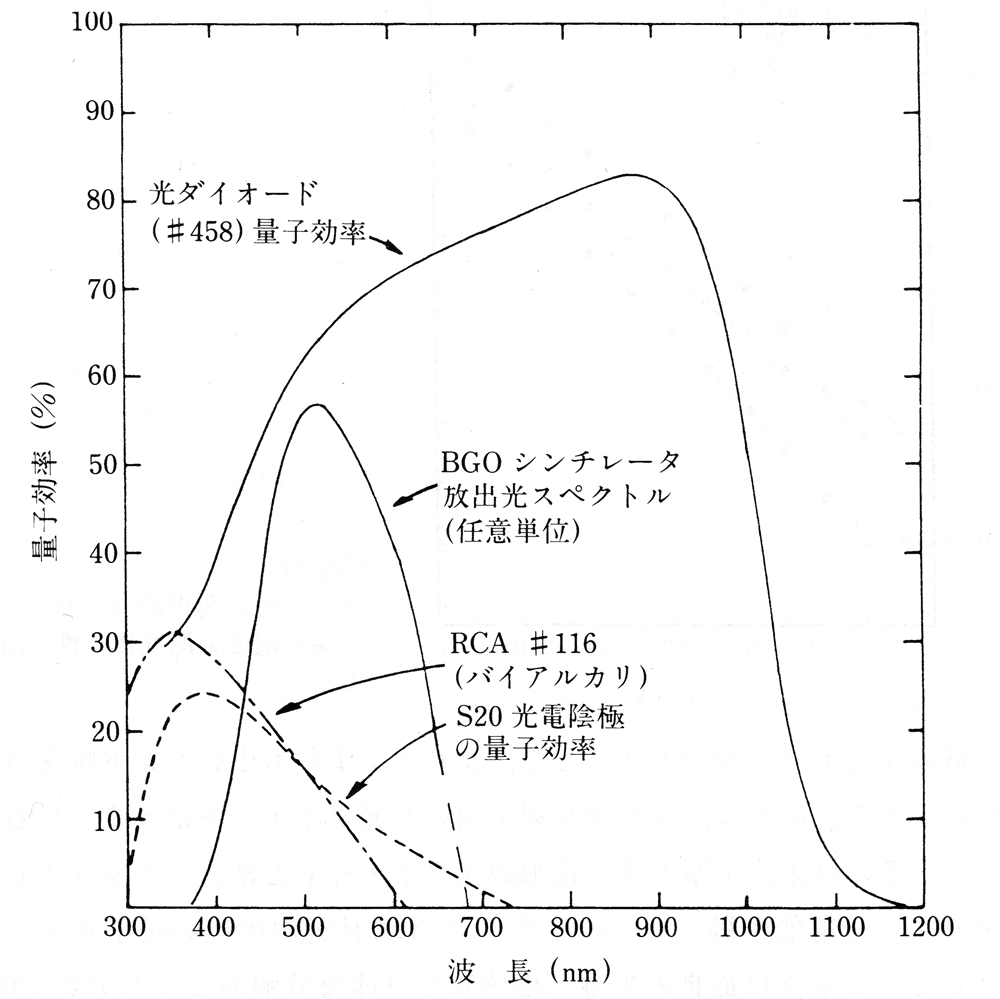
\includegraphics[width=10cm]{image/other/PD_PDE.eps}
 \end{center}
 \caption{Siフォトダイオード(#458)と代表的なバイアルカリとS-20光電面の量子効率の比較とBGOシンチレータの発光波長分布\cite{radiation_handbook}}
 \label{fig:ryousi_PD}
\end{figure}


以下にフォトダイオードのシンチレーション計数(間接型検出)における,利点・欠点についてまとめる。
\begin{itemize}
\item 利点

\begin{itemize}
\item 構造が単純で小型化が容易
\item PMTの印加電圧1000Vに対し,フォトダイオードは数十$\sim$数百Vの印加電圧で十分なので消費電力が少ない
\item 量子効率が高い(60$\sim$80$\%$)のでエネルギー分解能が高い
\item 高い量子効率が広い波長領域におよぶ
\item 磁場の影響を受けないので,磁場が存在するため光電子増倍管が使えない実験に代わりに用いることができる。
\item 電流モード読み出しにおいては安定する。
\end{itemize}

\item 欠点
\begin{itemize}
\item 増幅機能を持たないため信号が小さく,パルスモード読み出しにおいてノイズが問題となる。特に低エネルギー放射線の検出には不向きである。
\item 応答速度はシンチレータの時定数に依存する。
\item SiやGeダイオードではバンドギャップが小さいため室温おける暗電流のためノイズが多い。
\end{itemize}

\end{itemize}




\section{Avalanche Photodiode(APD)\label{sec:APD}}
PMTは高い増幅率を持つが,量子効率が低い。PDは量子効率が高いが増幅機能を持たない。PMTとPDの両方の長所を兼ね備えた光センサーがAPDである。APD においては半導体内部に高い勾配電場を作ることで,光や放射線によって電子・正孔対ができると,それが強い電場領域に入るとことで加速され,衝突電離を起こす。この衝突電離によって発生した電荷や正孔がまた同様に衝突電離を起こす,といったことを繰り返して,なだれ増幅(avalanche)を起こす。この結果,電子や正孔はM=50$\sim$100 倍まで増幅されて電極から読み出される。つまり,ノイズを等価的に1/Mに低減することで通常のPDより遥かに優れたS/N比を得ることができる。\\
\ \ APDには従来の斜めエッジ型,リバース型,リーチスルー型があるが,シンチレーション検出器としてはリバース型(\Fref{fig:reverce})が適切である。

\begin{figure}[H]
 \begin{center}
 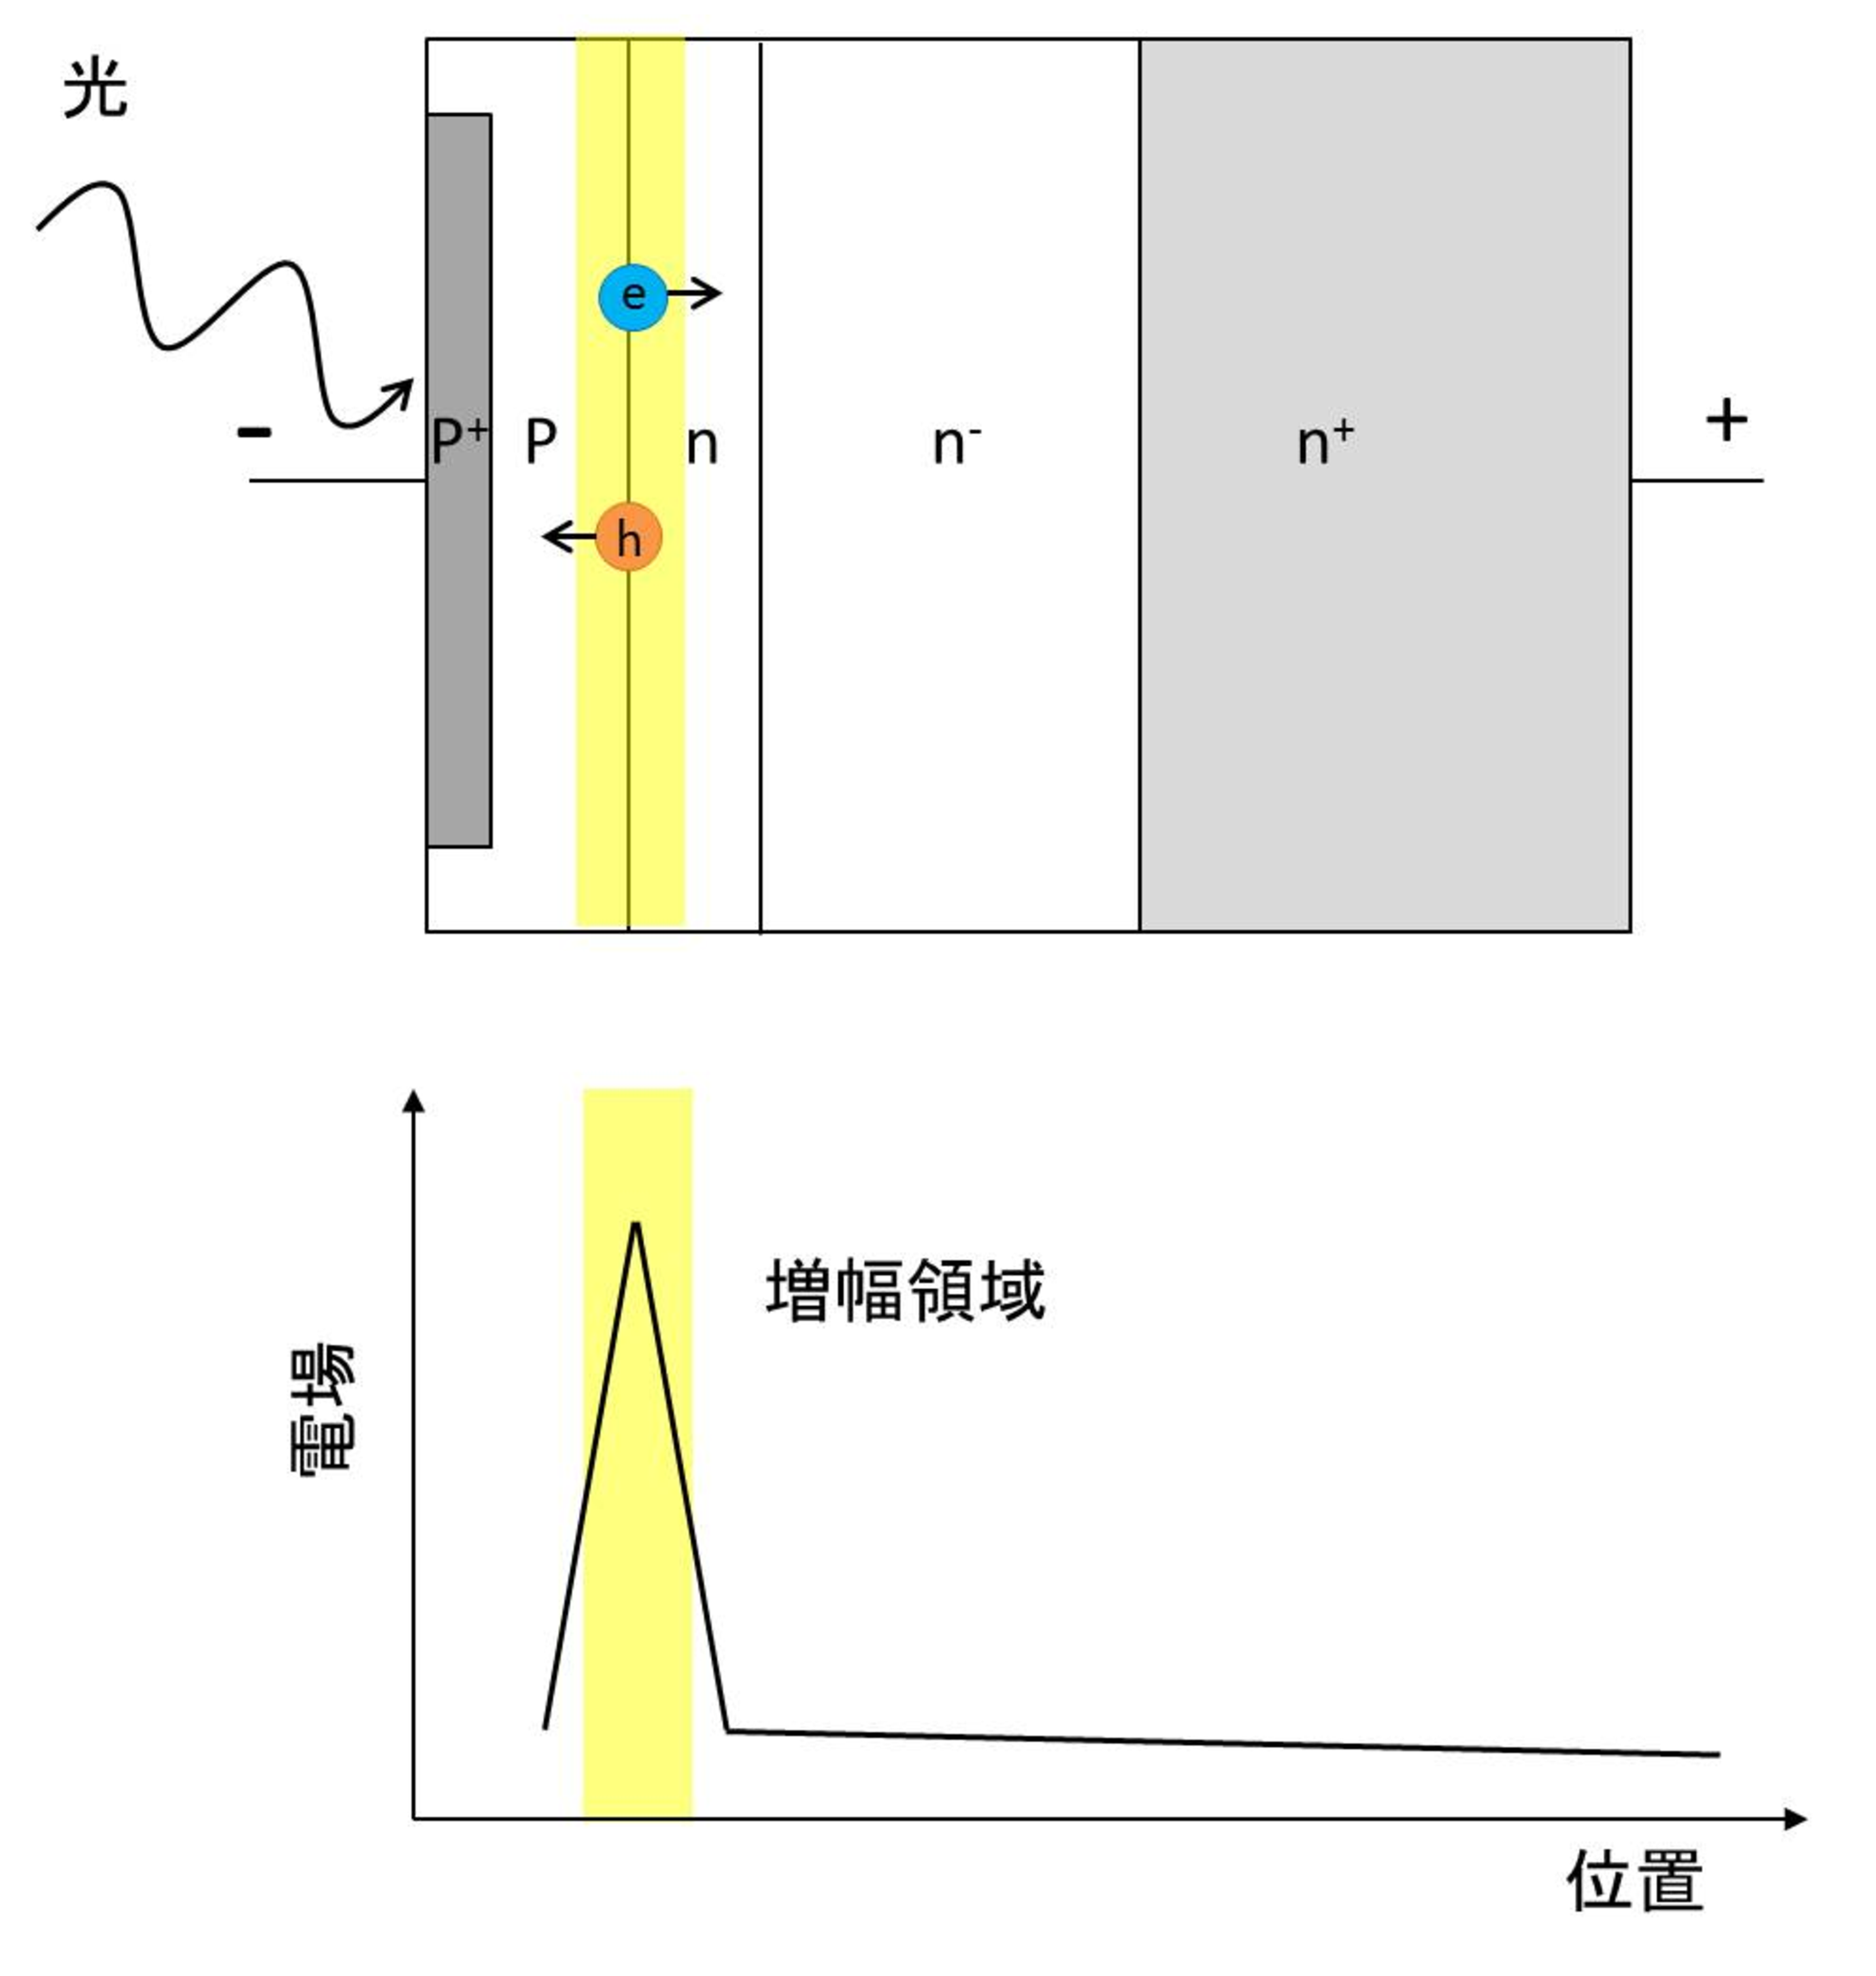
\includegraphics[width=10cm]{image/other/reverce.eps}
 \end{center}
 \caption{リバース型APDの構造\cite{kataoka_web}}
 \label{fig:reverce}
\end{figure}

この構造は入射面から$5\mu$m程度のところに増幅領域があり,シンチレーション光が表面で吸収され電子正孔対に変換されると,その全てを増幅することができる。このとき信号は増幅されるが熱電子は増幅されないので暗電流を小さくすることができノイズだけを約1/100まで低減できるのが最大の利点である。また空乏層は薄い(40$\mu$m程度)ので300-400V程度の低電圧で十分な増幅率を得ることができる。以下にAPD(リバース型)のシンチレーション検出器としての利点と欠点をまとめる。
\begin{itemize}
\item 利点
\begin{itemize}
\item PMTとPDの両者の利点(高い量子効率($\sim80\%$)\ +\ 高い増幅率(100倍))を持つので高いエネルギー分解能,高いS/N比を得る
\item 高い増幅率を得たことにより低エネルギーの放射線についてもパルスモードでの読み出しが可能となりエネルギー分解能が通常のPDより改善
\item コンパクト,低電圧動作(300-400V),磁場に強い
\item 暗電流が小さい
\end{itemize}

\item 欠点
\begin{itemize}
\item 増幅率はPMTの増幅率($10^{5-6}$)程及ばない
\end{itemize}

\end{itemize}


%一方,電流モードについては,通常のPDは増幅機能はないが固有の安定性があるのでAPDよりも好んで使われる。

\section{Muliti-Pixel Photon Counter(MPPC)\label{sec:MPPC}}
MPPCとは,Si-PM(Silicon\ Photomultiplier)と呼ばれるデバイスの一種で,個別に動作する複数のガイガーモードAPDを数十ミクロンのピッチでピクセル状に並べたデバイスである。APDの逆電圧を降伏電圧以上にするとパルス出力の大きさは入射フォトン数に関係なく素子固有の飽和出力が発生し(ガイガー放電),光子が入射したか入射しないかという情報だけが分かることになる。この電圧でAPDを動作させる状態をガイガーモードという。ガイガーモードAPDのゲインは$10^5-10^6$でありこの高い増幅率により1光子レベルの微弱な信号にも高いS/N比を実現し,微弱な光でも検出することができる。MPPCに用いられるAPDの基になっているのは\ref{sec:APD}で述べたリバース型のAPDである。MPPCの等価回路と1つのAPDピクセルと動作原理を\Fref{fig:geiger}に示す。
 \begin{figure}[H]
 \hspace{1cm}
 \begin{minipage}{0.4\hsize}
 \begin{center}
 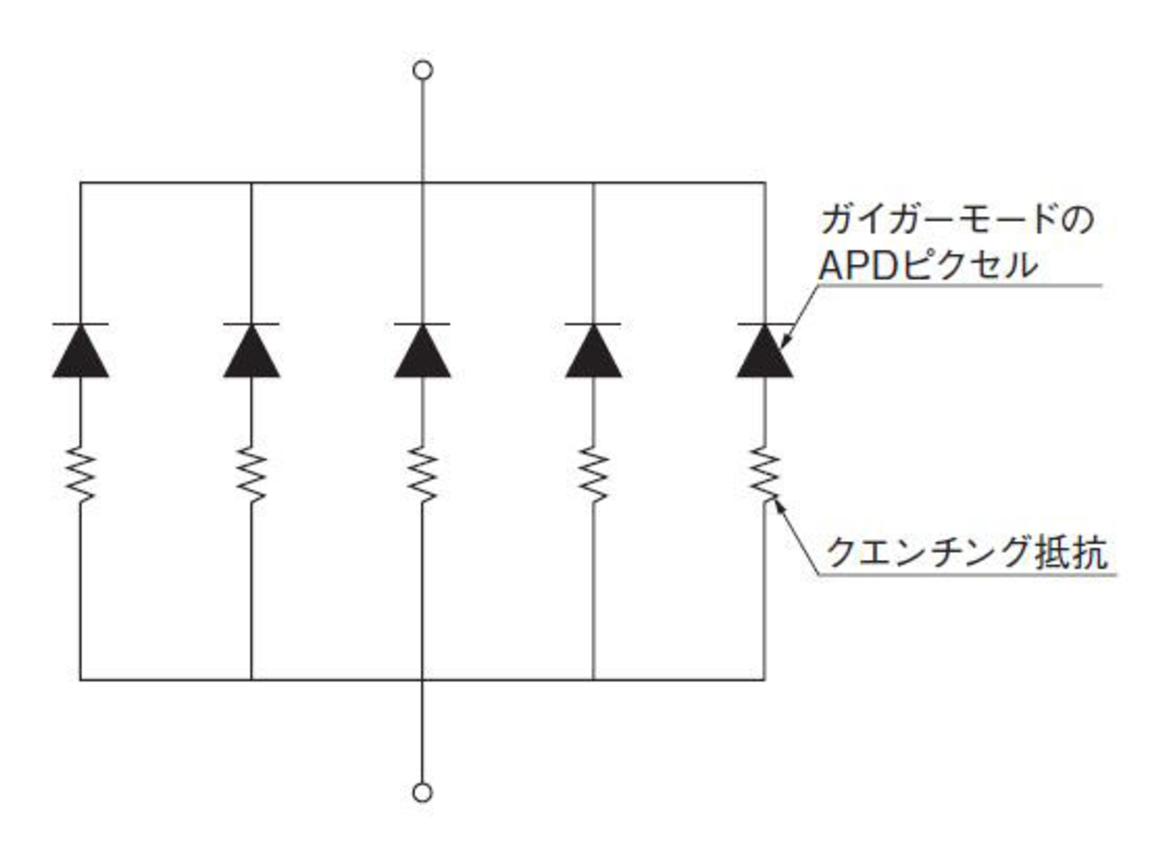
\includegraphics[width=8cm]{image/other/MPPC_touka.eps}
 \end{center}
 \end{minipage}
 \hspace{2cm}
 \begin{minipage}{0.2\hsize}
  \begin{center}
 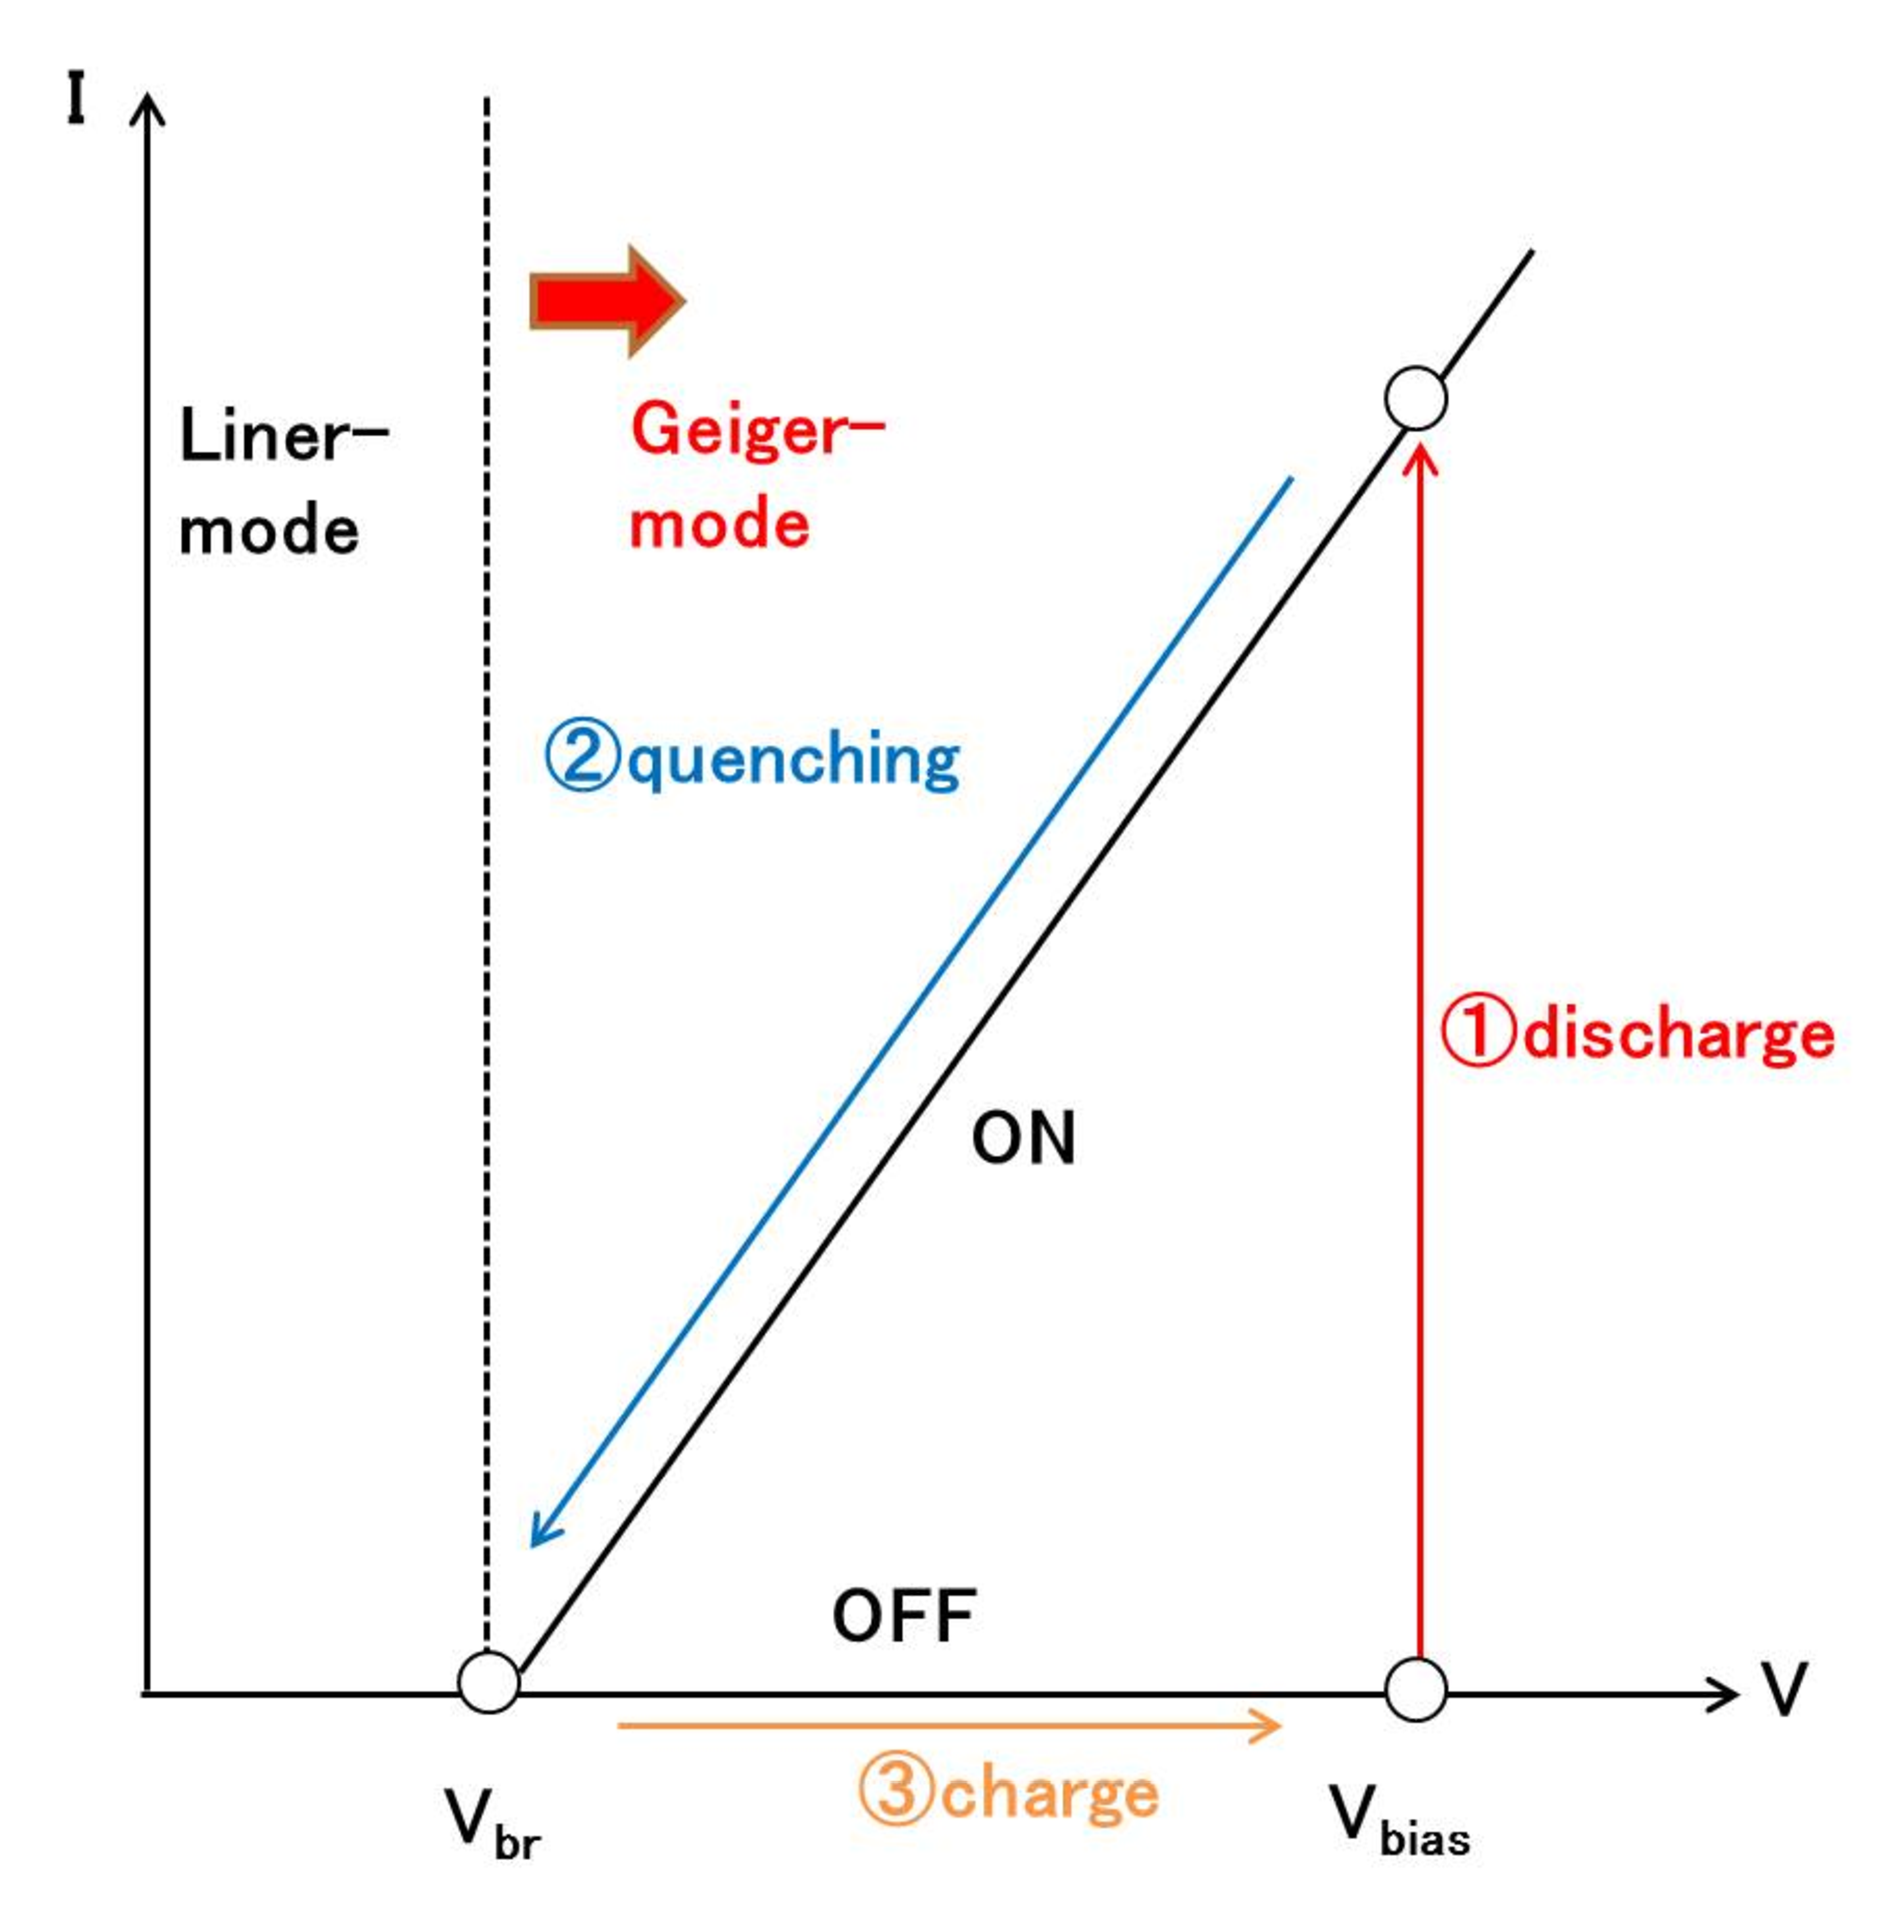
\includegraphics[width=6cm]{image/other/MPPC_cicle.eps}
 \end{center}
 \end{minipage}
 \caption{MPPCの等価回路(左)\cite{hama_MPPC}とMPPCのガイガー放電サイクル(右)}
 \label{fig:geiger}
\end{figure}

動作原理は以下の3つのサイクルの繰り返しである
\begin{enumerate}
\item 光子が入射しガイガー放電が生じる(discharge)
\item ガイガー放電された電流がクエンチング抵抗に流れると電圧降下が起こりAPDにかかる電圧が降伏電圧以下になるとガイガー放電が止む(quenching)
\item ガイガー放電が止むと電圧降下は起こらなくなり再びAPDにかかる電圧が降伏電圧以上になりガイガー放電が起きる状態となる(charge)
\end{enumerate}
この1サイクルには50ns$\sim$100nsかかりこの時間に光子が入射しても光子が検出できず不感時間となってしまう。ガイガー放電による1ピクセルからの出力電荷はAPDピクセルの容量を$C$,バイアス電圧を$V_{\rm op}$,降伏電圧を$V_{\rm br}$として以下のように書ける。
\begin{align}
Q_{\rm out}=C(V_{\rm bias}-V_{\rm br})\label{eq:out}
\end{align}
つまり,出力電荷はAPDピクセルの容量とバイアス電圧に比例する。複数のフォトンが複数のピクセルに入射するとそれぞれのピクセル出力の和がMPPCの出力となり,励起したAPDピクセルの数$N_{\rm fired}$を\Eref{eq:out}にかけた$Q_{\rm out}\times N_{\rm fired}$が全出力となる。またゲイン$M$は$M\equiv Q_{\rm out}/e$と定義されゲインもバイアス電圧とAPDの容量に比例する。APDピクセルサイズが大きい程APD容量は大きくなりゲインは上がる。またピクセルサイズが大きほどピクセルに対する受光部の割合が増え開口率があがるので検出効率が高くなる。ただしピクセルサイズが大きいほどダイナミックレンジ(同時に検出できるフォトン数)が下がる。逆にAPDピクセルサイズが小さいほど,容量は小さくないり,ゲイン,開口率,検出効率は下がるが,ダイナミックレンジは上がる。以下にMPPCの利点と欠点を示す。


\begin{itemize}
\item 利点

\begin{itemize}
\item 低電圧(100V以下)で動作可能
\item ガイガーモードで動作させることでAPDによりも高くPMTに匹敵する高いゲイン($10^5-10^6$)を持ちノイズに強い
\item 速い時間応答($\sim$100ps)
\item 小型であり磁場の影響を受けない
\item 常温でも動作可能
\end{itemize}

\item 欠点
\begin{itemize}
\item 検出効率(PDE:Photon\ Detection\ Efficiency)が高くない\\ APDよりゲインがはるかに高くなったが,クエンチング抵抗のスペース,ピクセル間がデッドスペースとなりAPDやPDほど検出効率(検出したフォトンのうち何$\%$を検出できるか)が高くない($\leq60\%$)
\item ゲインに温度依存性がある\\常温での動作が可能だがゲインに温度依存性があり,一定のバイアス電圧に対するゲインは温度が低いほど高く,温度が高いほど低くなる\footnote{温度が上がると結晶の格子振動が激しくなり,加速されたキャリアのエネルギーが十分に大きくならないうちに結晶と衝突する確率が高くなり,イオン化が起こりにくくなる。その結果温度が高いほどゲインが低くなる。}。そのため一定の出力を得るには温度によってバイアス電圧を変化させるか,素子の温度を一定に保つ必要がある。
\item 入射フォトン数が多くなると励起ピクセル数と入射フォトン数の線形性が崩れる\\MPPCの全ピクセル数$ N_{\rm total}$がダイナミックレンジを決定し,全ピクセル数に対して入射フォトン数$ N_{\rm photon}$が多くなると,1ピクセルに2個以上の光子が入り始め,入射フォトン数と励起ピクセル数$ N_{\rm fired}$の線形性が崩れる\footnote{$ N_{\rm fired}= N_{\rm total}\left[1-\exp{\left(-\frac{ N_{\rm photon}\times \rm PDE}{ N_{\rm total}}\right)}\right]$}。
\item ダークカウントが生じる\\光により生成したキャリアだけでなく熱的に発生したキャリアによっても電流が発生する(ダークカウント)。これは温度が低いほど小さくなる。
\item アフターパルスが生じる\\ 発生したキャリアが結晶欠陥にトラップされ,それが遅れて解放されたときに信号以外のパルスを発生させてしまう(アフターパルス)。温度が低いほどキャリアが欠陥にトラップされる確率が高くなり,アフターパルスは増加する。
\item クロストークが生じる\\
ガイガー放電中に電子と正孔が再結合して光子が放出され,その光子をとなりのピクセルが検出してガイガー放電を起こしてしまうことがある(クロストーク)

\end{itemize}

\end{itemize}

\section{光検出器の性能比較}

\begin{table}[H]
\begin{center}
\begin{tabular}{ccccc} \hline
 & PMT & PD & APD & MPPC \\\hline
増幅率(ゲイン) & $10^{5-6}$ & 1 & 10-100 & $10^{5-6}$ \\
量子効率(検出効率) & $\leq25\%$ & \multicolumn{2}{c}{$\leq80\%$} & $\leq60\%$ \\
体積・サイズ& ×(大きい) & \multicolumn{3}{c}{$\circ$(小さい)} \\
磁場耐性 & ×(不可) & \multicolumn{3}{c}{$\circ$(可能)} \\
構造 & ×(複雑) & \multicolumn{3}{c}{$\circ$(単純)} \\
動作電圧[V] & $\thicksim1000$ & $\thicksim30$ & $\thicksim300$& $\thicksim70$ \\
電力&×(大)&\multicolumn{3}{c}{$\circ$(小)}\\\hline
\end{tabular}
\end{center}
\caption{光検出器の性能比較\cite{kataoka}}
\label{detectors}
\end{table}
それぞれの光検出器の性能比較を\Tref{detectors}に示す。どれも一長一短であり,用途により選択が必要となる。高いエネルギー分解能を求める場合,量子効率が高いPDやAPDを用いるべきであるが,この二つはゲインが低いので微弱な光つまり,低エネルギーの検出は苦手とする。微弱な光の検出をする場合高いゲインを持つPMTやMPPCを用いるべきである。\\
\ \ CTの光検出器としは小型化が可能なPDが主流である。PDを電流モードで読み出すことによりノイズに打ち勝ち低エネルギーの検出も可能としてる。しかし,フォトンカウンティングCTにおける検出器のためにはパルス読み出しを行う必要があるため高いS/N比を得ることができ,エネルギー分解能も高く,小型化が可能な検出器が求められる。

\chapter{半導体検出器(直接変換型検出)}
\section{CdTe半導体の特性}
従来,X 線やガンマ線の検出のための半導体検出器として,主にシリコン(Si)やゲルマニウム(Ge)が使用されてきた。しかし,Siは原子番号が14と低いためX線やガンマ線に対する検出効率が低く,直接型の半導体検出器としては用いることができない。Geは原子番号が32であり,検出効率は低くはなく,直接型の半導体検出器として用いることで極めて高いエネルギー分解能を得ることできる。しかしGeは室温ではバンドギャップが小さく比抵抗極めて小さいため,液体窒素温度で動作させる必要がある。そこでSi,Geよりも原子番号が高く,検出効率の高いかつ室温動作が可能な化合物半導体としてCdTe(テルル化カドミウム)やCd$_{1-x}$Zn$_x$Te(CZT)がある。それぞれの半導体の特性を\Fref{semi_chara}に示す。
\begin{table}[H]
\begin{center}
\begin{tabular}{ccccc} \hline
半導体(温度[K]) & Si(300) & Ge(77) & CdTe(300) & $\rm Cd_{0.8}Zn_{0.2}Te$(300) \\\hline
原子番号 & 14 & 32 & 48/52 & 48/30/52 \\
密度[g/cm$^3$] & 2.33 & 5.32 & 5.85 & 6.0 \\
バンドギャップ[eV] & 1.12 & 0.74 & 1.5 & 1.6 \\
電離エネルギー[eV] & 3.61 & 2.98 & 4.43 & 5.0 \\
比抵抗[$\Omega\cdot$cm] & $10^3$ & $10^2$ & $10^9$ & 3$\times10^{10}$\cite{takahashi} \\
移動度$\mu_e$[cm$^2$/Vs] & 1350 & 3.6$\times10^4$ & 1100 & 1350 \\
移動度$\mu_h$[cm$^2$/Vs] & 480 & 4.2$\times10^4$ & 100 & 120 \\
寿命$\mu_e$[s] & 2$\times10^{-5}$ & 2$\times10^{-5}$ & 3$\times10^{-6}$ & $\times10^{-6}$ \\
寿命$\mu_h$[s] & 2$\times10^{-5}$ & 2$\times10^{-5}$ & 2$\times10^{-6}$ & 2$\times10^{-7}$ \\
$\mu_e\tau_e\rm[cm^2/V]$ & 0.42 & 0.72 & 3.3$\times10^{-3}$ & $\sim10^{-3}$ \\
$\mu_h\tau_h\rm[cm^2/V]$ & 0.22 & 0.84 & 2$\times10^{-4}$ & $\sim2\times10^{-5}$ \\
参考文献 & \cite{sakai} & \cite{sakai} & \cite{Bellazzini} & \cite{McGregor} \\\hline
\end{tabular}
\end{center}
\caption{半導体の諸特性}
\label{semi_chara}
\end{table}

CdTeのバンドギャップは1.5eVであり,室温動作が可能である。さらにCdTeはSiやGeよりもはるかに高い原子番号を持っているのでSiやGeよりもX線,ガンマ線に対する検出効率が高く,より大きな光電吸収断面積をもっている。\Fref{fig:efficiency}に60keVと120keVのガンマ線に対する検出効率のSi,Ge,CdTeの比較を示す。また\Fref{fig:liner_comp}Si,Ge,CdTeにおける光電効果,コンプトン散乱,電子対生成における線源弱係数の比較を示す。

\begin{figure}[H]
\begin{minipage}{0.5\hsize}
 \begin{center}
 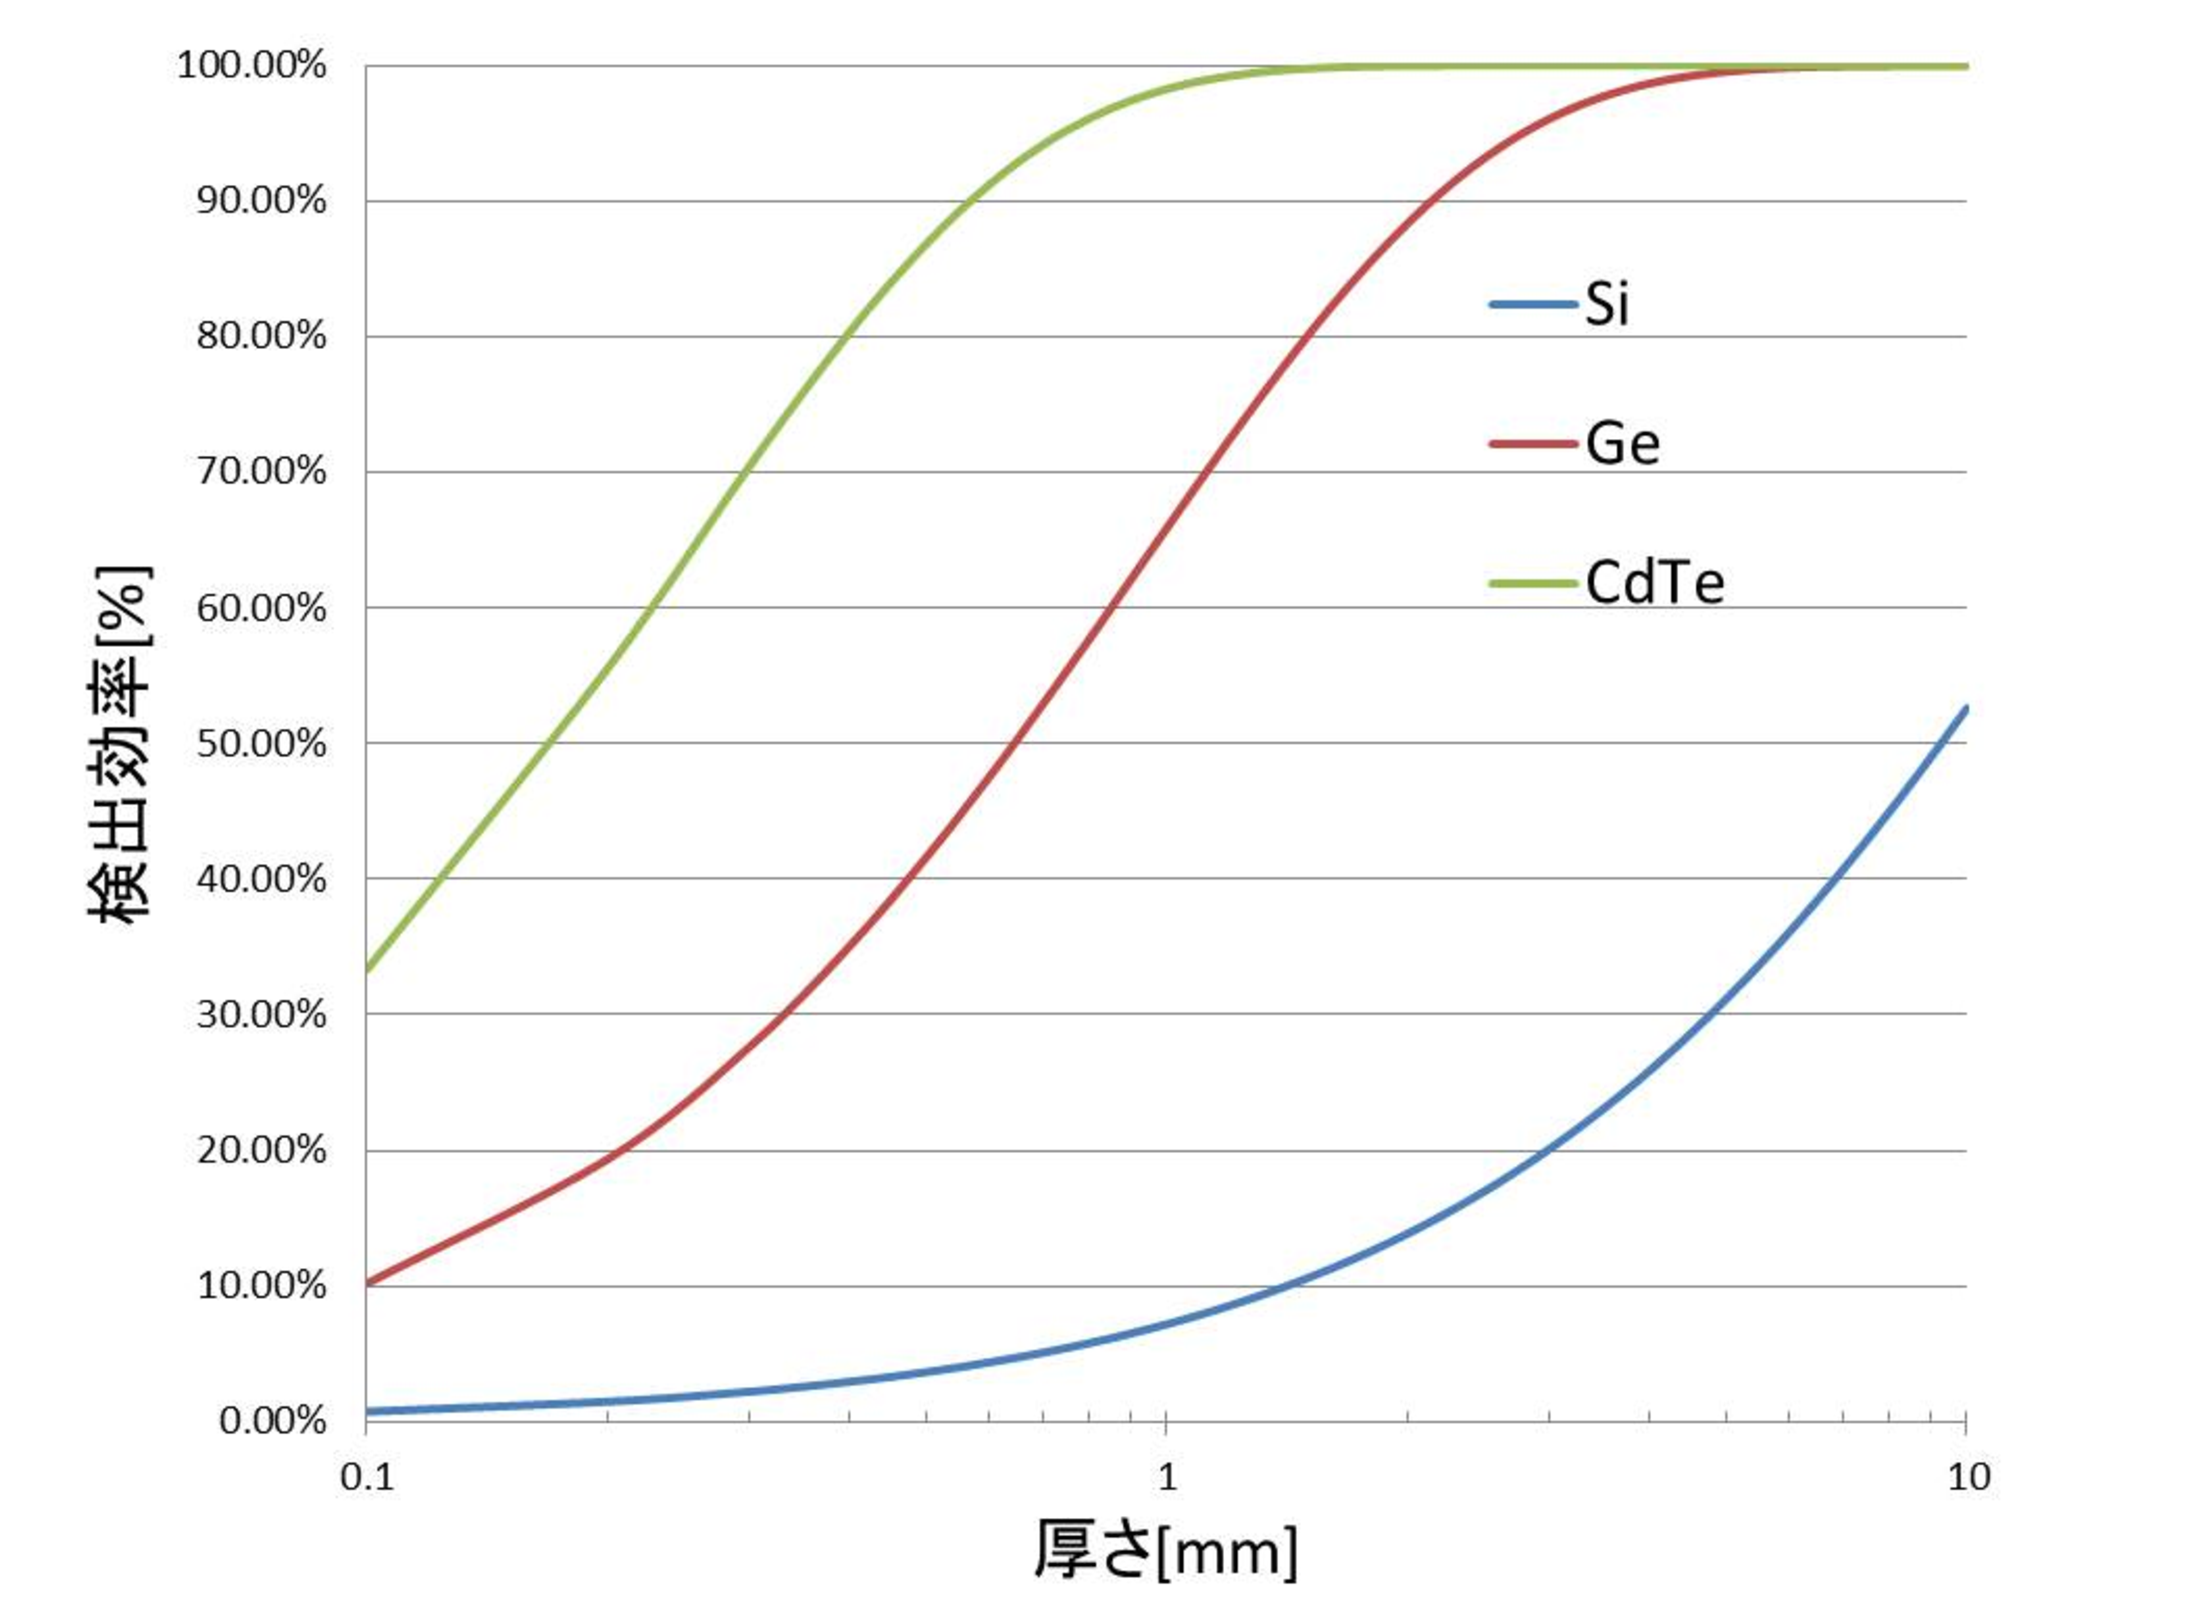
\includegraphics[width=8cm]{image/other/PDE_60.eps}
 \end{center}
 \end{minipage}
 \begin{minipage}{0.5\hsize}
 \begin{center}
 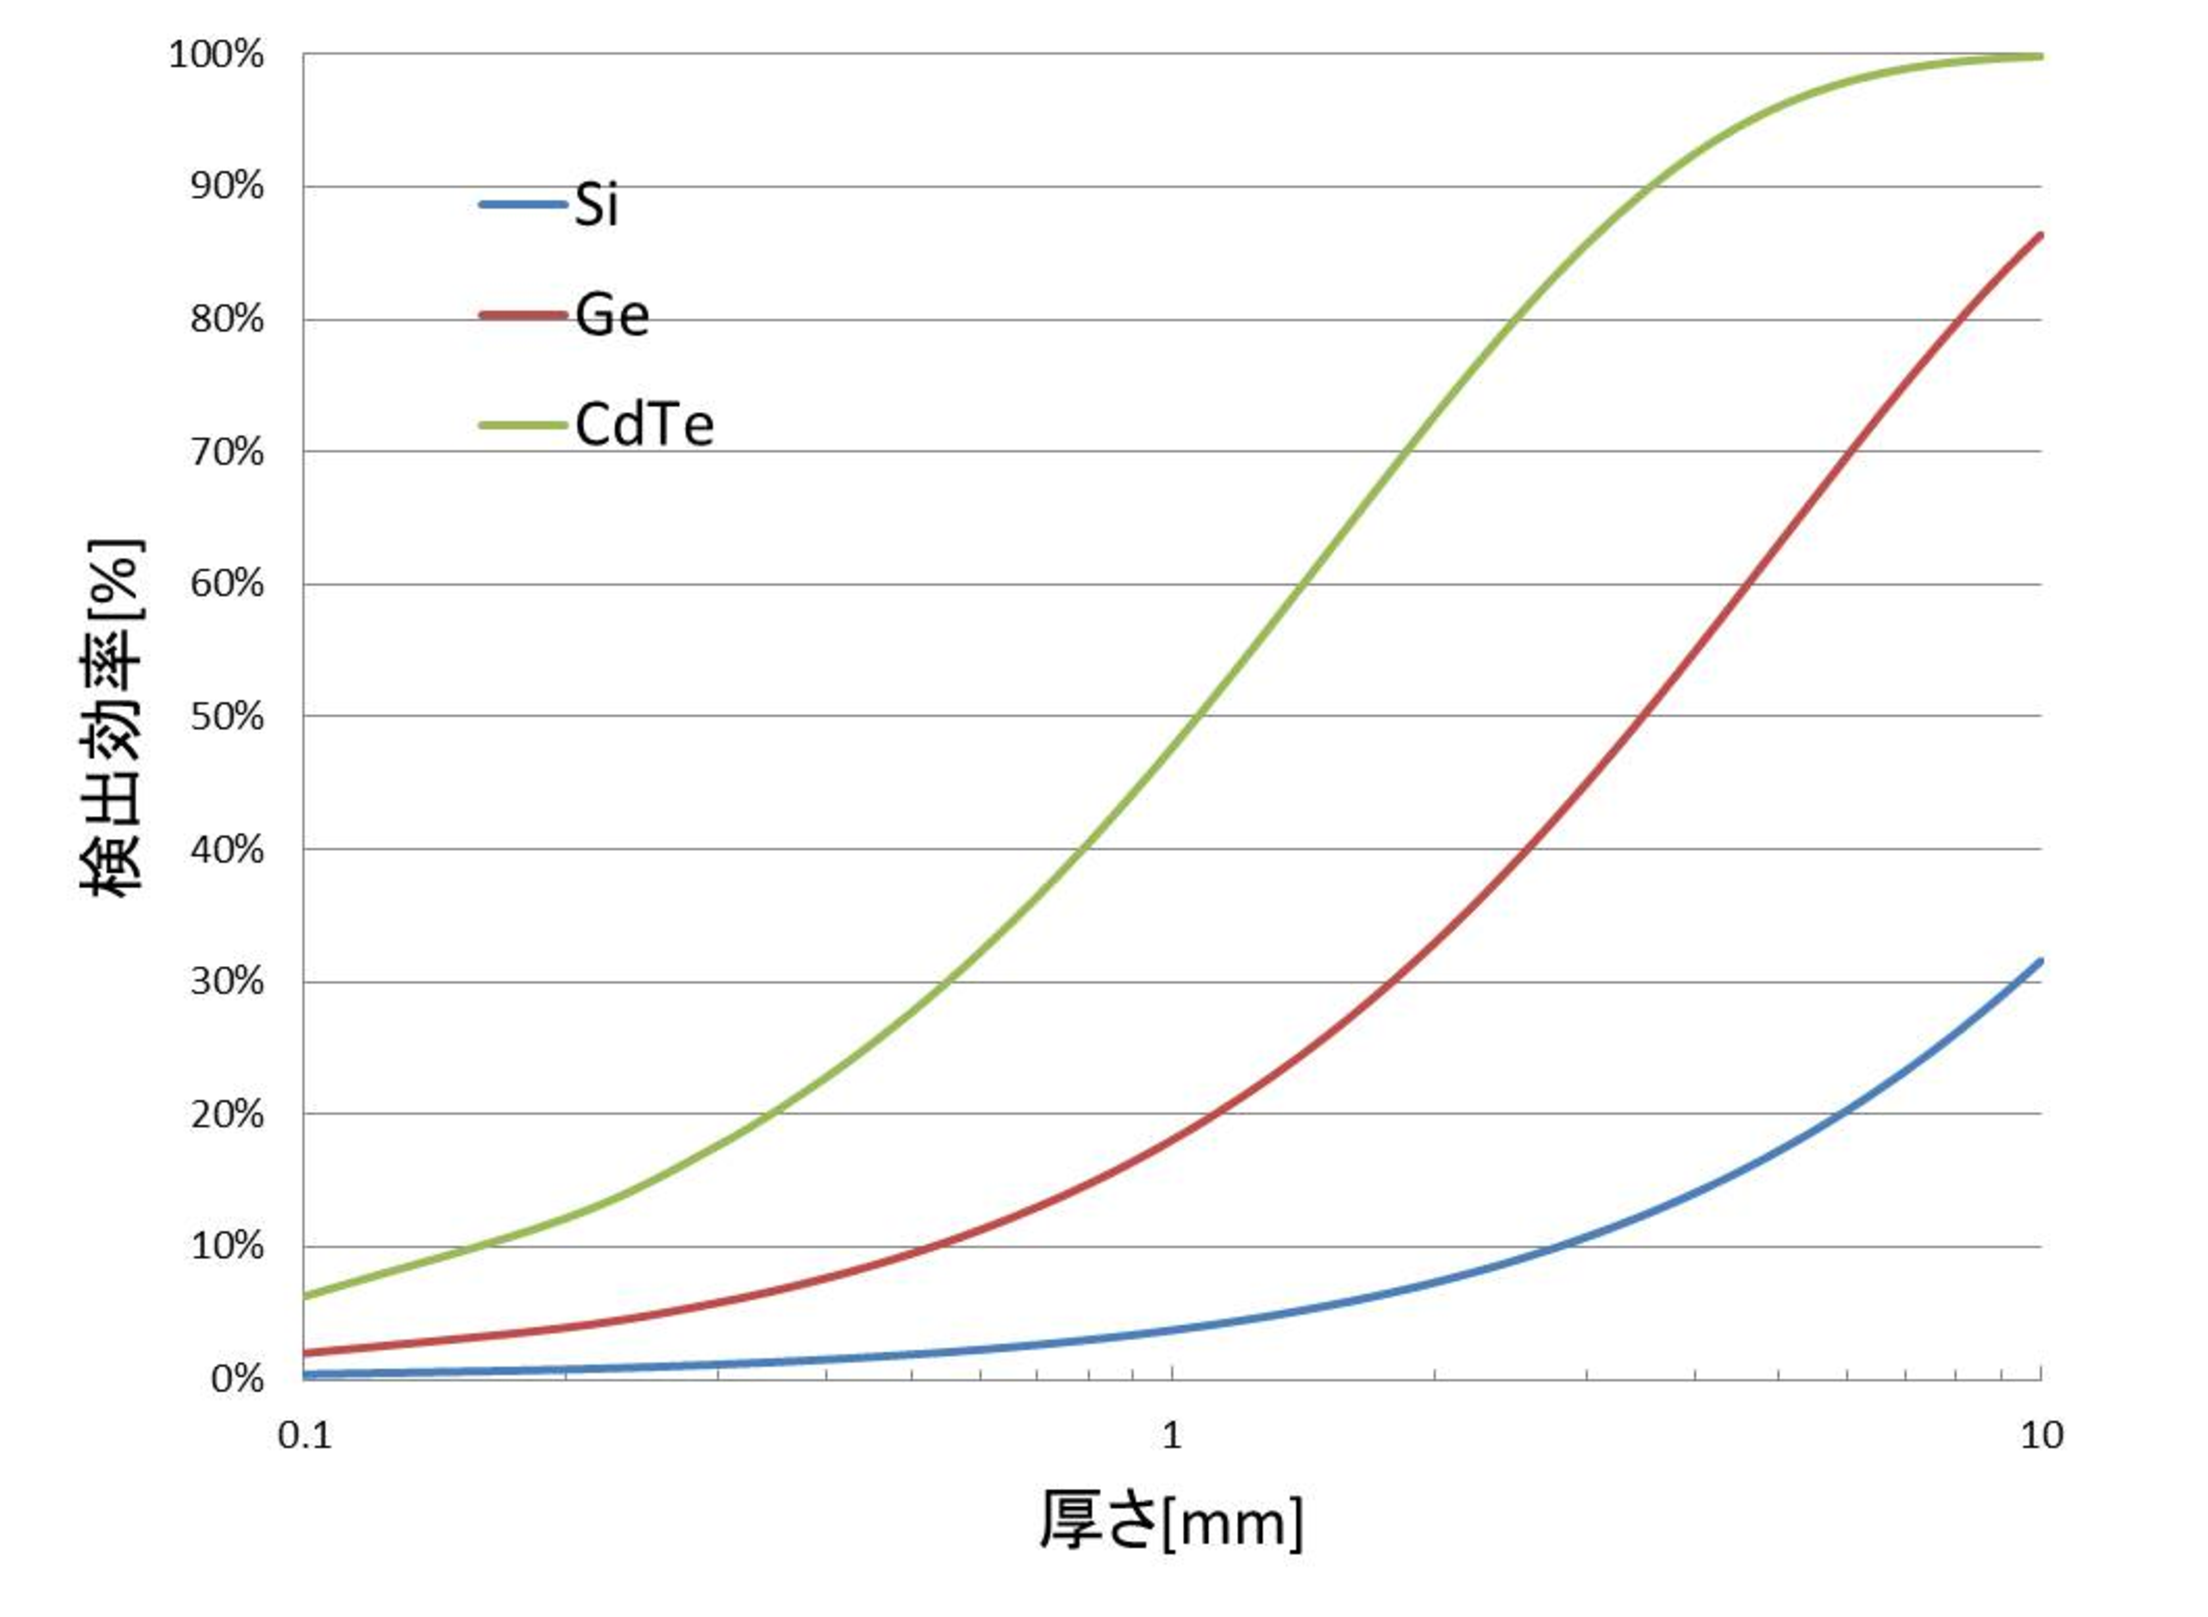
\includegraphics[width=8cm]{image/other/PDE_122.eps}
 \end{center}
  \end{minipage}
 \caption{Si,Ge,CdTeの60keV(左),120keV(右)に対する検出効率[NIST\cite{nist}より作成]}
 \label{fig:efficiency}
\end{figure}

\begin{figure}[H]
 \begin{center}
 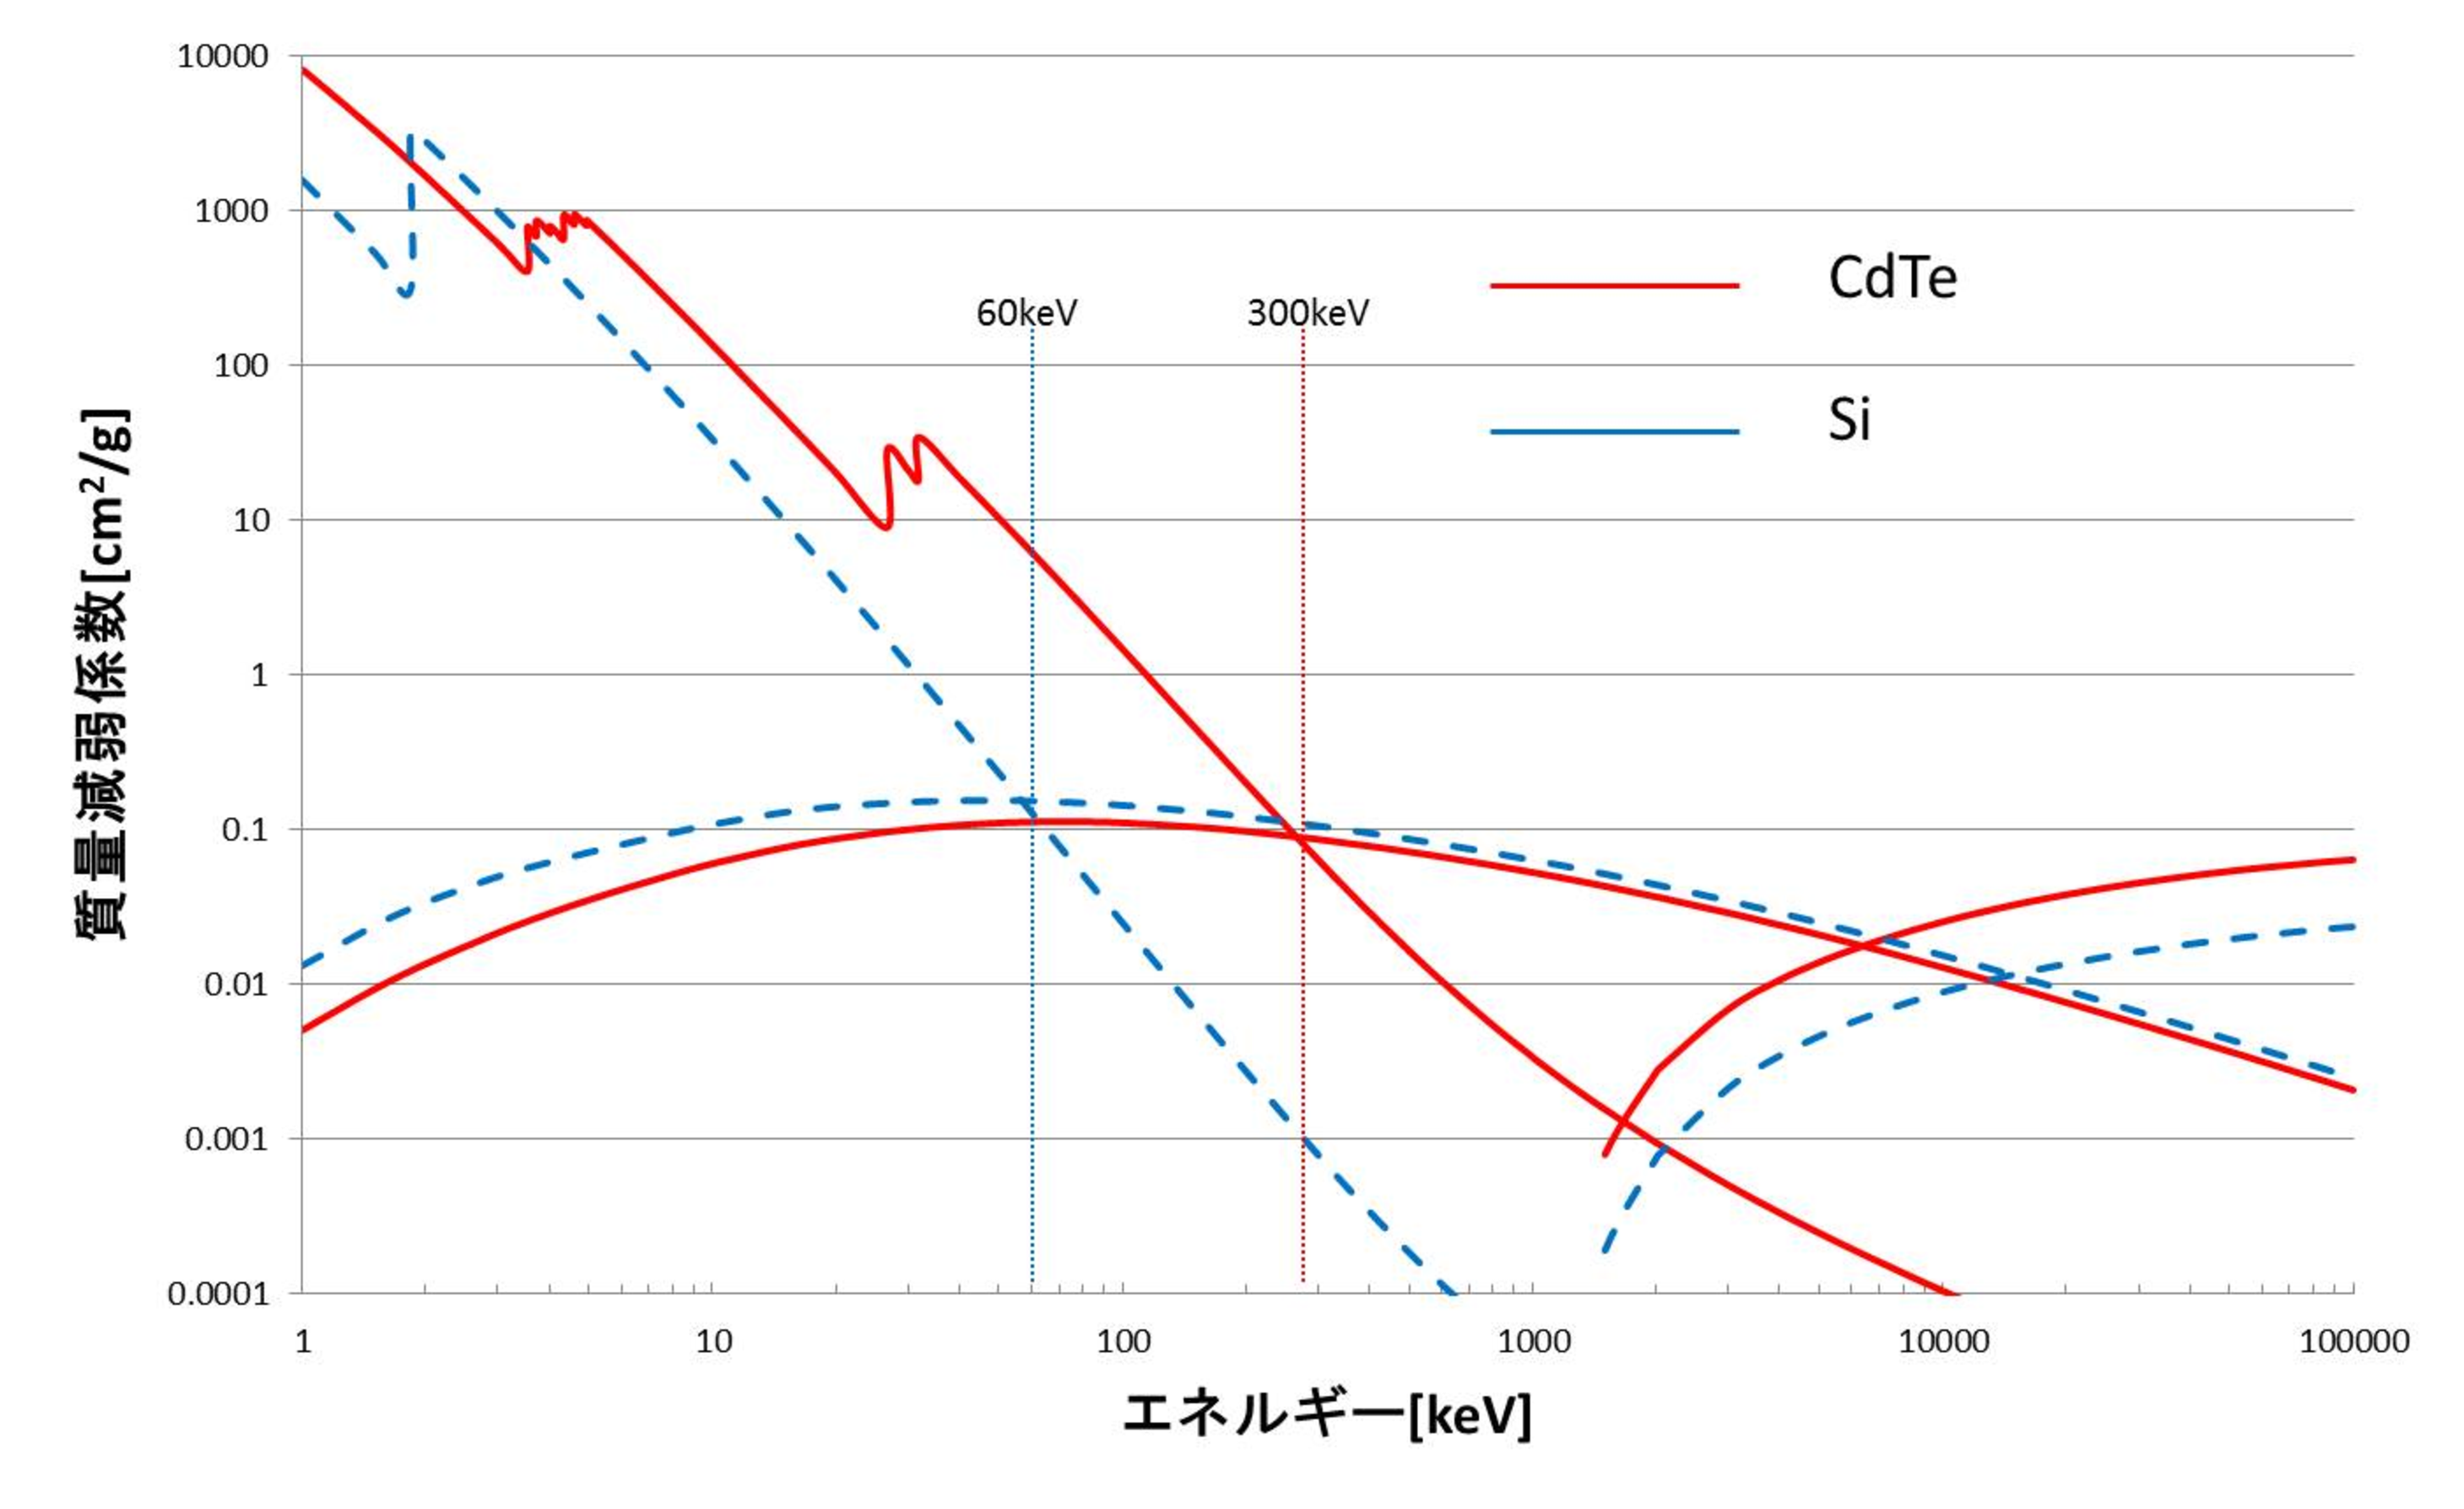
\includegraphics[width=10cm]{image/other/CdTe_Si.eps}
 \end{center}
 \caption{Si,Ge,CdTeに対する光子の光電吸収,コンプトン散乱,電子対生成による質量減弱係数[NIST\cite{nist}より作成]}
 \label{fig:liner_comp}
\end{figure}

\Fref{fig:efficiency}よりCdTeでは60keVのガンマ線に対しては1mmもあればほぼ100$\%$検出できるがSiでは1mmにおいては$7\%$程度しか検出できず,厚みを10mmにしてやっと約$50\%$検出できるようになる。また\Fref{fig:liner_comp}より高エネルギーにわたって光電効果が支配的であることが分かり,光電効果とコンプトン散乱の線源弱係数が等しくなるのはSiでは60keV,Geでは150keVであるのに対し,CdTeでは300keVで等しくなる。\\
\ \ 化合物半導体では,現存する最高の生成法を用いてもなお極く微量の不純物がな残存し,それらは電気的に活性なドーパントとして振舞う。例えば,アクセプタ準位を形成する不純物は材料を少しp型にし,その比抵抗を下げる。そこでバンドギャップ内に深いエネルギー準位を作る深いドナーを混ぜると,その補償作用により比抵抗を非常に大きくすることができる。同様の過程として,少しn型の材料の場合には深い準位を作る深いアクセプタを加える。こうした深いドナーやアクセプタは電荷キャリアの捕獲場所として働くため電荷キャリアの輸送を妨害する。この製法によりCdTeは非常に高い比抵抗($10^9\Omega$m)を持つようになる。

\section{CdTe半導体検出器の原理}

Siでは比抵抗が小さいので高電圧を印加した時のリーク電流が発生する。それを防ぐためpn接合によって比抵抗の高い空乏層を形成し,それを逆バイアスをかけて広げ有感層として用いたが,CdTeでは高い比抵抗を持つので結晶全体が有感層となり,結晶に電極(主に白金(Pt))をつけ単にバイアス電圧をかけることで検出器として用いることができる。この場合,CdTe検出器は固体電離箱として動作すると言える。

\section{CdTe半導体検出器の問題点}
CdTeは結晶全体が有感層となり,多くの電子正孔対を発生するが,先述したように深いドナーやアクセプタによって電荷キャリアの輸送が妨害されるので,電荷キャリア特に正孔の移動度($\mu_h$)が小さく,寿命($\tau_h$)が短いということが問題である。\Tref{semi_chara}に示してあるが$\mu\tau$は電子,正孔においてSi,Geよりも小さく,CdTeの厚さが2mm程度の場合,電荷収集時間は$>500$nsとなる。そのためSi やGeでは生じた電荷を損なうことなく集めることができたが,CdTe では,途中で生じた電荷を損なってしまうのでCdTeを小型にせざるを得ない。また低い$\mu\tau$によりパルス波高が電子正孔対の生成に位置によって異なり,スペクトルは低エネルギー側にテールを引いた形となり,エネルギー分解能はSi,Geよりも悪くなる。スペクトルのテールを低減するために高いバイアス電圧をかける必要がある。\\
\ \ しかし,スペクトルの情報が必要でない場合はCdTe検出器は寸法が非常にコンパクトで高い検出効率が得られるので,多くの分野における単純な計数にうまく利用されている。
%また,CdTe検出器は高ガンマ線束の下で電流モードで使われる。
%市販されているCdTe検出器は直径が1mmから1cmを少し超えるものまであり,厚さは2\UTF{FF5E}3mmかそれ以下に限られる。

%
\if0

\section{CdTe半導体を用いたピクセル検出器}
CdTeピクセル検出器とはX線やガンマ線の入った位置を検出し,撮像ができるようにしたものであり,その構造は\Fref{fig:pixel_CdTe}のように片側の電極を分割しピクセル化した構造になっている。それぞれのピクセル電極からの信号を一つ一つ別々のCSA,Shaping\ Ampで処理している。そのため読み出しチャンネル数は膨大になる。

\begin{figure}[H]
 \begin{center}
 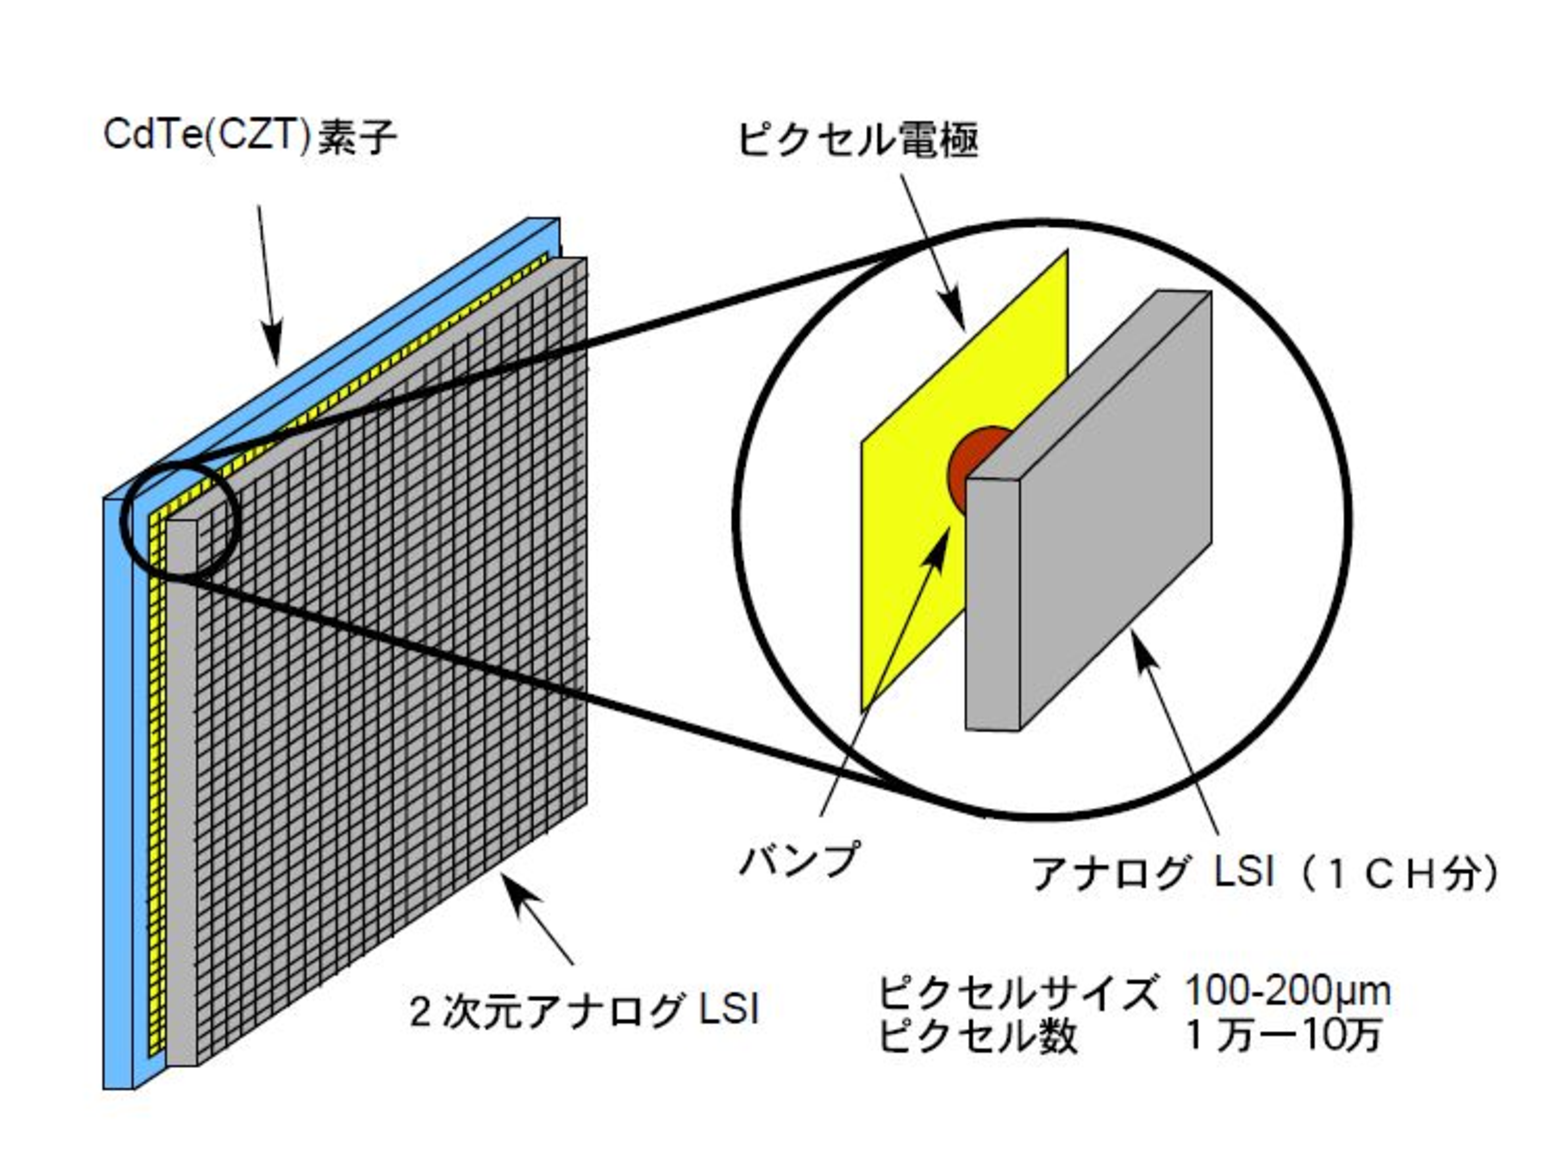
\includegraphics[width=10cm]{image/other/CdTe_pixel.eps}
 \end{center}
 \caption{CdTeピクセル検出器\cite{takahashi}}
 \label{fig:pixel_CdTe}
\end{figure}

%
\fi


	% 本文3
\chapter{X線CT}



\section{X線CTとは}
\begin{wrapfigure}{r}{90mm}
 \begin{center}
 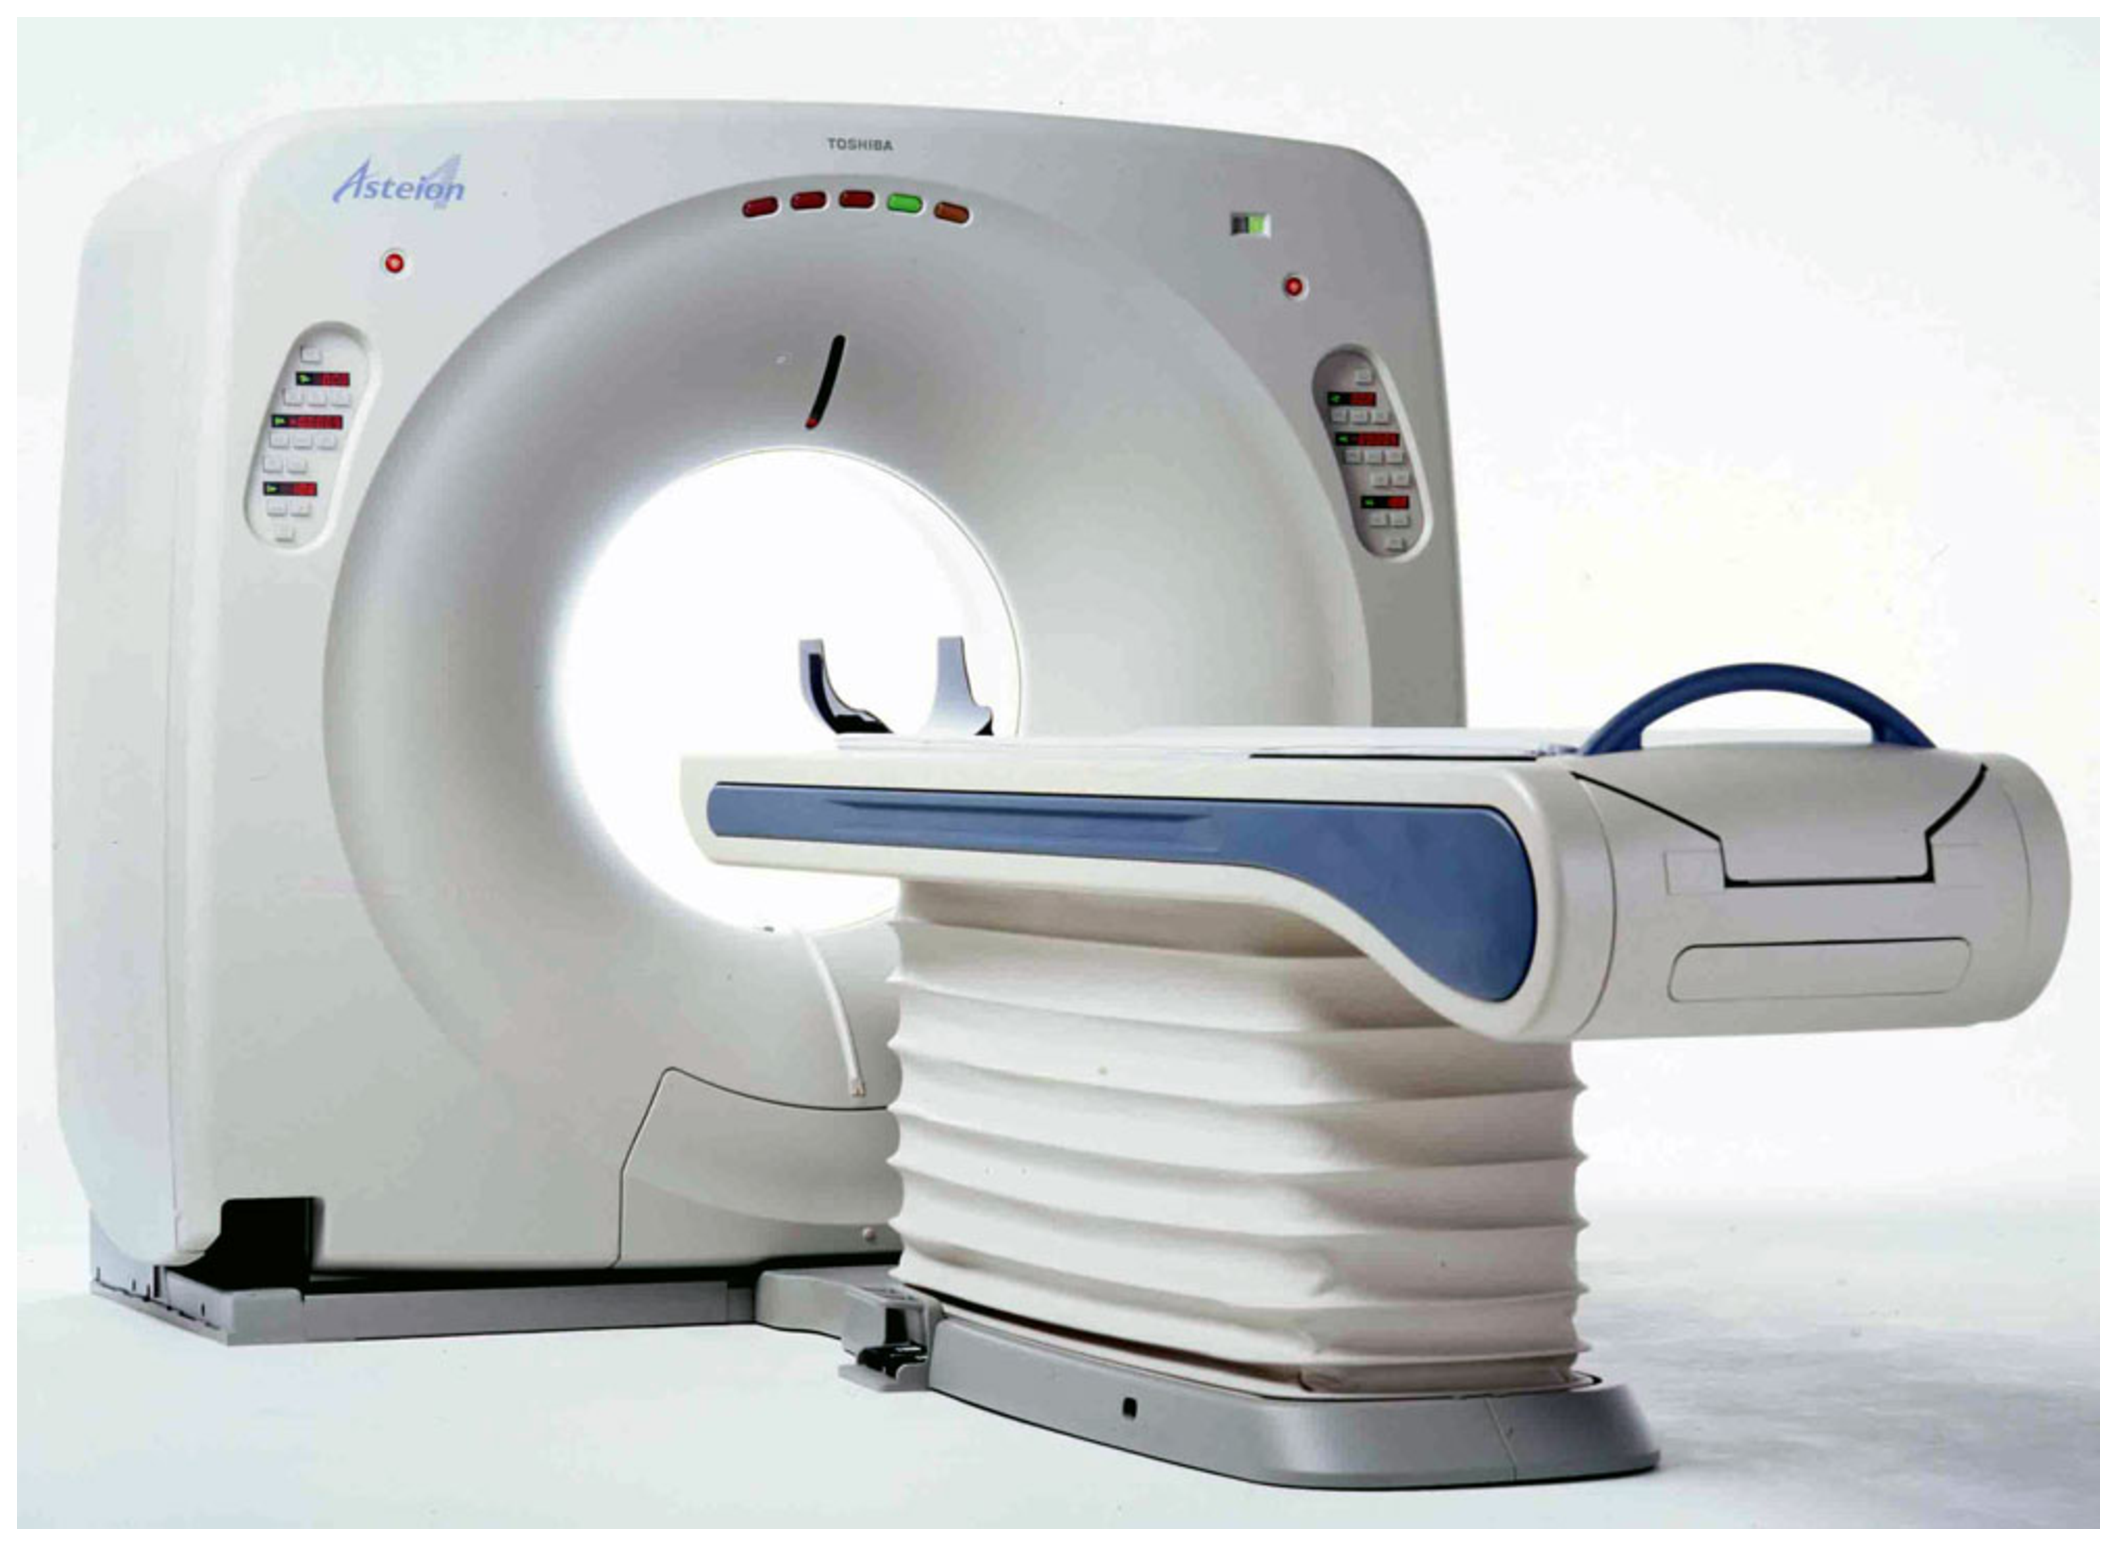
\includegraphics[width=8cm]{image/other/CT_toshiba.eps}
 \end{center}
 \caption{CT装置の外観}
 \label{fig:CT_toshiba}
\end{wrapfigure}
CTとはcomputed\ tomographyの略であり,日本語名称はコンピュータ断層撮影装置である。\Fref{fig:CT_toshiba}が典型的なCTの外観例である。X線管から連続エネルギースペクトルを持つX線が照射され,直進しながら物体中で減弱し,反対側にある検出器で減弱したX線の透過強度分布を測定する。そして,測定した透過強度分布から,X線の通しにくさを影絵にしたような投影データを取得する。この投影データをX線管と検出器を物体周りに回転して物体の多方向から取得し,フーリエ変換を用いて画像再構成し線減弱係数$\mu$の分布図としてCT画像を表示している。CT画像においては線源弱係数の高い組織は白く,線源弱係数の低し組織は黒く表示するのが慣例である。CTの方式には種々の方式があるが現在最も一般的なのは第三世代のファンビームを照射するX線源とそれに対向したX線検出器が被写体の周りを回るRotate/Rotate(R/R)方式であり,X線検出素子の数(チャンネル数)は現在は700-900程度になっており一回転のスキャン時間は0.3秒前後に達している。\\


\ \ 現在実用化されているCTの仕様の一例を\Tref{CT_philips}に示す。解像度は$\sim$0.2mm,画像を取得するのに要する時間は100ミリ秒台である。
\begin{table}[H]
\begin{center}
\begin{tabular}{cc} \hline
項目 & 仕様 \\\hline
フレームレート & 10,000 frame/sesc($\sim$120,000pixel/frame) \\
動作モード & 電流モード(エネルギー積分型) \\
シンチレータ & GOS($\sim$50,000ph/MeV) \\
解像度 & $\sim$2.4lp/mm($\sim$0.210mm) \\
リーク電流 & $<3$pA \\\hline
\end{tabular}
\end{center}
\caption{PHILIPS市販されているCTの仕様\cite{philips}}
\label{CT_philips}
\end{table}



\section{X線CTの検出器}
CTのX線検出器にシンチレータとフォトダイオード(PD)が用いられ、シンチレータでX線を光に変換し、PDで光電変換を行うのが最も主流である。シンチレータにはX線阻止能が高く、発光量が大きく、残光が少ないGOSが用いられる。また、R/R方式においては検出器全面に高さ20-30mmの主にタングステンなどの重金属でできている散乱線カット用のコリメータが配備されている。\Fref{fig:colimater}。

\begin{figure}[H]
 \begin{center}
 \includegraphics[bb=0.000000 0.000000 600.000000 622.00000,width=0.6\hsize]{image2/chapter5/colimater.png} 
 \end{center}
 \caption{CTの検出器の構造}
 \label{fig:colimater}
\end{figure}

また、PDからの出力電流をサンプリング時間(1ビューの時間、つまり0.2$\sim$1 ms)について積分し、たまった電荷量をA-D変換しディジタルデータとして送り出すDAS(Data Acquisition System)の構成の一例を\Fref{fig:DAS}に示す。

\begin{figure}[H]
 \begin{center}
 \includegraphics[bb=0.000000 0.000000 1000.000000 847.000000,width=0.6\hsize]{image2/chapter5/DAS.png} 
 \end{center}
 \caption{CTのDASの例。(少数のADCで全検出素子を分担する構成例)}
 \label{fig:DAS}
\end{figure}


DASに求めらる性能は以下のようなものがある。
\begin{enumerate}
\item サンプリング時間(0.2$\sim$1 ms)内に全検出素子の出力をA-D変換する高速性。
\item 検出器・DAS系の回路ノイズと量子化誤差はX線量子の統計的変動より十分低いレベルでなければならない
\item 被写体による減弱がない場合でも簡単にオーバーフローしない広いダイナミックレンジを持つ。
\end{enumerate}



また,CTの動作モードには電流モード(X線フォトンによって生成した電荷を所定時間蓄積し,電流信号を出力する方式)とパルス読み出し(X線フォトンを個々に計数するフォトンカウンティングモード)の2種類に大別されるが通常のCTは電流モード読み出しでありエネルギー積分型と呼ばれる。





\section{画像再構成原理}
現在のX線CTのX線管からはファンビームのX線が照射されるのが一般的であるが,ここでは簡単のため直線のX線ビームを用いて画像再構成原理を説明する(\Fref{fig:FBP})。

\begin{wrapfigure}{l}{60mm}
 \begin{center}
 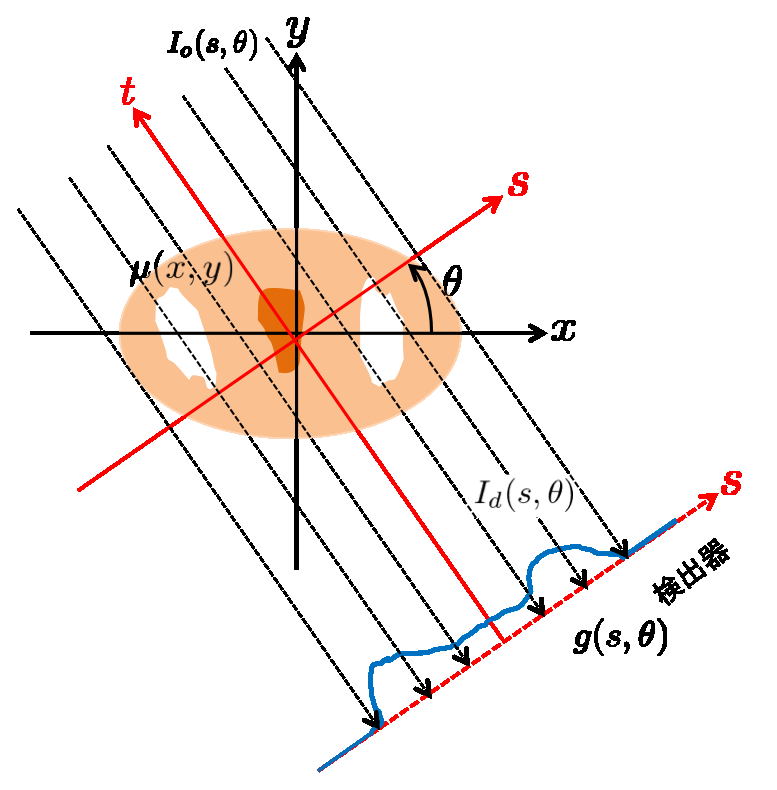
\includegraphics[width=6cm]{image/other/FBP.eps}
 \end{center}
 \caption{CTの画像再構成法の原理}
 \label{fig:FBP}
\end{wrapfigure}

最終的な目標は線源弱係数の分布$\mu(x,y)$を求めることである。\Fref{fig:FBP}において原画像$\mu(x,y)$と、計測データである投影データ$g(s,\theta)$の関係は次式のように定義される。
\begin{align}
g(s,\theta)&=\int^{\infty}_{-\infty}\mu(x,y)dt\\
&=\int^{\infty}_{-\infty}\int^{\infty}_{-\infty}\mu(x,y)\delta(x\cos{\theta}+y\sin{\theta}-s)dxdy\label{eq:radon}
\end{align}
ここで、$(x,y)$は被写体を固定した静止座標系、$(s,t)$は被写体周りを回転する検出器の座標系である。$s$は中央にある検出器を中心とし底からの位置、$t$は検出器に垂直な直線上にある被写体の位置を示す。\Eref{eq:radon}は原画像のうち回転座標系の$s$に相当する部分のみをデルタ関数によって抽出し、抽出された値の総和をとることを示す。これは角度$\theta(0\leq\theta<\pi)$に置いて位置$s$に相当する直線上で$\mu(x,y)$を線積分することに相当する。$g(s,\theta)$を横軸$s$,縦軸$\theta$として2次元画像で示したものがサイノグラムである。また各$\theta$と$t$で規定される投影データ1本1本をレイ(ray)という。また一つの角度方向のレイの1セットをビュー(view)という。\\
ここで入射光子数を$I_o$とし、人体との相互作用を受けずにそのまま透過した光子数を$I_d$とすれば次式が成り立つ。

\begin{align}
I_d(s,\theta)&=I_o(s,\theta)\exp{\left[-\int^{\infty}_{-\infty}\mu(x,y)dt\right]}\\
&=I_0(t,\theta)\exp[-g(s,\theta)]\\
∴g(&s,\theta)=-\ln\left[\frac{I_d(s,\theta)}{I_o(s,\theta)}\right]\label{eq:touei}
\end{align}
つまり,投影データ$g(s,\theta)$を入射強度$I_o$と検出器で受ける強度$I_d$から求めることができれば,その逆変換として,$\mu(x,y)$を求めることができる。そこで$\mu(x,y)$の二次元フーリエ変換$\hat{\mu}(\xi,\eta)$を考えると

\begin{align}
\hat{\mu}(\xi,\eta)=\displaystyle\int^{\infty}_{-\infty}\int^{\infty}_{-\infty}\mu(x,y)e^{-i2\pi(\xi x+\eta y)}dxdy
\end{align}となり,$(\xi,\eta)$を$\xi=\rho\cos{\theta},\eta=\rho\sin{\theta}$なる変換を行い,極座標系$(\rho,\theta)$に変換すると,

\begin{align}
\hat{\mu}(\rho\cos{\theta},\rho\sin{\theta})&=\int^{\infty}_{-\infty}\int^{\infty}_{-\infty}\mu(x,y)e^{-i2\pi\rho(x\cos{\theta}+y\sin{\theta})}dxdy\\&=\int^{\infty}_{-\infty}\int^{\infty}_{-\infty}\mu(x,y)e^{-i2\pi\rho s}dsdt\\
&=\int^{\infty}_{-\infty}\left[\int^{\infty}_{-\infty}\mu(x,y)dt\right]e^{-i2\pi\rho s}ds\\
&=\int^{\infty}_{-\infty}g(s,\theta)e^{-i2\pi\rho s}ds\\\label{eq:mu_hat}
&\equiv P(\rho,\theta)
\end{align}
つまり\Eref{eq:mu_hat}はある角度$\theta$における投影データを$s$について一次元フーリエ変換したものは線減弱係数$\mu$の二次元フーリエ変換の$\theta$成分である。よって,投影データを$\theta$が0から$\pi$に対して$\theta$方向\footnote{平行ビームであれば$p(t,\theta+\pi)=p(-t,\theta)$なので半回転で投影データの情報完備となる。画像の安定化のためには1回フルスキャンが基本だが,理論の説明は半回転の方がつ都合がよい。}の成分を得てそれらをtに関して1次元フーリエ変換することにより,$\mu(x,y)$のフーリエ空間$\hat{\mu}(\xi,\eta)$をタイヤのスポーク状に埋めることにより$\hat{\mu}(\xi,\eta)$が求まることになる。よって線源弱係数の分布$\mu(x,y)$は\Eref{eq:mu_hat}を逆フーリエ変換すればよいので
\begin{align}
\mu(x,y)&= \int^{\infty}_{-\infty}\int^{\infty}_{-\infty}\hat{\mu}(\xi,\eta)e^{i2\pi(\xi x+\eta y)}d\xi d\eta\\
&= \int^{2\pi}_{0}\int^{\infty}_{0}\hat{\mu}(\rho\cos{\theta},\rho\sin{\theta})e^{i2\pi\rho(x\cos{\theta} +y\sin{\theta} )} \displaystyle\left|
    \begin{array}{cc}
      \displaystyle\frac{\partial \xi}{\partial \rho} &  \displaystyle\frac{\partial \xi}{\partial \theta}  \\
      \displaystyle\frac{\partial \eta}{\partial \rho}  &  \displaystyle\frac{\partial \eta}{\partial \theta} 
    \end{array}
  \right|d\rho d\theta\\
  &= \int^{2\pi}_{0}\int^{\infty}_{0}\hat{\mu}(\rho\cos{\theta},\rho\sin{\theta})e^{i2\pi\rho(x\cos{\theta} +y\sin{\theta} )} \rho d\rho d\theta\\
  &= \int^{\pi}_{0}\int^{\infty}_{0}\hat{\mu}(\rho\cos{\theta},\rho\sin{\theta})|\rho|e^{i2\pi\rho(x\cos{\theta} +y\sin{\theta} )}  d\rho d\theta\\
    &= \int^{\pi}_{0}\left\{\int^{\infty}_{0}P(\rho,\theta)|\rho|e^{i2\pi\rho s}  d\rho\right\} d\theta\label{eq:FBP_end}
\end{align}
と求まる。\Eref{eq:FBP_end}は投影データを一次元フーリエ変換し、\Fref{fig:ramp}のように空間周波数の絶対値で示される高周波数強調フィルタのランプ(ramp)フィルタ$|\rho|$を掛けた後に。一次元フーリエ逆変換を行い実空間に戻す。フィルタ補正した投影データを$\theta(0\leq\theta<\pi)$について逆投影し原画像$\mu(x,y)$を得る。フィルターの種類はいくつかあるが代表的な二つのフィルターを\Fref{fig:filter}にあげる。

\begin{figure}[H]
 \begin{center}
 \includegraphics[bb=0.000000 0.000000 600.000000 327.000000,width=1\hsize]{image2/chapter5/filter.png} 
 \end{center}
 \caption{CTの画像再構成用いられるフィルター}
 \label{fig:filter}
\end{figure}
Rampフィルターは分解能に優れるがノイズを増強する。一方、Shepp-LogenフィルターはRampフィルターに比較しノイズを抑制するが解像度は劣る。またCT画像の画素の値(CT値)はこの線源弱係数を用いて以下のように定義されている。

\begin{align}
\rm CT値=1000\times\frac{\mu-\mu_w}{\mu_w}\label{eq:CT_value}
\end{align}
ここでCT値の単位はHU(Hounsfield\ unit)であり,$\mu_w$は水の線源弱係数である。しかし,$\mu$も$\mu_w$もX線質に依存する量であり,混合エネルギーX線を用いているため,物質を透過するとX線質は変化するのでCT値は完全な定量的な値ではない。様々な物質のCT値の目安を\Fref{fig:CT_value}に示す。

\begin{figure}[H]
 \begin{center}
 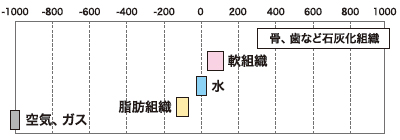
\includegraphics[bb=0.000000 0.000000 400.000000 140.000000,width=0.8\hsize]{image2/chapter1/CT_value.jpg} 
 \end{center}
 \caption{様々な物質のCT値}
 \label{fig:CT_value}
\end{figure}


\section{CTの画質評価}
CTの画質評価に主にどれくらい画像ノイズ評価、どれくらい細いものが見えるかという空間分解能表、CT値が近い物質をどれくらい区別できるかという低コントラスト分解能評価お3つが主にある。

\subsection{画像ノイズ評価\label{sec:noise}}
X線CTで水ファントムのような一様な被写体を撮影した場合、その物質の線減弱係数$\mu$に従って、各ピクセルのCT値は一様に等しく計算されるはずである。しかし、実際は諸因子に由来する統計的な変動(揺らぎ)によってCT値はばらついて一定とならず、この揺らぎ成分を一般的に画像ノイズと呼ぶ。この画像ノイズは直感的にも推察されるように投影データのノイズの比例する。ここでは投影データのノイズはX線量子の統計的変動が支配的である。X線量子の統計的変動とは次のようなものである。完全な計測系を用いて到来フォロン数の計測を繰り返しても、結果は毎回異なる。個々のX線フォトンが被写体内で減弱していくプロセスは確率現象であるためであり、一般的にポアソン分布に従うと仮定される。各回のフォトン数計測値が$N$個であるとし、平均して$\langle N \rangle$個が計測されたとする。$N$は$\langle N \rangle$を中心に誤差$\varepsilon_N$でばらつくが、この$\varepsilon_N$がX線量子の統計的変動である。$\varepsilon_N$の標準偏差を$\sigma_N$とすれば、ポアソン分布を仮定しているので$\sigma_N=\sqrt{\langle N \rangle}$である。誤差のない測定系であっても計測データのS/N比はX線量子の統計的変動で決まる物理限界$\langle N \rangle/\sigma_N=\sqrt{\langle N \rangle}$を超えることはできない。\\
ここで、検出器・DASは完璧でなくノイズ$\varepsilon_d$を伴うが、その場合の投影データのノイズレベルを求めてみる。CTのX線計測は様々なエネルギーの混じった混合エネルギースペクトルの多色X線の吸収線量計測であるが、ここでは簡単のためにフォトンカウンティングモードでの計測であるとする。被写体へ入射X線フォトン数を$N_{\rm in}$とする。\Eref{eq:touei}よりノイズがなければ投影データの値は
\begin{align}
p_{\rm ideal}&=-\ln{\left(\frac{N}{N_{\rm in}}\right)}\\
&=-\ln{N}+\ln{N_{\rm in}}\\
&=-\ln{\langle N \rangle}+\ln{\langle N_{\rm in} \rangle}
\end{align}
ノイズがあるときの投影データは
\begin{align}
p_{\rm actual}&=-\ln{\left( \frac{N+\varepsilon_d}{N_{\rm in}}   \right)}\\
&=-\ln{(N+\varepsilon_d)}+\ln{N_{\rm in}}\\
&=-\ln{(\langle N \rangle + \varepsilon_N + \varepsilon_d)}+\ln{(\langle N_{\rm in} \rangle + \varepsilon_{\rm in})}
\end{align}
ここで、$\varepsilon_{\rm in}$は$N_{\rm in}$に含まれるX線量子の統計的変動でありその標準偏差は$\sqrt{\langle N_{\rm in} \rangle}$であるが、$N_{\rm in}$は被写体により減弱していない大きな値なので$\langle N_{\rm in} \rangle\gg|\varepsilon_{\rm in}|$であり、$\ln{\langle N_{\rm in} \rangle + \varepsilon_{\rm in}}\approx\ln{\langle N_{\rm in} \rangle}$と近似してよい。従って
\begin{align}
p_{\rm actual}&\approx-\ln{(\langle N \rangle + \varepsilon_N + \varepsilon_d)}+\ln{\langle N_{\rm in} \rangle}\\
&=-\ln\left\{\langle N \rangle\left(1+\frac{\varepsilon_N+\varepsilon_d}{\langle N \rangle} \right)\right\}+\ln{\langle N_{\rm in} \rangle}\\
&=-\ln{\langle N \rangle}-\ln\left(1+\frac{\varepsilon_N+\varepsilon_d}{\langle N \rangle} \right)+\ln{\langle N_{\rm in} \rangle}\\
\end{align}
ここで第ニ項を級数展開し$\langle N \rangle$に比べて$\varepsilon_N$と$\varepsilon_d$は十分小さいとして高次の項を落とすと、
\begin{align}
p_{\rm actual}&\approx-\ln{\langle N \rangle}-\frac{\varepsilon_N+\varepsilon_d}{\langle N \rangle}+\ln{\langle N_{\rm in} \rangle}\\
&=p_{\rm ideal} + \varepsilon_p
\end{align}
ここで
\begin{align}
\varepsilon_p\equiv-\frac{\varepsilon_N+\varepsilon_d}{\langle N \rangle}
\end{align}
と定義した。すなわち$p_{\rm actual}$は$p_{\rm ideal}$の周囲に誤差$\varepsilon_p$でばらつく。この$\varepsilon_p$の標準偏差$\sigma_p$を求める。ここで$\varepsilon_d$は平均値ゼロ、標準偏差$\sigma_d$とする。$\varepsilon_N$と$\varepsilon_d$とは互いに相関がないので分散の加算式より、

\begin{align}
\sigma^2_p&=\frac{\sigma^2_N+\sigma^2_d}{\langle N \rangle^2}\\
&=\frac{\langle N \rangle + \sigma^2_d}{\langle N \rangle^2}
\end{align}
従って
\begin{align}
\langle N \rangle\gg\sigma_dのとき\ \ \ \sigma_p\approx\frac{1}{\sqrt{\langle N \rangle}}\label{eq:normal}\\
\langle N \rangle\ll\sigma_dのとき\ \ \ \sigma_p\approx\frac{\sigma_d}{\sqrt{\langle N \rangle}}\label{eq:ijou}
\end{align}
\Eref{eq:normal}が通常の運用状態である。ここではX線量子の統計的変動だけが投影データ(すなわちCT画像の)ノイズ起源で画像ノイズは検出線量の平方根に反比例する。\\
\Eref{eq:ijou}のような状況では、画像ノイズは検出線量に反比例して変化する。これは一種の異常事態であり、大きな被写体であるにもかかわらず過度に照射線量を減らしたり薄いコリメーション幅とした場合には発生しうる。その場合、画像ノイズのみならず別種の画質問題も顕在化することがあり、診断に耐える画像は得られない。\\
X線量子の統計的変動に関与する要因は
\begin{enumerate}
\item 線質(管電圧)
\item 管電流
\item 撮影時間
\item ピッチ
\item detector configuration(colimation)
\end{enumerate}
があげられる。またX線量子の統計的変動が画像ノイズの最大要因であるが、画像再構成・画像処理(再構成スライス厚、再構成法、フィルタ関数)によっても画像ノイズは変動する。

\if0
%森田バージョン
X線CTで水ファントムのような一様な被写体を撮影した場合、その物質の線減弱係数$\mu$に従って、各ピクセルのCT値は一様に等しく計算されるはずである。しかし、実際は諸因子に由来する統計的な変動(揺らぎ)によってCT値はばらついて一定とならず、この揺らぎ成分を一般的に画像ノイズと呼ぶ。この画像ノイズは直感的にも推察されるように投影データのノイズの比例する。ここでは投影データのノイズはX線量子の統計的変動が支配的である。X線量子の統計的変動とは次のようなものである。完全な計測系を用いて到来フォロン数の計測を繰り返しても、結果は毎回異なる。個々のX線フォトンが被写体内で減弱していくプロセスは確率現象であるためであり、一般的にポアソン分布に従うと仮定される。各ピクセルの投影データの値は\Eref{eq:touei}から求められるが、X線量子の統計的変動によって$I_d/I_o$が揺らぎ、投影データの値も揺らぐことになる。極端な線量不足による電気系のノイズが顕在化する場合を除き、X線量子数を$n$とすると、投影データの値の揺らぎつまりピクセルごとのCT値の揺らぎ($SD$)は
\begin{align}
SD\propto\frac{1}{\sqrt{n}}
\end{align}

このように、CT値の変動はX線量子数の平方根に反比例し、このX線量子数は管電流時間積[mAs]または管電圧[kV]によって調整可能である。一般的にCT検査ではほとんどの場合、管電圧は120kVカラ140kVの一定の値あが使用されるため、管電流や撮影時間を調整することで画像ノイズをコントロールするこができる。
\fi


\subsection{空間分解能評価}
空間分解能とはどのくらい細いものを分離して認識できるかという識別限界を数値化したものである。CTにおける空間分解能は、高コントラスト分解能ファントムを用いて視覚的に評価する方法と、解像特性として定量的に変調伝達関数(Modulation Transfer Function: MTF)を測定する方法の2つが推奨されている。空間分解能を決定づける要因は以下のようなものがあげられる。
\begin{enumerate}
\item 焦点サイズと検出器サイズ
\item サンプリングピッチ
\item view数
\item 再構成FOV
\item 再構成関数
\item その他(架台振動、管球焦点移動なども影響がある。マルチスライスCTの登場により再構成方法も多様化し、これらの様々な要因によっても空間分解能が変化する。)
\end{enumerate}

\subsubsection*{高コントラスト分解能ファントムによる空間分解能評価}

\begin{wrapfigure}{r}{90mm}
 \begin{center}
 \includegraphics[bb=0 0 760 640,width=0.4\hsize]{image2/chapter5/high_contrast_phantom.png} 
 \end{center}
 \caption{高コントラスト分解能\\ファントムの例}
 \label{fig:high_contrast_phantom}
\end{wrapfigure}
一般的な評価ファントムとしては、\Fref{fig:high_contrast_phantom}のようにアクリル樹脂などの中に空気の穴(直径$d$)がピッチ$2d$で配列されたものが用いられる。これをCT撮影して再構成を行い画像上で$d$の穴が分離して見えるか見えないかという主観的な評価を行う。この評価においては定量性には欠けるが穴が細くなる、つまり入力信号の周波数が大きくなるにつれて応答性が次第に低下していることなどもわかる。例えば0.5mmの径であれば、空間周波数1.0 Lp/mmにおける応答を見ていることになる。下がって、それぞれの径に対応する空間周波数における応答を比較することができる。しかし、本法では空間周波数ごとの応答を定量的な数値で表すことはできず、本法で評価してるのは識別限界となる最高周波数のみである。



\subsubsection*{MTFによる空間分解能評価\label{sec:MTF}}
上述の高コントラスト分解能ファントムによる評価では、「どのくらい細いものを分離して認識できているか」という主観的な視覚評価であった。一方で変調伝達関数(Modulation Transfer Function: MTF)では「見える、見えない」といった主観的な要素はなう、また周波数領域について定量的、客観的に評価が行える。MTFとは入力信号に対して、出力信号が「どれだけボケたか」を周波数成分ごとに数値化したものである。MTFを求める入力信号としては、店信号を入力する点像強度分布(Point Spread Function : PSF)と線信号を入力する線像強度分(Line Spread Function : LSF)がある。ここでは最も一般的な手法であるワイヤ法という、スライス面と垂直に張ったごく細い金属ワイヤの断面をCTで撮像し、得られたPSFからMTFを求める手法について詳細に述べる。\\
PSFから求めるMTFとは「何もないところに突然ある限りなく0に近い幅で無限大のCT値を持つ入力信号」が「どのようにボケたのか」ということを示したものである。この場合の極めて特殊な入力信号をインパルス信号と呼ぶ。「どのようにボケたのか」ということを評価するために、ボケによって得られた分布すなわちPSFをフーリエ変換す流ことで周波数空間における応答値が得ることができる。インパルス波形を理想的なデルタ関数とすれば、これをフーリエ変換すると全周波数領域で大きさは1となる(\Fref{fig:delta})。デルタ関数を線形システムに入力したときの出力をインパルス応答という。システムを通過したときのボケにより広がった形状のインパルス応答をフーリエ変換したものが周波数応答関数であり、その絶対値がMTFである。\\

\begin{figure}[H]
 \begin{center}
 \includegraphics[bb=0.000000 0.000000 507.798022 196.303772,width=0.6\hsize]{image2/chapter5/delta.png} 
 \end{center}
 \caption{デルタ関数のフーリエ変換}
 \label{fig:delta}
\end{figure}

デルタ関数をフーリエ変換した時の全周波数領域での大きさが1であることから、広がった形状のインパルス応答をフーリエ変換して得られた応答値は、ボケによって低下したレベルや、微小構造描出のために特定の周波数を強調しているような状況が周波数成分ごとにその比率としてMTF上に示される。\\
CTに於いてはスライス面と垂直に張ったごく細いワイヤは、ワイヤのある位置においてX線がほとんど不透過であるので、線減弱係数は非常に大きくなる。よって、ワイヤーの径が非常に小さければ、それによって近似的な2次元のインパルス信号が得られ(\Fref{fig:inpulse}(左))、その信号がCTシステムによってボケを受けた出力信号がCT画像上に現れたワイヤの画像、すなわちPSFである(\Fref{fig:inpulse}(右))。このPSFを直接2次元フーリエ変換するか、LSFに変換して1次元フーリエ変換をsして周波数応答を求めるのがワイヤ法である。\Fref{fig:MTF_outou}は、3種類のLSFに対するMTFを示している。この図では、幅が狭く急峻なLSFほど高いMTFとなっており、直感的にもわかりやすい。この幅が狭くなり最後にインパルス信号そのものになれば、MTFは高周波成分まで1.0となり理想的な状態となる。

\begin{figure}[H]
 \begin{center}
 \includegraphics[bb=0 0 1000 893,width=1\hsize]{image2/chapter5/inpulse.png} 
 \end{center}
 \caption{インパル信号とインパル応答(PSF)およびそれぞれのMTF}
 \label{fig:inpulse}
\end{figure}

\begin{figure}[H]
 \begin{center}
 \includegraphics[bb=0 0 1000 323,width=1.0\hsize]{image2/chapter5/MTF_outou.png} 
 \end{center}
 \caption{各インパルス応答と対応するMTFの関係}
 \label{fig:MTF_outou}
\end{figure}

\if0
MTFの測定手順を\Fref{fig:MTF_method}に示す。

\begin{figure}[H]
 \begin{center}
 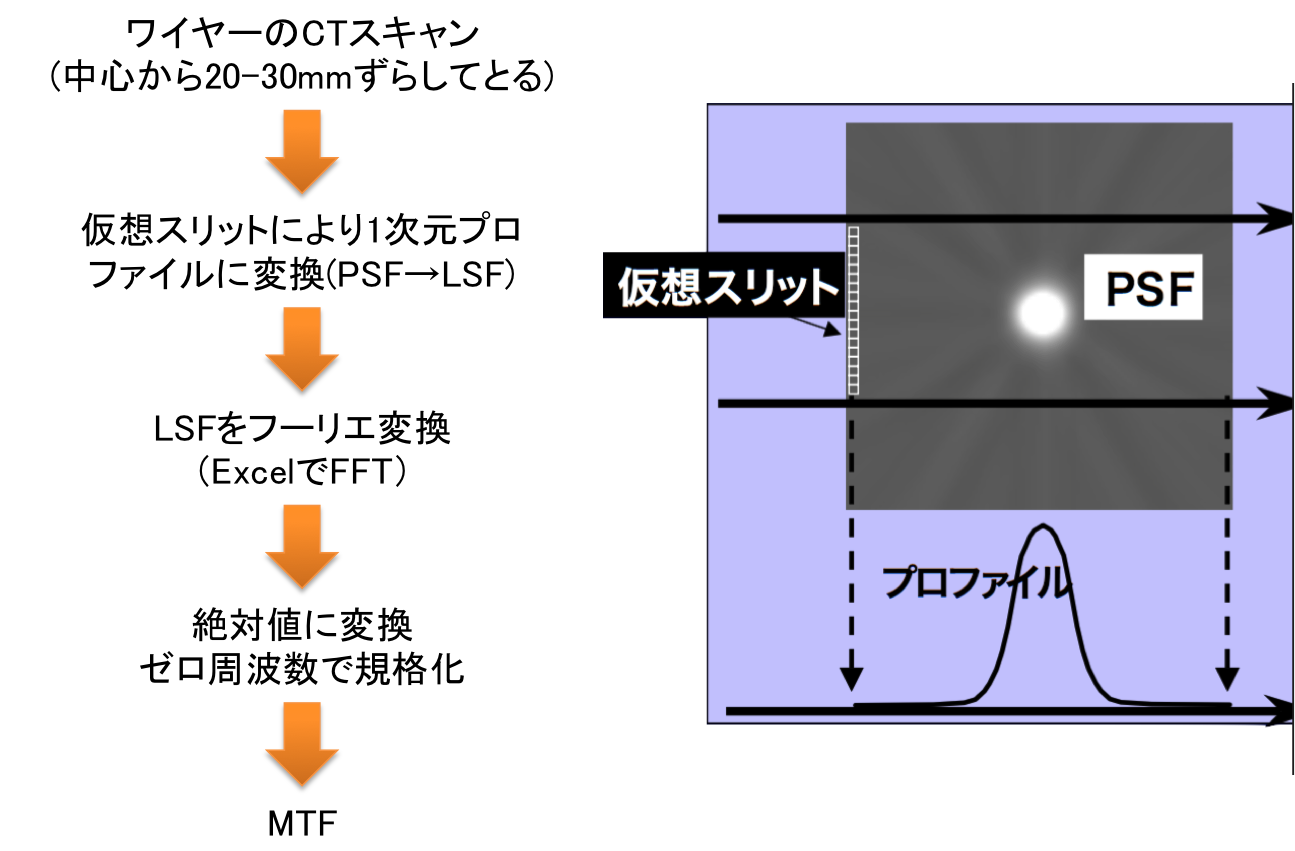
\includegraphics[bb=0.000000 0.000000 621.548619 408.446235,width=1\hsize]{image2/chapter5/MTF_method.png} 
 \end{center}
 \caption{MTFの測定手順}
 \label{fig:MTF_method}
\end{figure}
\fi

\subsection{低コントラスト分解能評価}
周囲と比べてCT値差が小さく、かつ寸法の小さな物体を描出する能力を低コントラスト分解能という。評価用ファントムとしては背景となる物質の中にそれとわずかにCT値が異なる組織の構造を埋め込んだものが用いられる。低コントラスト分解能は主にコントラスト値(どれだけ大きなコントラストをつけて描出できるか)と画像ノイズが支配的である。したがって、画像ノイズに影響する因子は全て低コントラスト分解能の因子でもある。低コントラスト分解能を定量的に評価するために一般的に対象物質のCT値$\mu_M$と背景のCT値$\mu_B$の差を背景の画像ノイズ$\sigma_B$で割った、CNR(Contrast-noise-ratio: CNR)という値が用いられる。
\begin{align}
CNR = \frac{\mu_M-\mu_B}{\sigma_B}
\end{align}
CNRが高ければ高いほど、CT値が近い物質を明確に区別できるということになる。

\section{従来のエネルギー積分型X線CTの問題点\label{sec:problem}}

第1章でも述べたがフォトダイオードの暗電流は 数十pA$\sim$数百pAであり、この暗電流に十分打ち克つ信号電流を検出器から出力する必要がある。CTの画質を律速しているのは「信号電流($I_s$)$\gg$暗電流($I_d$)」を実現することに他ならない。ここで従来のCTにおいて「$I_s\gg I_d$」を実現させるために必要な照射線量を概算してみる。被写体透過後のX線強度を$I_x$[/s]、PDの暗電流$I_d$を100[pA]とする。60keVのX線が従来一般的に用いられるGOSシンチレータ(40,000 ph/MeV)に検出されたとし、PDの量子効率を50\%すると、
\begin{align}
I_d&\gg I_s\\
60\time40\times0.5\times1.6\times10^{-19} [C] \times I_x&\gg100\times10^{-12}\\
I_x&\gg 5.2\times10^5
\end{align}
程度となる。また読み出し回路を通ることでさらにノイズが増大することを考えれば被写体を透過した時点で$10^{6}$cts/s/mm$^2$のレートが必要になる。人体透過後は線量は約1/1000になるので\footnote{人体を水と透過と考え60keVにおける水の線減弱係数は0.206[1/cm]、人体を30cmとすれば$e^{-\mu L}\sim1/1000$となる。}必要な照射線量は$10^{8-9}$cts/s/mm$^2$と膨大になる。このためX線CTによる医療被ばく量は膨大であり一回の撮影での被ばく量は10mSvにもおよぶ。また、このような超高線量下おいては様々なエネルギーの混ざった混合エネルギーのX線のそれぞれの反応パルスイベントを区別するのは困難であり、読み出し方法はある一定時間電荷を積分した電流モードである。そのため個々のX線光子のエネルギー情報は完全に失われてしまうため、得られる画像はCT値のみを一つのパラメーターとするモノクロ画像となってしまう。電流モードつまりエネルギー積分型に読み出していることにより以下の2つがCT誕生当初から問題となっていた。


\if0
先述のように,従来のX線CTでは透過X線の検出において,電流モードつまりX線フォトンによって生成した電荷を所定時間蓄積し,電流信号を出力する方式を用いている。そのため従来型X線CTは「エネルギー積分型」と呼ばれ,各エネルギーのX線光子がどれくらい透過してきたのかというエネルギー情報は失ってしまう。しかし,人体中の元素は低原子の組織が中心であるため,X線の減弱は原子番号に依存するコンプトン散乱が支配的であるため,混合エネルギーのX線は低・高エネルギーでもある物質中で一定の割合で減衰するため線質はあまり変化しない。したがって,透過物質の実効エネルギーに対する線源弱係数はある程度正確に求めることができる。そのため長年にわたって個々のX線光子のエネルギーの計測は行われなかった。しかし,以下に述べる2点がCT誕生時からの問題点として挙げられる。
\fi

\subsection{CT値が同一である物質の弁別が困難}
CT値は,物質の「質量減弱係数」と「密度」の積である線源弱係数により決定されることを述べた。質量減弱係数はX線エネルギーが一定であれば物質固有の値(\Fref{fig:atten}左)であるが,CT値を決定する線減弱係数は物質の密度にも依存するため,撮像対象物の密度状態によっては物質が異なっても(原子番号が異なっても)CT値が同一になってしまうことがある(\Fref{fig:atten}右)。通常のCTでは,CT値が唯一のパラメータであるため,物質の正確な弁別は困難と言える。

\begin{figure}[H]
 \begin{minipage}{0.52\hsize}
  \begin{center}
   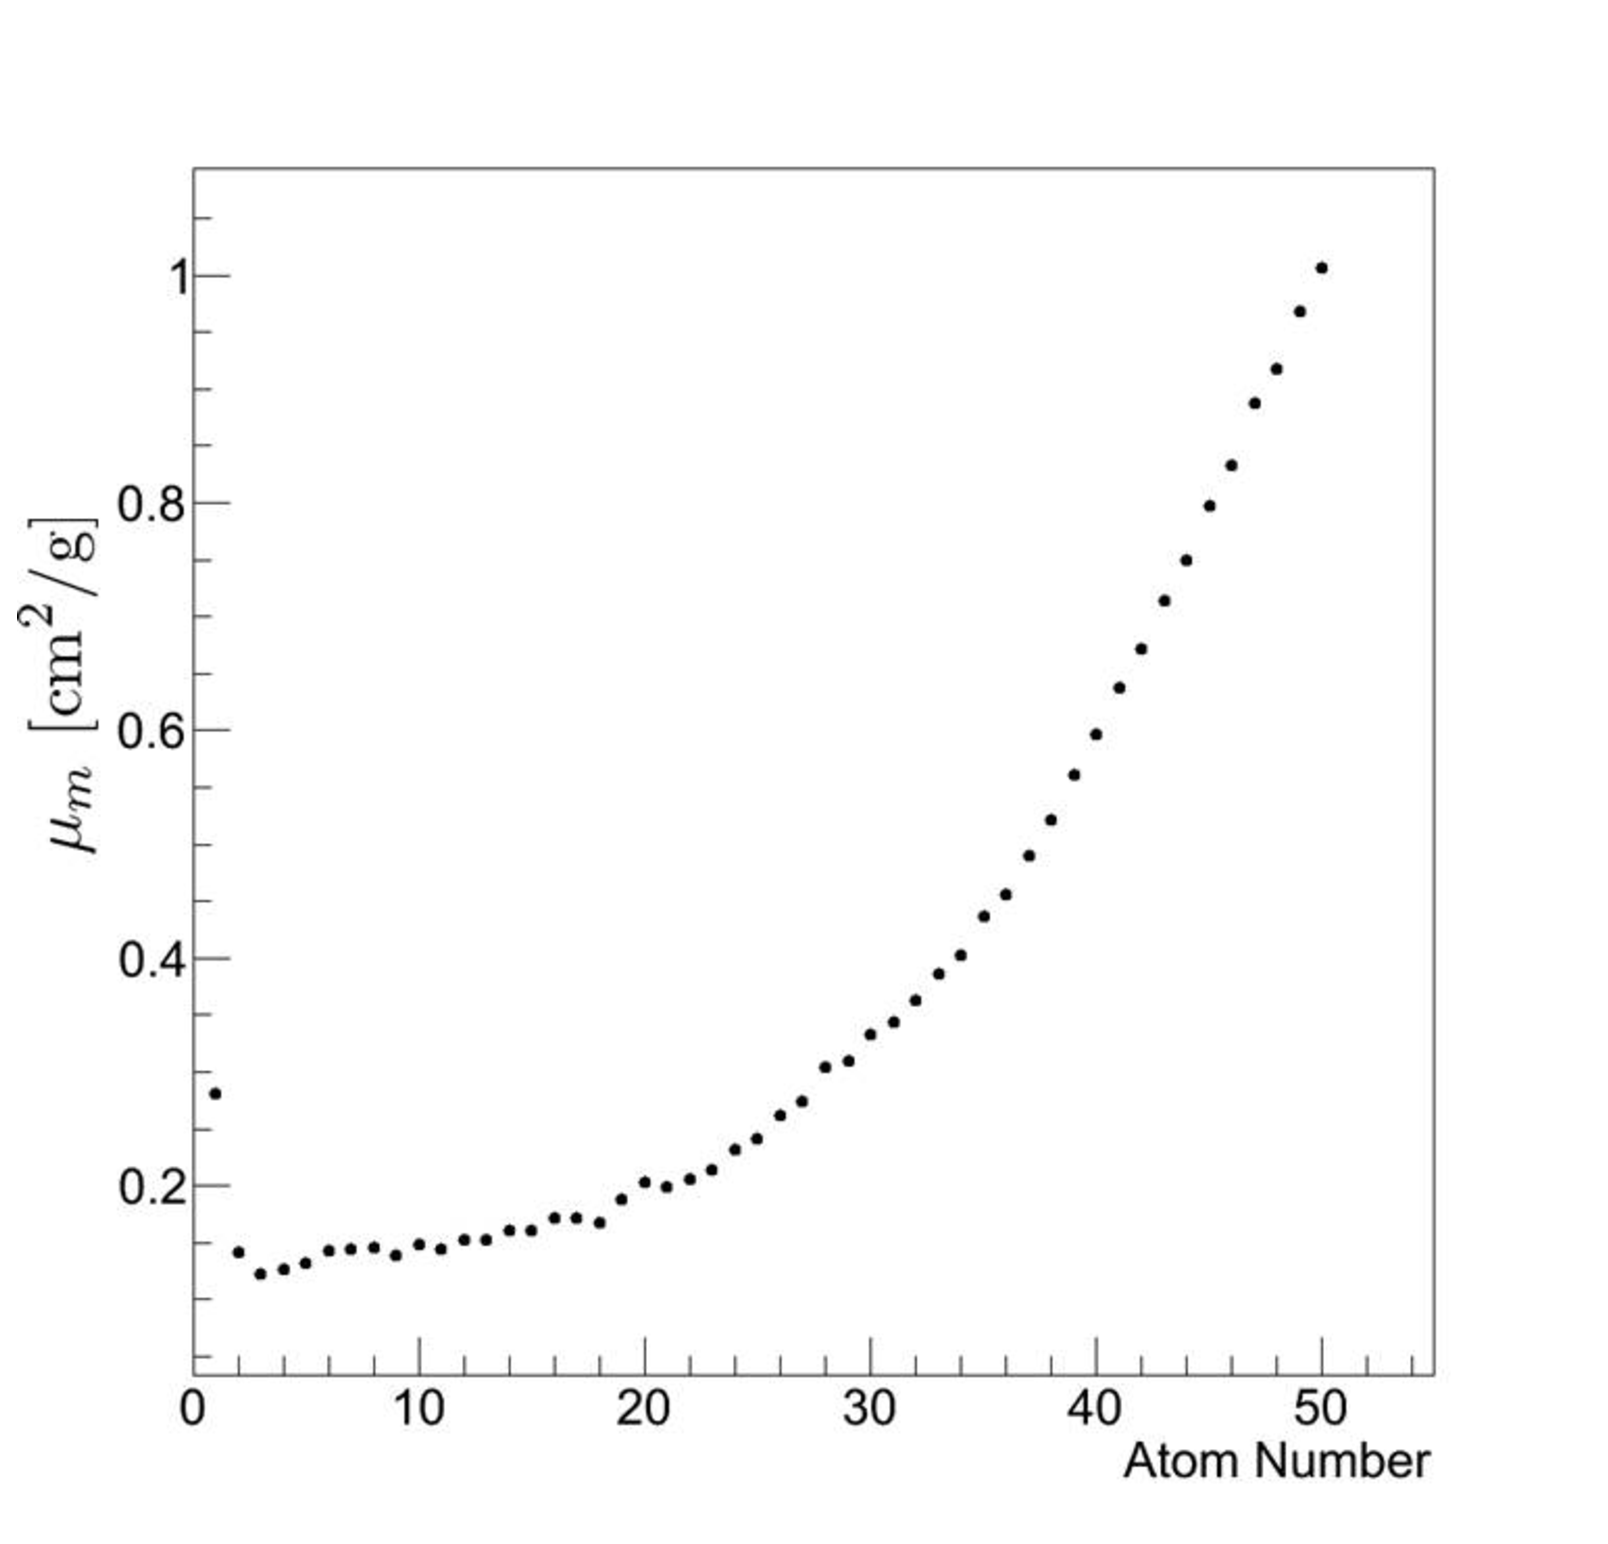
\includegraphics[width=7cm]{image/other/mass_atten.eps}
  \end{center}
 \end{minipage}
 \begin{minipage}{0.3\hsize}
  \begin{center}
   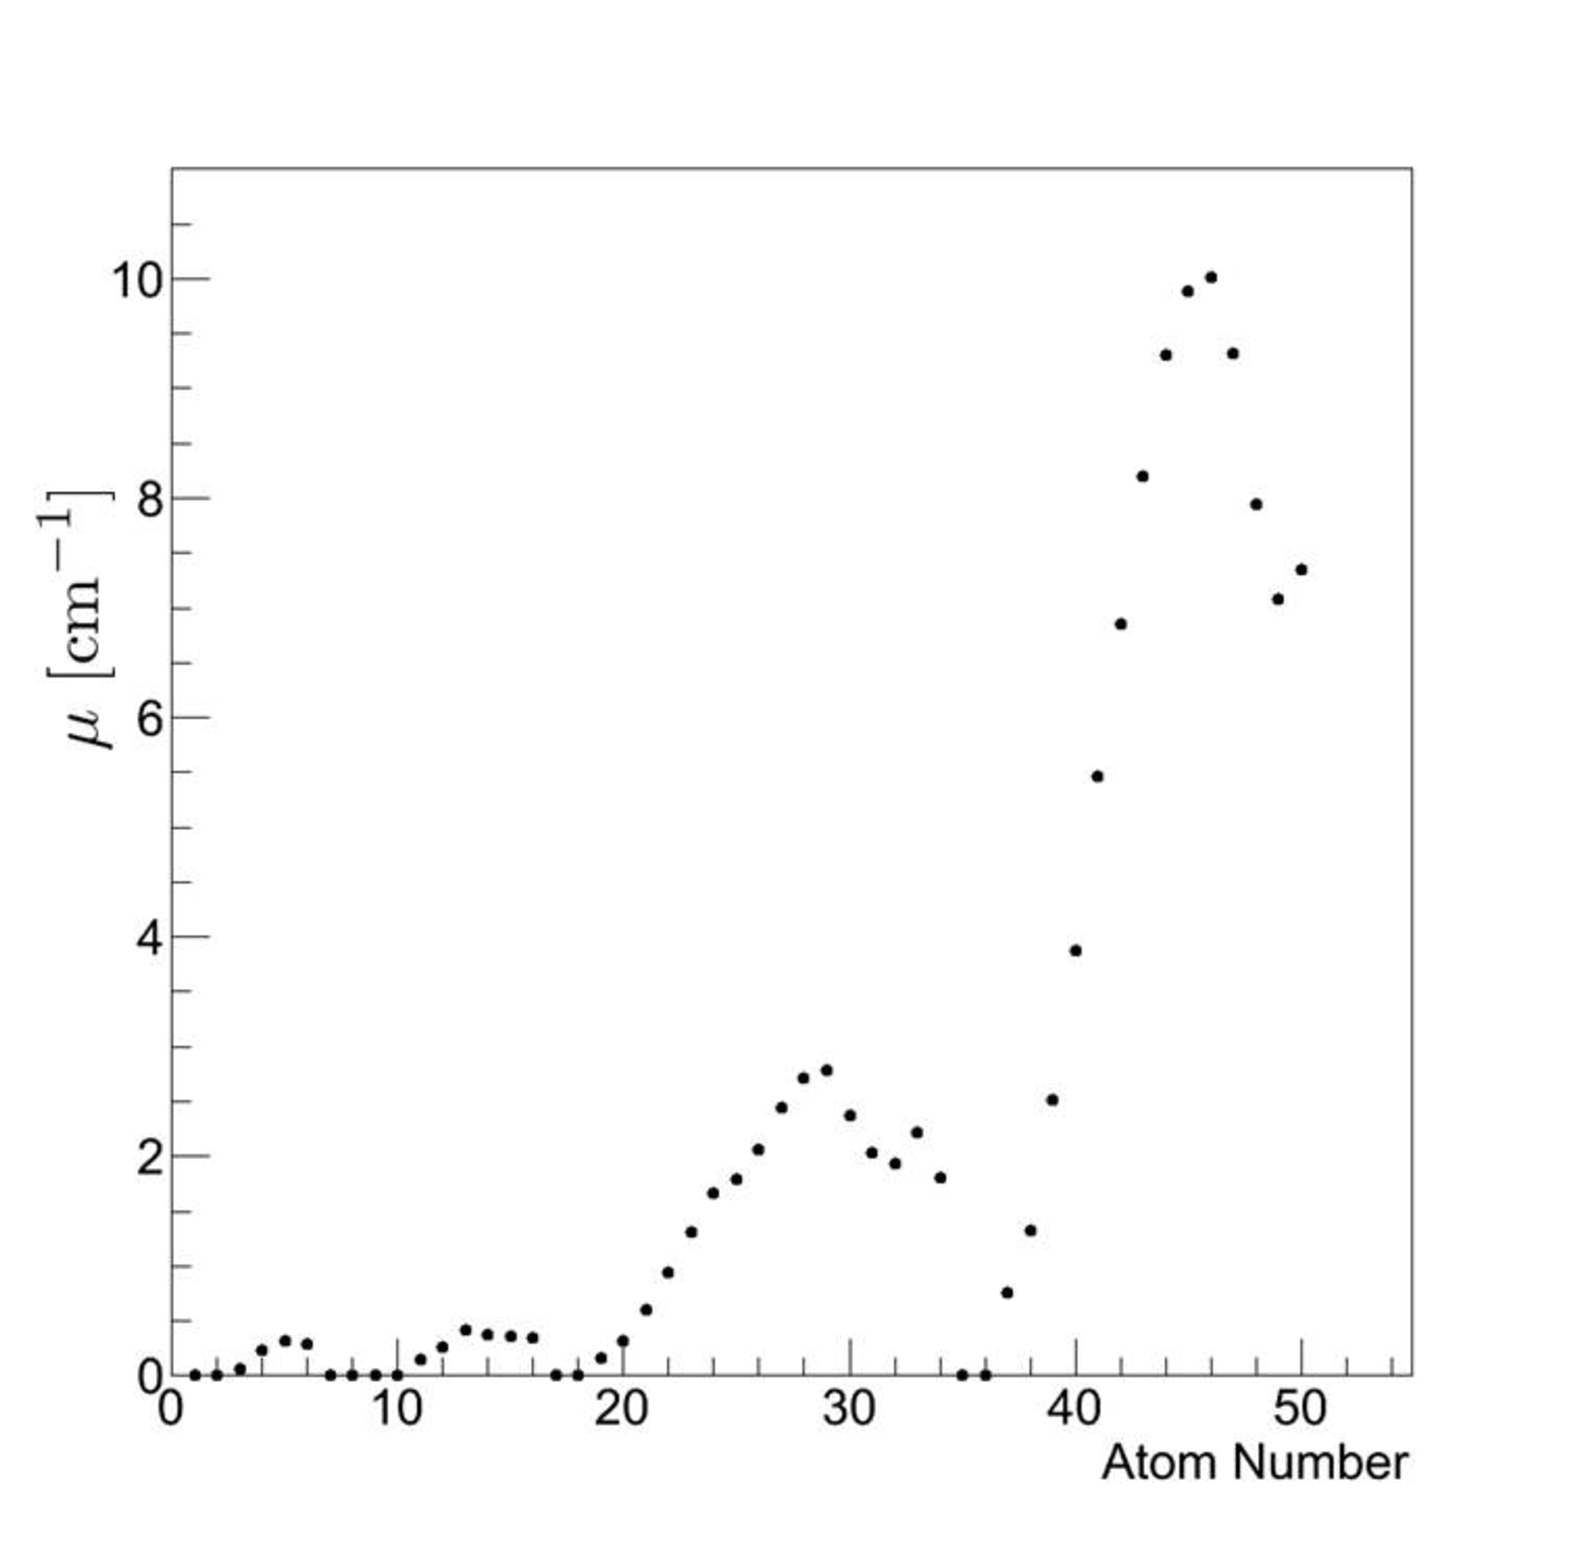
\includegraphics[width=7cm]{image/other/linear_atten.eps}
  \end{center}
 \end{minipage}
 \begin{center}
  \vspace{-1zh}
  \caption{質量減弱係数の原子番号依存性と線源弱係数の原子番号依存性(@122keV)\newline 質量減弱係数はエネルギーが一定であれば物質によって異なる値を取るが,線源弱係数は物質が異なっても同一になる場合がある}
  \label{fig:atten}
  \end{center}
\end{figure}


\subsection{ビームハードニングアーチファクト}
人体中の元素は低原子の組織が中心であるが骨の原子番号は他の組織に比べて高いため,光電効果による減弱が支配的となり,低エネルギーのX線光子が多く吸収されることになる。すなわち,X線のエネルギー分布が高エネルギー側にシフトし,その結果,実効エネルギー\footnote{平均エネルギーの意味合いとして,しばしば実効エネルギーと表現される}が高くなり線質が変化する(\Fref{fig:beam_hard})。骨の厚さは投影方向ごとに異なり、異なった線質で観測された投影データは整合性はないのでアーチファクトが生じる。人間の体はほぼ水等価物質で構成されているが,原子番号の高い骨に囲まれた部分ではアーチファクトが生じやすく、\Fref{fig:BH_artifact}に示すように骨と骨の間が黒く見えるアーチファクトが発生し、画像診断に影響を及ぼすことがある。

\if0
高原子番号の物質周辺では実効エネルギーが高くなったX線からその部位の線源弱係数$\mu$が算出されることによりCT値が低くなり,これがアーチファクトとして現れる。
\fi

\begin{figure}[H]
 \begin{minipage}{1\hsize}
  \begin{center}
   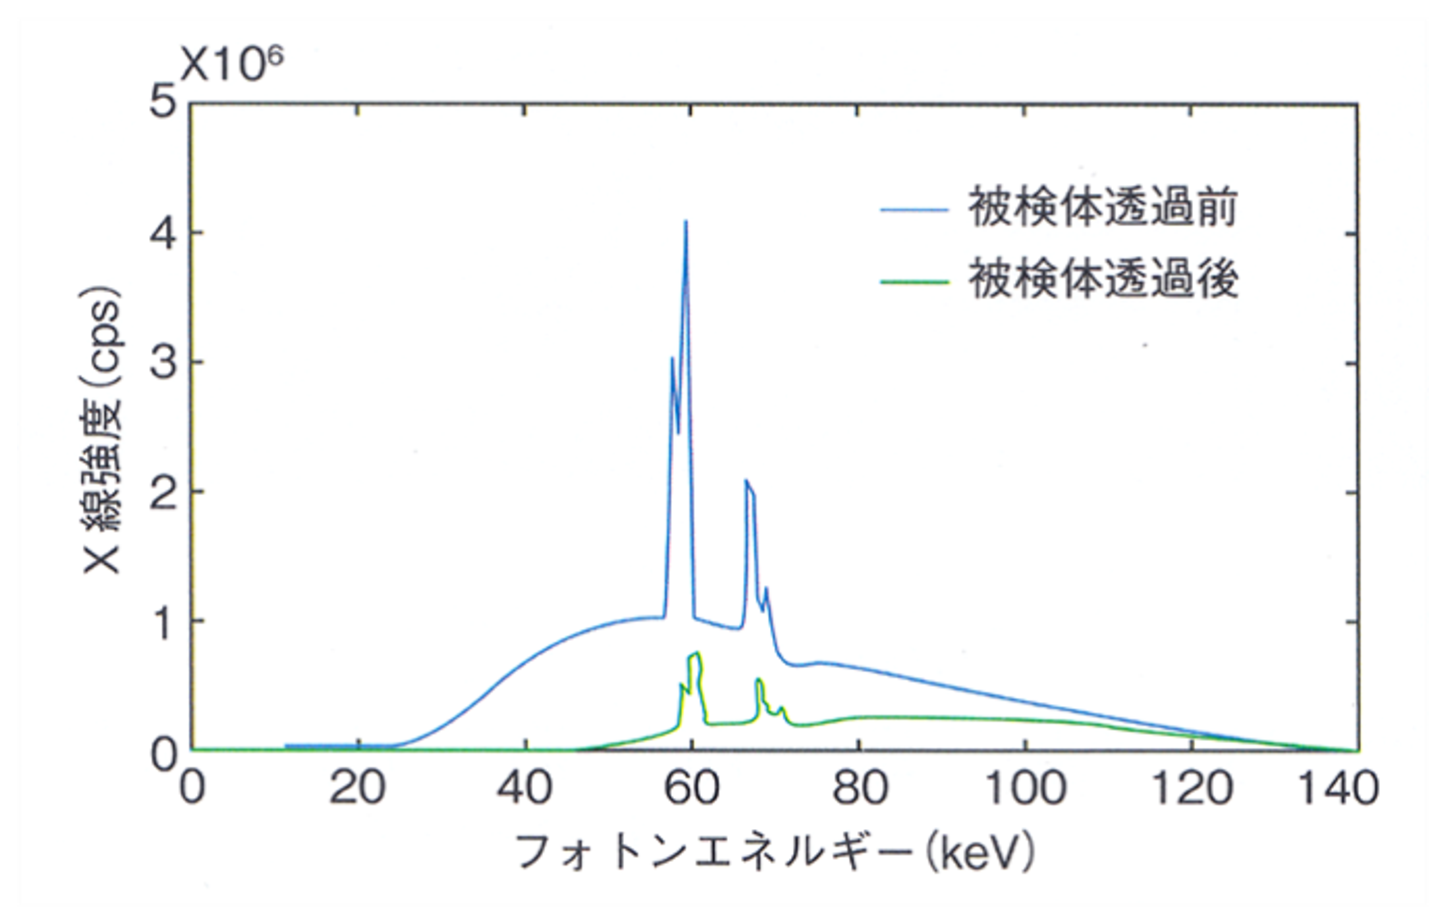
\includegraphics[width=10cm]{image/other/beam_hard.eps}
  \end{center}
  \vspace{-0.9cm}\hspace{8cm}
  
 \end{minipage}
 \begin{center}
  \vspace{-1zh}
  \caption{ビームハードニング効果\cite{spectralCT}}
  \label{fig:beam_hard}
  \end{center}
\end{figure}

\begin{figure}[H]
 \begin{minipage}{0.5\hsize}
  \begin{center}
   \includegraphics[bb=0.000000 0.000000 116.150398 147.827780,width=0.6\hsize]{image2/chapter5/BH1.png} 
  \end{center}
  \vspace{0cm}
  \caption*{頭部CT}
 \end{minipage}
 \begin{minipage}{0.5\hsize}
  \begin{center}
 \includegraphics[bb=0.000000 0.000000 153.587303 149.267661,width=0.6\hsize]{image2/chapter5/BH2.png} 
  \end{center}
  \vspace{0cm}
  \caption*{肩のCT}
 \end{minipage}
 \begin{center}
  \caption{ビームハードニングアーチファクトの例(骨と骨の内側が黒く見える)}
  \label{fig:BH_artifact}
  \end{center}
\end{figure}






\section{次世代X線CT}
上述したように通常のエネルギー積分型のCTでは,様々なエネルギーからなる混合エネルギーのX線を物質に照射し,その線源弱係数を求めCT値を画像化している。この混合したX線光子のエネルギーを分離するのは困難であり,画像化に用いられるX線エネルギーから得られる画像は1種類であるため,画像診断に用いられるパラメータはこのCT値のみとなる。その結果\ref{sec:problem}で述べたような問題が生じる。\\
\ \ そこで近年,複数のフォトンエネルギーレベルのデータを収集して画像化を行うCTが臨床応用されはじめている。このようなCTでは,画像診断に用いられるパラメータとして,複数のフォトンエネルギーレベルにおけるCT値を得ることが,通常のCTの問題点が解決される他,得られる情報が非常に多様であり通常のCTではできないイメージングが可能となる。このようなCTを次世代CTと本稿では呼ぶことにする。次世代
CTには低・高2種類の混合エネルギーのX線を照射するデュアルエナジーCTと1種類の混合エネルギーのX線を照射しパルスモード(フォトンカウンティングモード)読み出しを行うことでエネルギー帯域ごとにCT画像を取得するフォトンカウンティングCTがある。

\subsection{デュアルエナジーCT\label{sec:dual}}
デュアルエナジーCTではまず低・高2種類の混合エネルギーのX線を照射しそれぞれ別々に画像再構成する。その後,各々の画像に対して処理を施すことにより,単色X線透過画像を作成できたりと様々な画像化が可能となる。現在,実用化されているデュアルエナジーCTは以下の4方式に大別される\cite{GE}\cite{siemens}\cite{philips}。

\begin{enumerate}
\renewcommand{\labelenumi}{(\arabic{enumi})}
\item 2回転方式\\CT装置自体は通常のCTと変化しないが,1つのX線管を用い,1回転ごとに管電圧(1回転目:80kVp,2回転目:140kVp)を切り替えて撮影する方式
\begin{figure}[H]
 \begin{center}
 \includegraphics[bb=0.000000 0.000000 658.000000 447.000000,width=0.6\hsize]{image2/chapter5/dual1.png} 
 \end{center}
 \caption{2回転方式のデュアルエナジーCT}
 \label{fig:dual1}
\end{figure}

2回転方式は得られる2種類のデータの撮影時間差(時相差)が大きく,撮影時の呼吸運動や体動などの影響を受けやすく画像データ上での位置のズレなどが起こりうる。


\item 2管球方式\\設置角度の異なる2つのX線管を用い,異なる管電圧(80kVpと140kVp)で同時に撮影する方式


\begin{figure}[H]
 \begin{center}
 \includegraphics[bb=0.000000 0.000000 656.000000 234.000000,width=0.6\hsize]{image2/chapter5/dual2.png} 
 \end{center}
 \caption{2管球方式のデュアルエナジーCT}
 \label{fig:dual2}
\end{figure}
2管球方式は時相差は2回転方式に比べ短くなっているが,依然大きい(70msec)。また2つのX線管は90$^{\circ}$離れており,各検出が収集した投影データもこの管球角差$90^{\circ}$の差が反映されるため,2種類のエネルギーデータが1:1に対応しない。これらの理由によりこの2方式では投影データではなく画像データに基づいてデュアルエナジーCTの画像化を行うため,時相差によるミスレジストレーション\footnote{重ね合わせる用紙や画像などの位置ずれを示す}が生じやすい。

\item 1管球高速kVpスイッチング方式\\1つのX線管を用い,ビュー毎に高速で管電圧を切り替えて(80kVpと140kVp)撮影する方式


\begin{figure}[H]
 \begin{center}
 \includegraphics[bb=0.000000 0.000000 640.000000 480.000000,width=0.6\hsize]{image2/chapter5/dual3.jpg} 
 \end{center}
 \caption{1管球高速kVpスイッチング方式のデュアルエナジーCT}
 \label{fig:dual3}
\end{figure}

1管球高速kVpスイッチング方式は2管球ではなく1つのX線管球を用いて異なる2種類の管電圧を高速に切り替えて撮影を行うので時相差は0.5msec以下であり,管球差は当然ない。従って,時間的及び空間的にほぼ完全に一致した投影データに基づいて解析を行うことができる。現在臨床応用されているのは3つのうちこの方式のみである。投影データから解析を行うことで単色X線透過画像が取得でき既に多数の臨床応用例がある\cite{spectralCT}。

\item 2層式検出器によるデュアルエナジーCT

\begin{figure}[H]
 \begin{center}
 \includegraphics[bb=0.000000 0.000000 470.361117 368.609528,width=0.6\hsize]{image2/chapter5/dual4.png} 
 \end{center}
\caption{2層式検出器方式\cite{philips}}
 \label{fig:two_layer}
\end{figure}

\if0
\begin{figure}[H]
 \begin{center}
 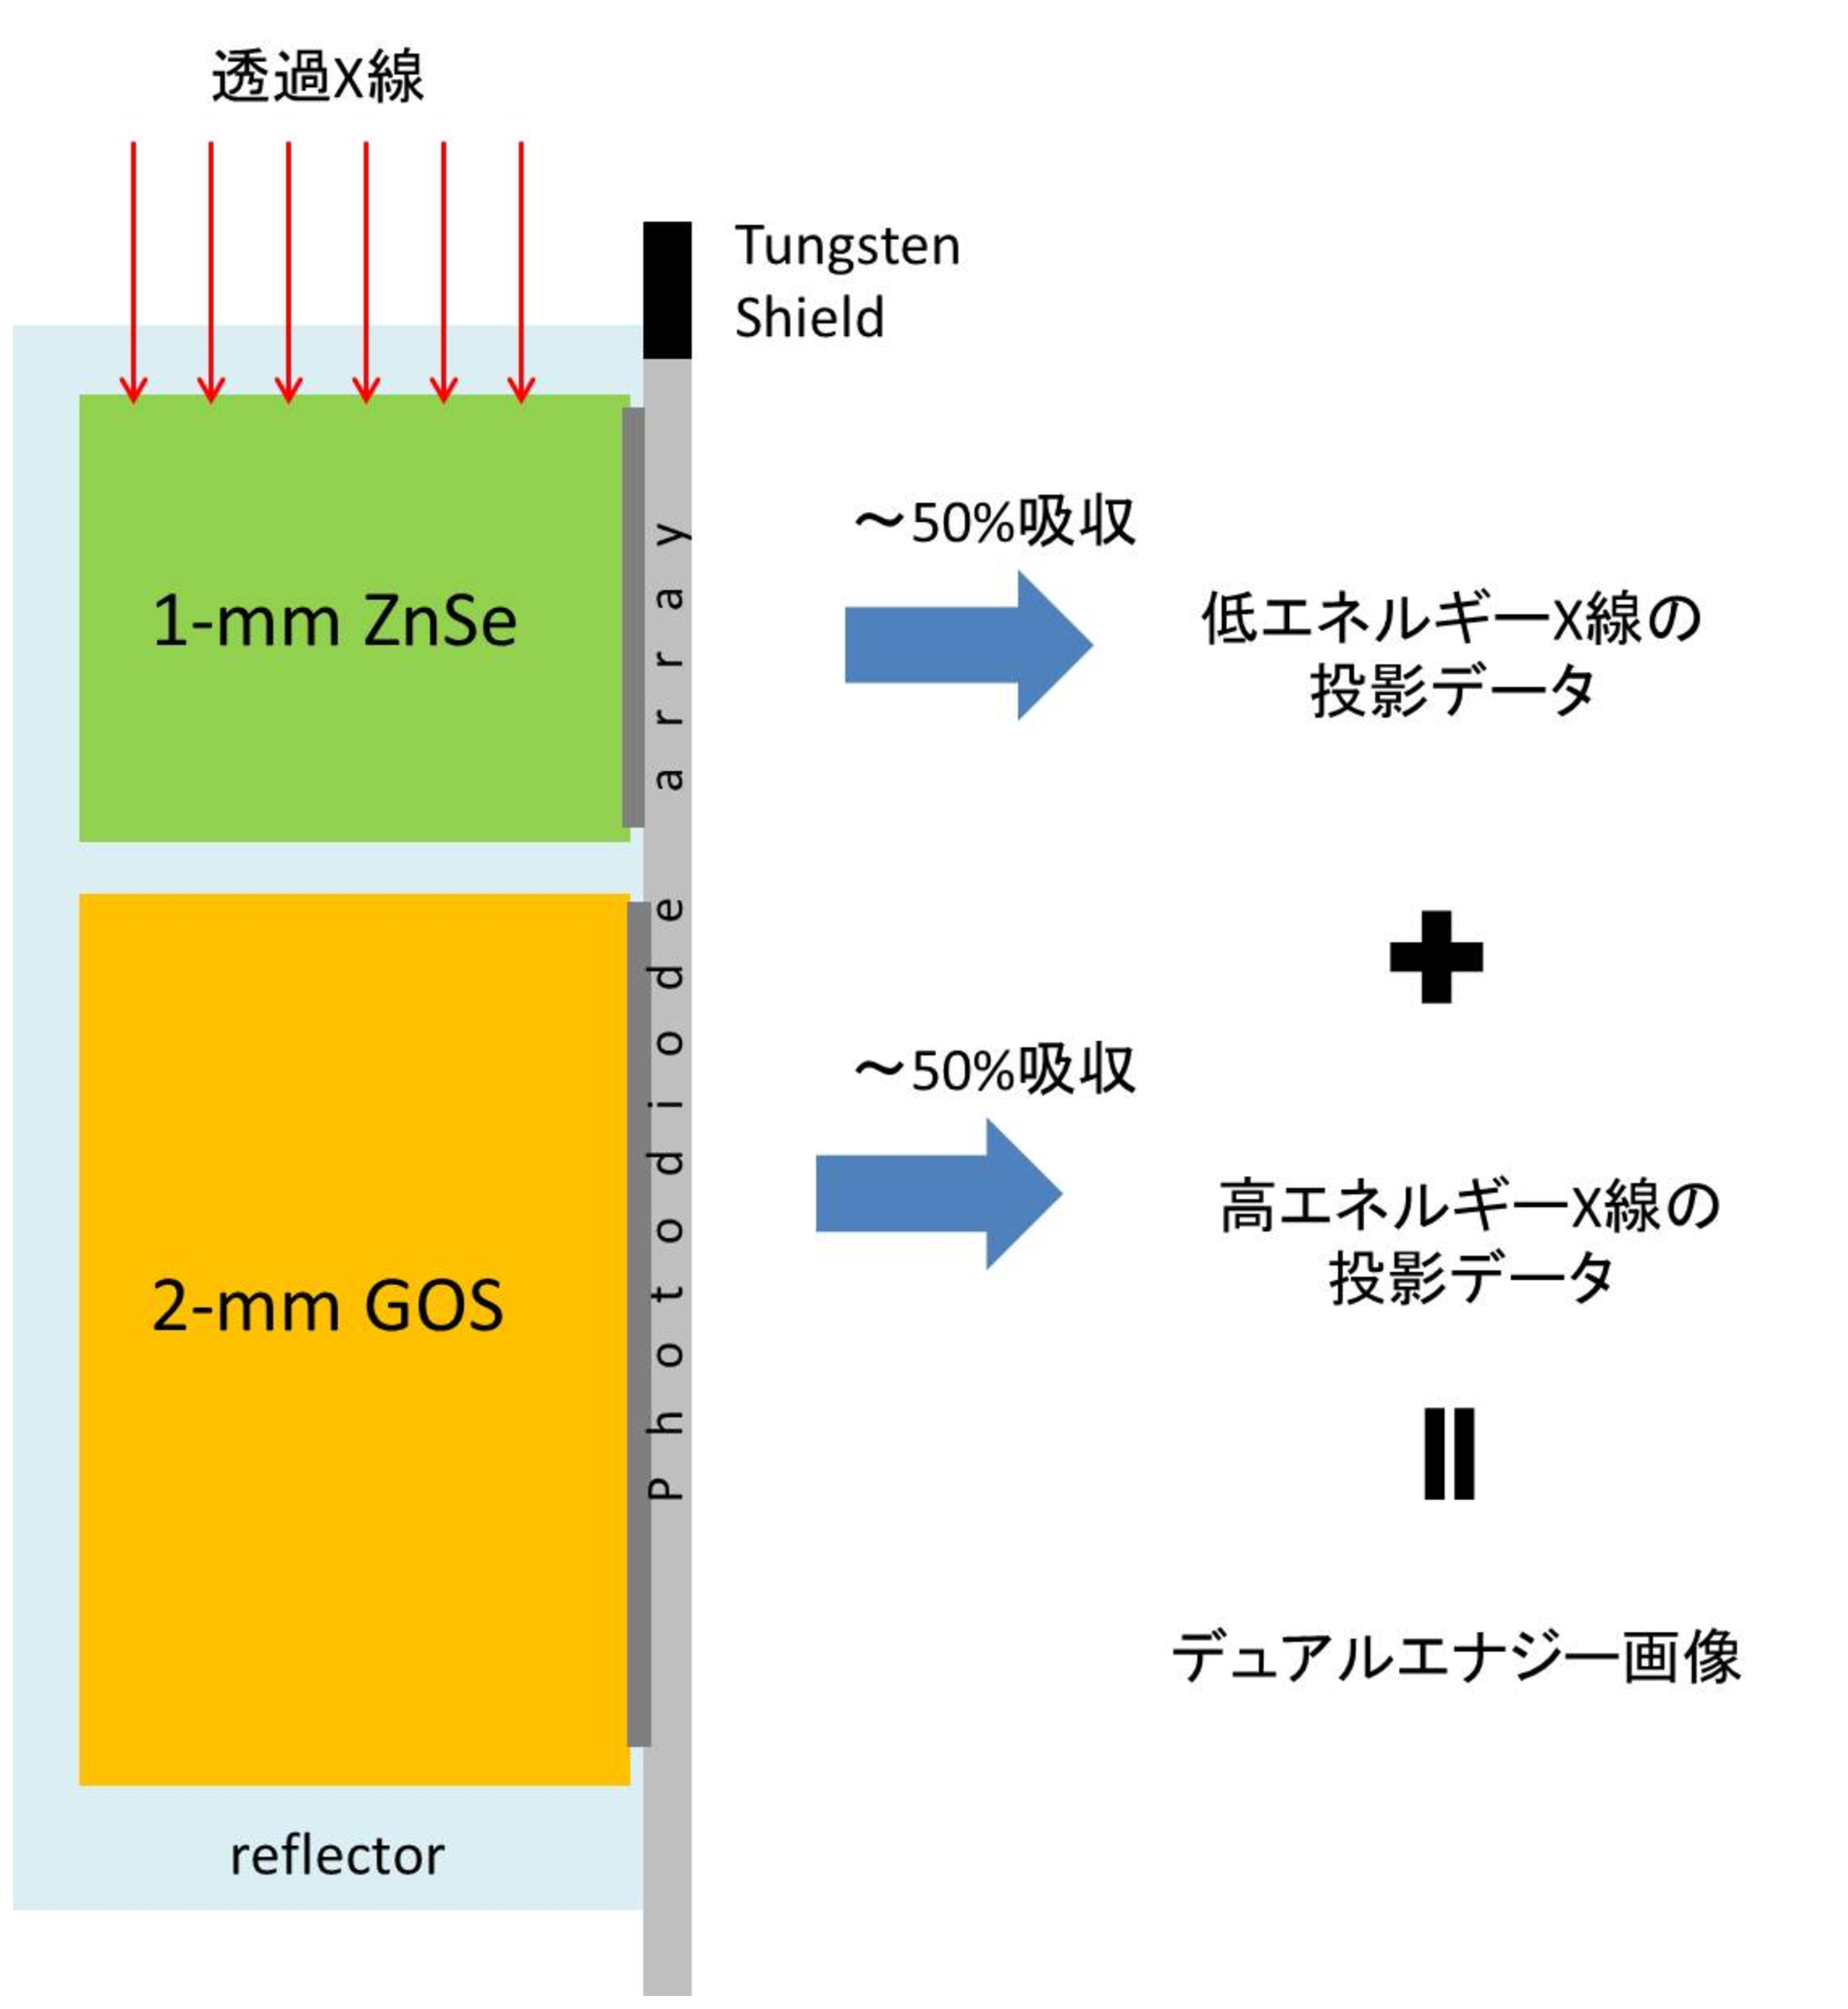
\includegraphics[width=7cm]{image/other/two_layer.eps}
 \end{center}
 \caption{2層式検出器方式\cite{philips}}
 \label{fig:two_layer}
\end{figure}
\fi

また別のアプローチのデュアルエナジーCTとして,2層式検出器方式がある(\Fref{fig:two_layer})。これは検出器は異なる材料の2層式の構造になっており,被写体を透過してきたX線はまずCsI,ZnSeなど低エネルギーにしか感度を持たない上層のシンチレータで低エネルギーのX線光子のみが吸収され,この低エネルギー成分から投影データをまず1つ作成することができる。その後,高エネルギー成分が下層の($\rm Gd_2O_2S(GOS)$)によって吸収され,高エネルギー成分のデータからもう1つ投影データを作成することが出来る。こうして低エネルギー,高エネルギーに対する2種類の投影データを作成することができ,投影データに基づいたエネルギー解析により,デュアルエナジーCTの画像化が行われる。この手法においては空間的,時間的なズレは全くなくなるが,高・低エネルギーX線を完全に二層の検出器で分けることはできず,重複領域が大きい。さらにX線上層の検出器を透過する際,大量の散乱線が生じうる,下層の検出器により得られるエネルギーデータに悪影響を及ぼす可能性があるなどの問題がある。\\\ \ 二層式の検出器は空港手荷物用のX線検査装置に利用されており実用化されている場面もある\cite{airport_1}\cite{airport_2}。

\end{enumerate}

\subsection{フォトンカウンティングCT\label{sec:CT_photon}}
フォトンカウンティングCTは1つのX線管により1種類の管電圧で撮影するため,通常のCTと同様に用いるのは1種類の混合エネルギーX線のみである。この1種類の混合エネルギーX線に対して,検出器においてX線を構成する各フォトンのエネルギーが計測され,エネルギー帯域ごとに分けてカウントし,エネルギー帯域別にCT画像を出力するのがフォトンカウンティングCTである。デュアルエナジーCTでは2種類のX線を照射するので患者の被曝量は通常のCTよりも多くなるが,フォトンカウンティングCTでは1種類のエネルギーのX線のみ用いればよいため被曝量は増えず,管電圧スイッチングに伴う時相差はまったく生じない。また,フォトンカウンティングCTは各々のフォトンをエネルギー帯域別にカウントでき,マルチエナジー画像の再構成が容易である。\\
\ \ フォトンカウンティングCTを実現するためには,パルス読み出しを行う必要がある。そのためには,光検出器が高い増幅率を持ち,S/Nが高い必要がある。さらに従来のCTの画質とスピードを実現するためには10$^6$counts/sec/mm$^2$という高計数に耐えなければならない。従って,シンチレータ側には従来のCTの要求に加えてパイルアップを防ぐために減衰時間が短い必要がある。\\ 
\ \ 現在のX線CTに用いられているGOSは減衰時間が$\sim$3$\mu$sと非常に長く,高計数に対応することはできない。また増幅機能を持たないPDを用いることでノイズ耐性は低く,そもそもパルス読み出し自体が困難である。さらにPDの数が膨大なためデータ処理の面からもパルス読み出しは困難である。従ってシンチレーション検出からフォトンカウンティングCTへのアプローチではなく,エネルギー分解能が高い半導体を用いたフォトンカウンティングCTが現在のトレンドとなっている。現在最も広く研究されてい応用されているフォトンカウンティング検出器はテルル化カドミウム(CdTe)とテルル化亜鉛カドミウム(CdZnTe:CZT)素材の半導体検出器である\cite{ogawa}\cite{ogawa_id}\cite{kowase}\cite{Adam}\cite{Jan}。エネルギー分解能は$4.4\%$(FWHM@122keV)を実現している\cite{ogawa}。しかし,\ref{sec:CdTe}で述べたが,CdTeは電荷収集時間が遅く,さらに増幅機能を持たないため,長い時定数でのチャージセンシティブアンプの使用が不可欠であり,高計数には対応しないという問題がある。\\\ 以下にフォトンカウンティングCTの通常のCTと比べた場合の利点に関して述べる。

\subsubsection*{ビームハードニングの低減}
スペクトラルCTではX線の投影データをエネルギー帯域別に取得するため,ビームハードニングは起こらない。エネルギー帯域ごとに取得した画像に対して高エネルギーの画像の重みを多くして画像を合成することにより,ビームハードニングのアーチファクトを低減することができる\cite{kowase}。また,実際の診断においてスペクトラルCTによるアーチファクトの低減例\cite{spectralCT}を\Fref{fig:artifact_1}と\Fref{fig:artifact_2}に示す。

\begin{figure}[H]
 \begin{minipage}{0.52\hsize}
  \begin{center}
   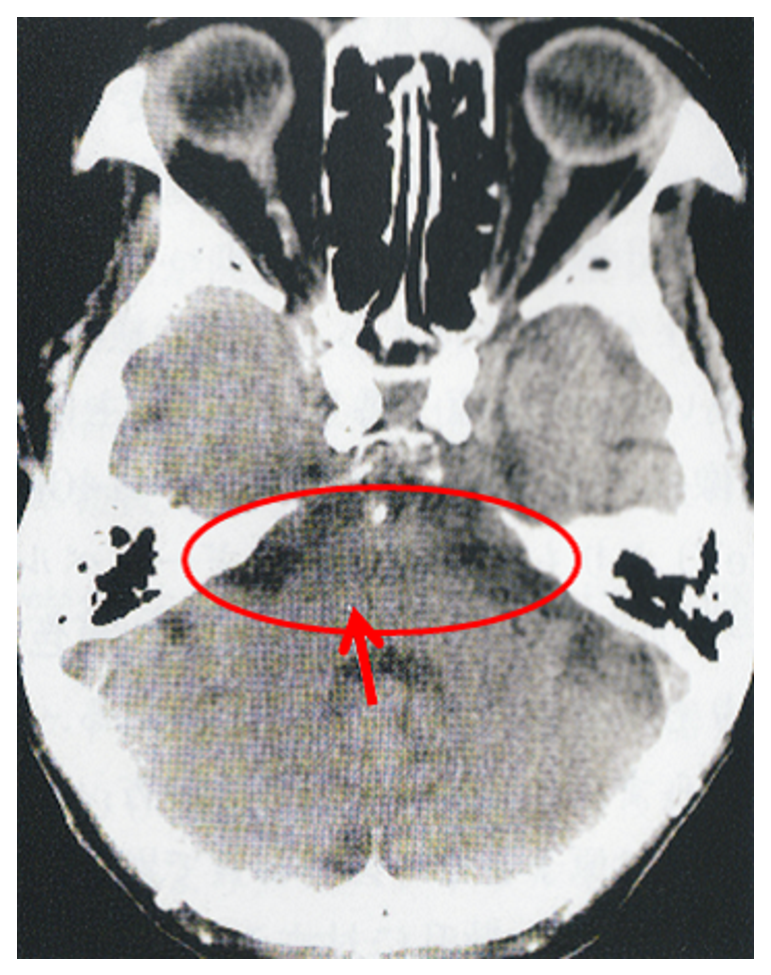
\includegraphics[width=5cm]{image/other/artifact_1.eps}
  \end{center}
  \vspace{-0.5cm}\hspace{1cm}
   (a)エネルギー積分型CT画像(140kVp)
 \end{minipage}
   \begin{minipage}{0.5\hsize}
  \begin{center}
   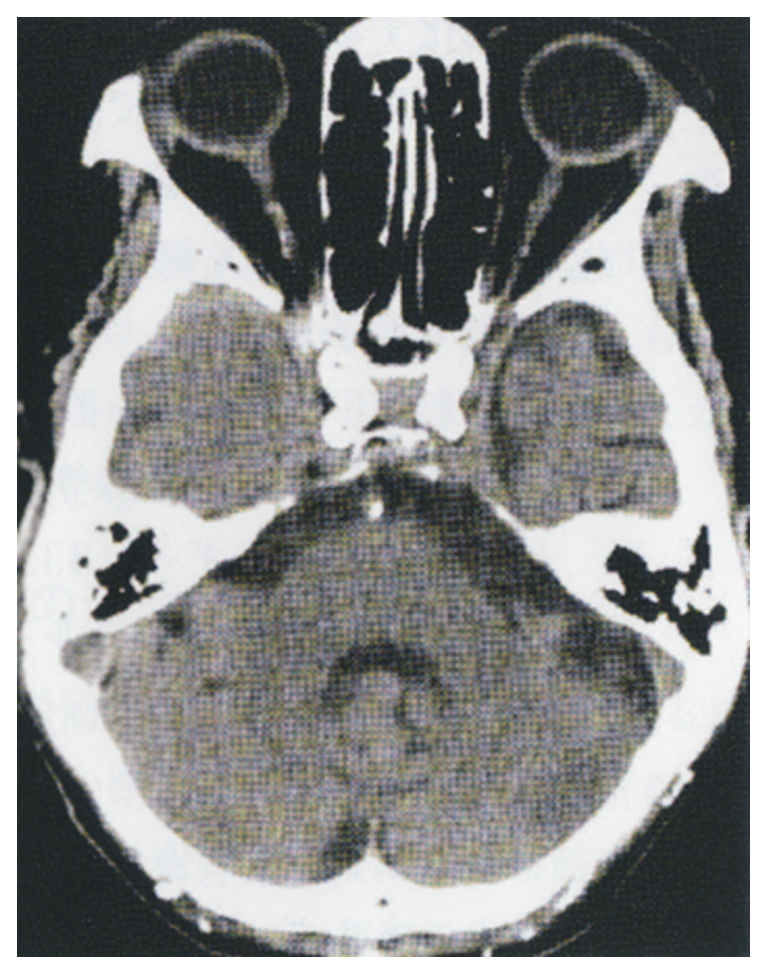
\includegraphics[width=5cm]{image/other/artifact_1_after.eps}
  \end{center}
  \vspace{-0.5cm}\hspace{2cm}
   (b)スペクトラルCT(70keV)
 \end{minipage}
 \begin{center}
  \vspace{-1zh}
  \caption{後頭蓋窩アーチファクトの低減\cite{spectralCT}:(a)には赤丸部に橋を横切るような線状の低吸収域が見られる。これにより脳幹や小脳などの描画不明瞭にとなりやすく,同部の出血や梗塞などの診断には限界がある。(b)ではこのアーチファクトが低減され,脳実質の観察が容易になる。}
  \label{fig:artifact_1}
  \end{center}
\end{figure}


\begin{figure}[H]
 \begin{minipage}{0.52\hsize}
  \begin{center}
   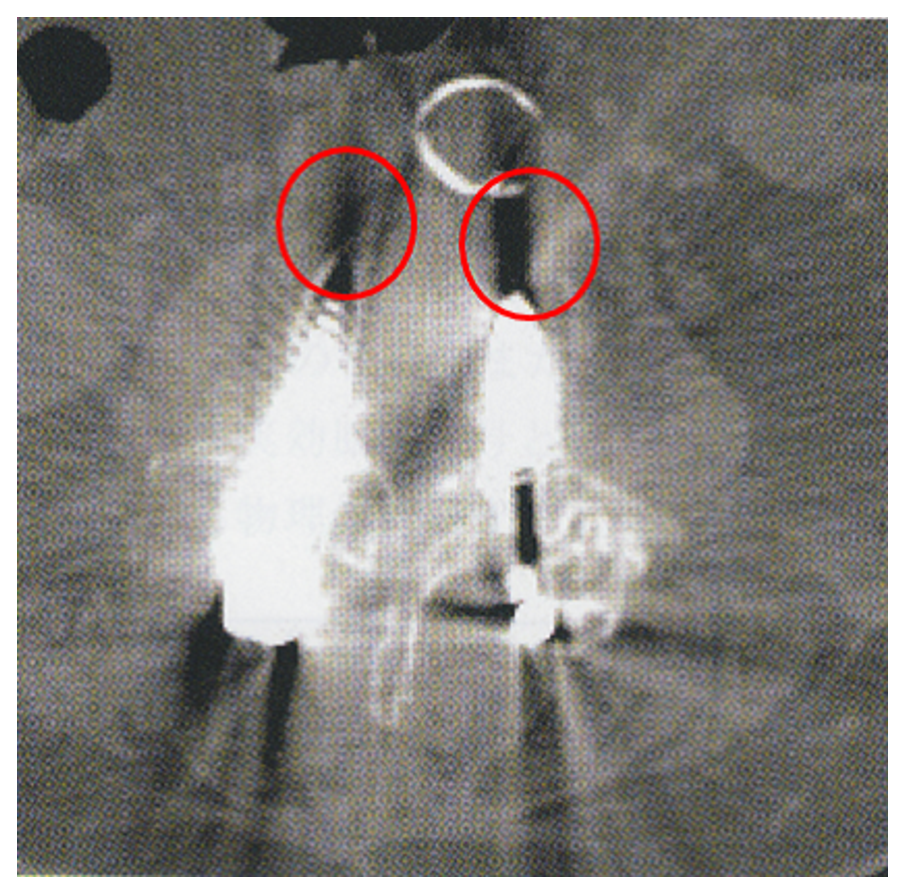
\includegraphics[width=5cm]{image/other/artifact_2.eps}
  \end{center}
  \vspace{-0.5cm}\hspace{1cm}
   (a)エネルギー積分型CT画像(140kVp)
 \end{minipage}
   \begin{minipage}{0.5\hsize}
  \begin{center}
   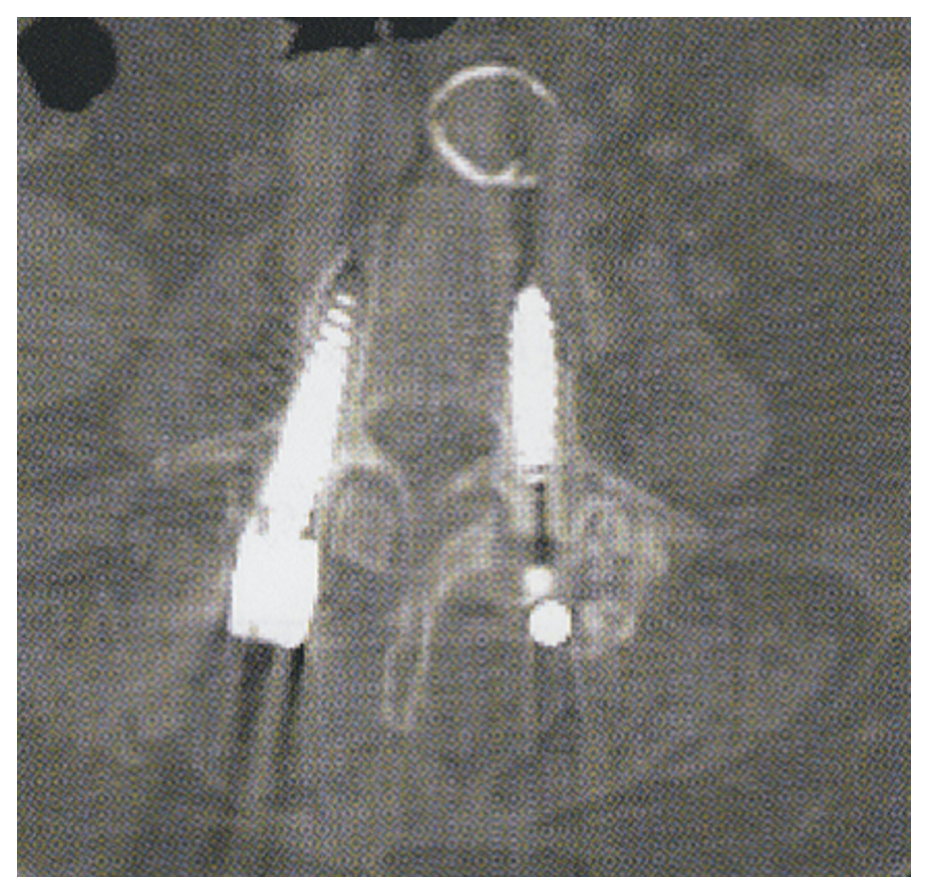
\includegraphics[width=5cm]{image/other/artifact_2_after.eps}
  \end{center}
  \vspace{-0.5cm}\hspace{2cm}
   (b)スペクトラルCT(70keV)
 \end{minipage}
 \begin{center}
  \vspace{-1zh}
  \caption{金属アーチファクトの低減\cite{spectralCT}:金属スクリューを用いた腰椎後方固定術後症例で(a)では金属アーチファクトのためスクリュー自体およびその周辺組織の評価が困難となっているが,(b)では金蔵アーチファクトが著明に低原子,周辺組織の評価が容易になる。}
  \label{fig:artifact_2}
  \end{center}
\end{figure}
\subsubsection*{媒質の同定}
先述のように従来のエネルギー積分型のCTでは,線源弱係数は物質が異なっても密度によっては同一になる場合があり,パラメータは一つのCT値のみであったため正確な物質の弁別をすることができなかった。しかし,スペクトラルCTではいくつかのエネルギー帯においてCT値を取得することができるため,パラメータが複数になることで正確な材質の弁別が可能となる。例えば,ある領域に対して低エネルギーと高エネルギーによる線源弱係数を求めたとする。その比($\mu(E_{\rm Low})/\mu(E_{\rm High})$)の原子番号依存性は既知であり,対象組織の密度,厚さに依存せず原子番号のみに依存する。(\Fref{fig:rate}参照)。すなわち,低エネルギー領域と高エネルギー領域の線源弱係数の比を求めることによって,検査対象の組織の原子番号を求めることができる\cite{material_id}。\\
\ \ また,各エネルギー帯ごとに線源弱係数を求めた後,そのエネルギー依存性を既知の候補物質の線源弱係数のエネルギー依存曲線と比較することにより媒質を同定する手法もある\cite{ogawa_id}。



\subsubsection*{軟部組織のコントラスト強調}
エネルギーごとに投影データを得て,これに対して重み付けを行うことによって,特定の媒質のコントラスト自由に変えることができる。\Fref{fig:material_atten}に示すようにX線光子のエネルギーが低いほど光電吸収が支配的になるので線源弱係数の物質間での差が高エネルギーより大きくなるので,低エネルギー画像に多く重みを付けることによりコントラストを強調することができる。特にこれは軟部組織のイメージングのように線源弱係数が低エネルギーのみでしか変化しないような場合に有効である\cite{kowase}\cite{ogawa_kaisetu}。

\begin{figure}[H]
 \begin{center}
 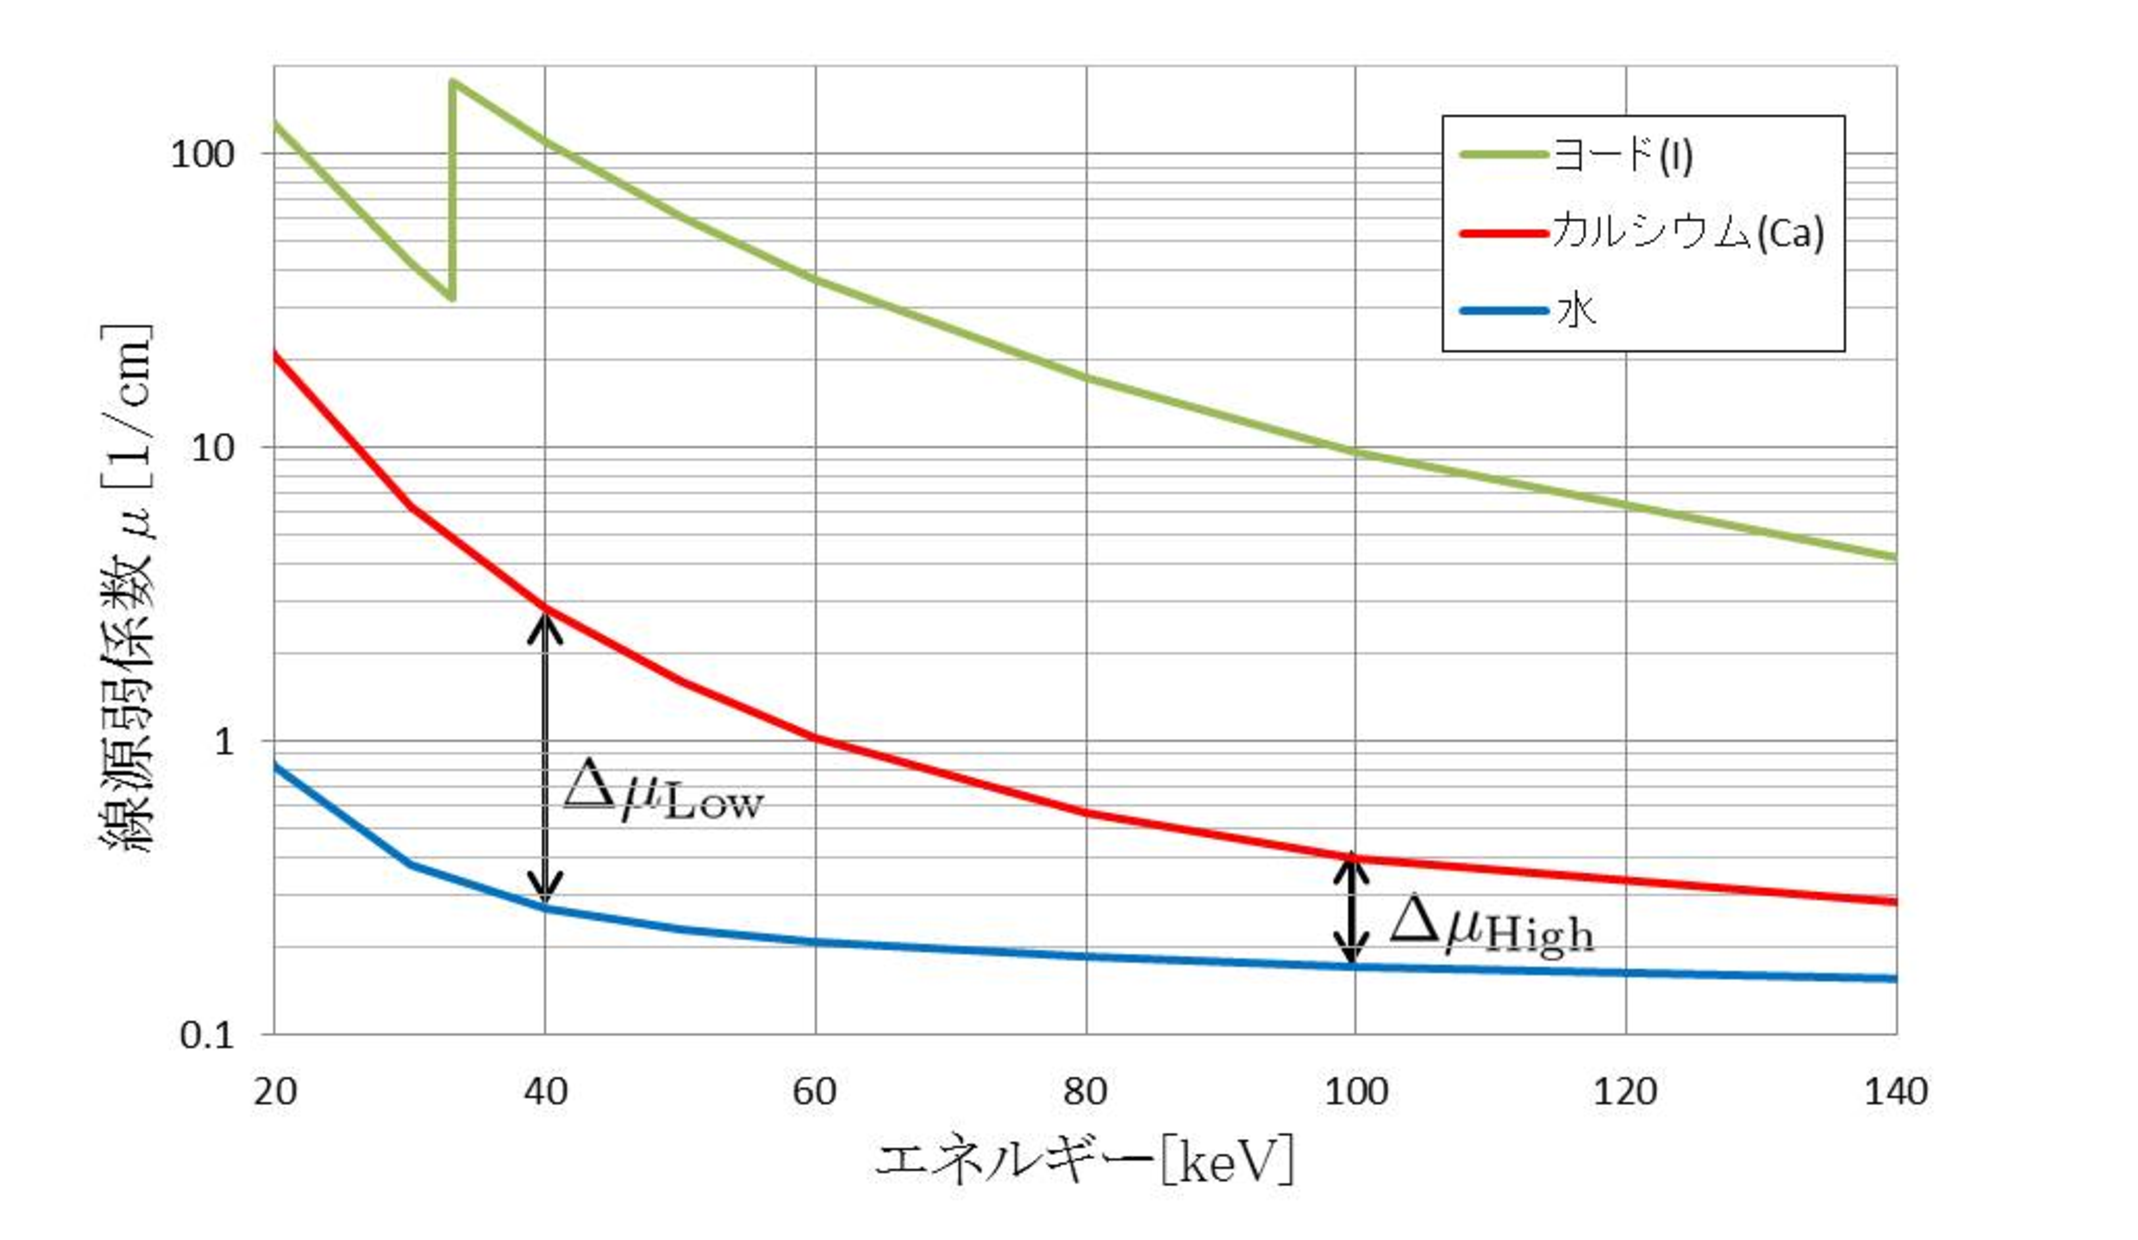
\includegraphics[width=10cm]{image/other/material_atten.eps}
 \end{center}
  \vspace{-0.7cm}
 \caption{ヨード,カルシウム,水の線源弱係数(NISTより作成)\newline $\Delta\mu_{\rm Low}$が$\Delta\mu_{\rm High}$より大きいため低エネルギーにおける画像の方がコントラストが強調される}
 \label{fig:material_atten}
\end{figure}


\subsubsection*{ノイズの低減(SN比の向上)\label{sec:pulse_merit}}
フォトンカウンティング方式にすることによって電子的なノイズを低減することができる。データの計測時には,アナログ系の電子的ノイズが混入し,その計測値に誤りを発生させるこになる。\Fref{fig:noise_affect}(a)は70kVのX線管から発生したX線の理想的なエネルギースペクトルと,ある量の水を透過した後のエネルギースペクトルを模式的に示したものである。実際の計測においては計測対象の透過X線は,X線発生時における統計的な変動,高圧や管電流の揺らぎの影響を受け,さらに計測時に混入する電子的ノイズによって\Fref{fig:noise_affect}(b)のようなスペクトルを計測することになる。この時,従来のエネルギー積分型の計測を行うとそのノイズ成分は加算され影響を与えることになるが,フォトンカウンティング型ではエネルギー帯域ごとX線光子が個数としてカウントされるので,ノイズの影響は受けにくくなる。このような電子的ノイズが大きく影響を与えるのは,計数時のX線の強度が非常に小さくなる場合である。

\begin{figure}[H]
 \begin{center}
 \includegraphics[width=12cm]{image/other/noise_affect.eps}
 \end{center}
 \caption{エネルギー積分型CTとスペクトラルCTにおけるノイズの影響の比較\cite{ogawa_kaisetu}}
 \label{fig:noise_affect}
\end{figure}

\subsubsection*{K吸収端イメージング}
従来のエネルギー積分型の方式では実現できないイメージングがK吸収端イメージングである。人体を構成する元素の大部分は原子番号が非常に小さいため,K吸収端は低エネルギーレベルに存在するため,そのK吸収端を捉えることは不可能であるが,造影剤として用いるガドリニウム(Gd)やヨード(I)のK吸収端はそれぞれ50.2keV,33.2keVであり,K吸収端の前後でデータの計測を行うことで造影剤の分布を特異的に示すことができる。例えばGdの場合bin0:40-49keV,bin1:50-59keVとしそれぞれのbinでCT画像を再構成した後,bin1のCT画像からbin0のCT画像を引き算することにより,造影剤を含んだ血管や組織などの明瞭な画像下が可能となる。

\begin{figure}[H]
 \begin{center}
 \includegraphics[width=12cm]{image/other/k-edge.eps}
 \end{center}
 \vspace{-0.7cm}
 \caption{K吸収端イメージングの原理(減弱曲線はNISTより作成)}
 \label{fig:k-edge}
\end{figure}









	% 本文4
\fi

\chapter{低被ばく化の実証}


%素子について
本章では従来のCTに用いられるPDと次世代光センサーであるAPDとMPPCを用いて画像の比較を行う。用いた検出器の外観を\Fref{fig:soshi}に、基本特性を\Tref{soshi_tokusei}示す。

\begin{figure}[H]
 \begin{minipage}{0.5\hsize}
  \begin{center}
   \includegraphics[bb=0.000000 0.000000 300.000000 367.000000,width=0.6\hsize]{image2/chapter5/PD_APD.png} 
  \end{center}
  \vspace{-0.5cm}
  \caption*{PD,APD}
 \end{minipage}
 \begin{minipage}{0.5\hsize}
  \begin{center}
 \includegraphics[bb=0.000000 0.000000 300.000000 367.000000,width=0.6\hsize]{image2/chapter5/MPPC_picutre.png} 
  \end{center}
  \vspace{-0.5cm}
  \caption*{MPPC}
 \end{minipage}
 \begin{center}
  \caption{実験に使用したPD,APD(左)とMPPC(右)}
  \label{fig:soshi}
  \end{center}
\end{figure}

\if0
\begin{figure}[H]
 \begin{center}
 \includegraphics[width=10cm]{image2/chapter5/apd_mppc.eps}
 \end{center}
 \caption{実験に使用したPD,APD(左)とMPPC(右)}
 \label{fig:Xray}
\end{figure}
\fi

% Table generated by Excel2LaTeX from sheet 'Sheet1'
\begin{table}[H]
  \centering
    \begin{tabular}{ccc}
    \toprule
          & PD,APD  & MPPC \\
    \midrule
    型番    & S8664-11 &  S12571-050C \\
    受光面   & 1mm$\times$1mm & 1mm$\times$1mm \\
    \multirow{2}[0]{*}{動作電圧VR[V] (at 25 ℃)} & 50 (M=1) & \multirow{2}[0]{*}{66.58} \\
          & 394.1 (M=50) &  \\
    \multirow{2}[0]{*}{ゲイン} & PD : 1 & \multirow{2}[0]{*}{1:25$\times$ $10^6$} \\
          & APD : 50 &  \\
    最大感度波長[nm] & 420   & 450 \\
    \bottomrule
    \end{tabular}
     \caption{実験に使用したPD,APD,MPPCの基本特性}
  \label{soshi_tokusei}
\end{table}

PDとAPDでは同一の素子を用いて、印加電圧を変えることでPDはゲイン1、APDではゲインが50とした。この時のPD,APD印加電圧は実際に逆バイアス電圧を変化させて取得した\Fref{fig:apd_gain}のゲイン特性より決定した。

\begin{figure}[H]
 \begin{center}
 \includegraphics[width=7cm]{image2/chapter5/apd_gain.eps}
 \end{center}
 \caption{APDのゲイン特性(at 25℃)※rootの画像に差し替える}
 \label{fig:apd_gain}
\end{figure}


%読み出し回路
またMPPCにおいては従来のエネルギー積分型の読みだし方法である「電流モード」と、X線透過光子一つ一つのエネルギーを弁別する「パルスモード」での画像取得を行った。電流モードにおいてはKeithley237を用いて検出器からの電流値を一定間隔で読み出すことで投影データを取得した。パルスモードにおいてはMPPCからの信号をアンプを用いて10倍に増幅し、整形アンプ(時定数100ns)を通り、コンパレーターで閾値を設定しパルスを生成し、カウンタカードでそれをカウントした。また、パルスモードに置いては浜松フォトにクスの温度保証モジュールを用いた。実験のセットアップを\Fref{fig:CTsetup}に、電流モードとパルスモードの読み出し回路を\Fref{fig:read_circuit_current}と\Fref{fig:read_circuit_pulse}にそれぞれ示す。

\begin{figure}[H]
 \begin{center}
 \includegraphics[bb=0.000000 0.000000 625.388301 214.062304,width=0.8\hsize]{image2/chapter5/setup.png} 
 \end{center}
 \caption{実験セットアップ※アルミニウムフィルターをつける}
 \label{fig:CTsetup}
\end{figure}



\begin{figure}[H]
 \begin{center}
 \includegraphics[bb=0.000000 0.000000 515.957348 264.458138,width=1\hsize]{image2/chapter5/read_circuit_current.png} 
 \end{center}
 \caption{電流モードの読み出し回路}
 \label{fig:read_circuit_current}
\end{figure}


\begin{figure}[H]
 \begin{minipage}{0.5\vsize}
 \hspace{3 cm}
   \includegraphics[bb=0.000000 0.000000 377.728774 242.859924,width=0.8\hsize]{image2/chapter5/read_circuit_pulse.png} 
  \vspace{0 cm}
   \end{minipage}
 \begin{minipage}{0.5\vsize}  
  \hspace{-1 cm}
 \includegraphics[bb=0.000000 0.000000 1008.876600 145.907938,width=1.5\hsize]{image2/chapter5/read_circuit_pulse2.png} 
 \end{minipage}
 \begin{center}
  \caption{パルスモードの読み出し回路}
  \label{fig:read_circuit_current}
  \end{center}
\end{figure}




%回転ステージ
回転ステージ(シグム光機 SGSP-80YAW)と移動ステージ(シグマ光機 OSMS26-
200)のコントロールはステージコントローラー(シグマ光機 SHOT-302GS)を経由してPCから行い、viewの間隔は3°つまり60viewの投影データから画像再構成をFBPによって行った。電流モードにおける読み出し間隔はKeithley237の性能限界の0.5secとし、同じ条件下で比較を行うためにパルスモードでの1ピクセル(1mm$\times$1mm)あたりのパルスの積算時間も0.5secとした\footnote{ステージの移動速度を2mm/sec、つまり1mmを0.5secで移動するように設定しその間のパルスを積算してカウントした。}。


%シンチレータ
シンチレータ($1\times1\times1$mm$^3$)は電流モードにおいては従来のCTで使用されている$\rm Gd_2O_2S$(GOS)を用い、パルスモードにおいてはハイレートでのパルスの重なり(パイルアップ)を防ぐために時定数が$\sim$25nsと短いCe:YAPを使用した。

%X線ジェネレーター
X線ジェネレーター(トーレック TRIX-150LE)の照射口から被写体までの距離は84cm、被写体からセンサーまでの距離は11cmとした。また、X線の低エネルギー成分をカットするために厚さ1mmのアルミニウムフィルターを照射口に設置した。またセンサーの前には厚さ1cmの銅をコリメーターとして配置した。管電流を0.1mA-1.0mAまで変化させた時の線量を、被写体の位置で線量計(TOYO 115 MEDIC, RAMTEC-1500)を用いて測定したときの結果を\Fref{fig:dose_current}に示す。

\begin{figure}[H]
 \begin{center}
 \includegraphics[width=10cm]{image2/chapter5/dose_current.eps}
 \end{center}
 \caption{管電圧120kVで管電流を変化させたときの線量の変化}
 \label{fig:dose_current}
\end{figure}


本稿では各素子を用いてCT撮影を行い、画像ノイズ評価、低コントラスト分解能評価、空間分解能評価を行った。

\section{画像ノイズ評価}
CTに於けるノイズ特製の評価は一般に水ファントムを撮影することで行われる、被写体として、直径6cmのアクリル筒の中に水(1.0g/cm$^3$)を満たした均一なファントムを用いた(\Fref{fig:SD_phantom})。このファントムを管電圧120kV、管電流0.5mAでCT撮影しそれぞれの素子を用いて得られたCT画像を比較した。撮影したCT画像を\Fref{fig:SD_result}に示す。

\begin{figure}[H]
 \begin{center}
 \includegraphics[bb=0.000000 0.000000 239.020241 124.789684,width=0.6\hsize]{image2/chapter5/SD_phantom.png} 
 \end{center}
 \caption{画像ノイズ評価ファントム}
 \label{fig:SD_phantom}
\end{figure}


\begin{figure}[H]
 \begin{minipage}{0.5\hsize}
  \begin{center}
   \includegraphics[bb=0.000000 0.000000 180.945042 189.584328,width=0.9\hsize]{image2/chapter5/SD_PD_0.5mA.png} 
  \end{center}
  \vspace{-1cm}
  \caption*{PD}
 \end{minipage}
 \begin{minipage}{0.5\hsize}
  \begin{center}
 \includegraphics[bb=0.000000 0.000000 178.545240 188.624407,width=0.9\hsize]{image2/chapter5/SD_APD_0.5mA.png} 
  \end{center}
  \vspace{-1cm}
  \caption*{APD}
 \end{minipage}
  \begin{minipage}{0.5\hsize}
  \begin{center}
 \includegraphics[bb=0.000000 0.000000 175.185518 186.704566,width=0.9\hsize]{image2/chapter5/SD_MPPCcurrent_0.5mA.png} 
  \end{center}
  \vspace{-1cm}
  \caption*{MPPC(電流モード)}
 \end{minipage}
  \begin{minipage}{0.5\hsize}
  \begin{center}
 \includegraphics[bb=0.000000 0.000000 183.344843 188.624407,width=0.9\hsize]{image2/chapter5/SD_MPPCpulse_0.5mA.png} 
  \end{center}
  \vspace{-1cm}
  \caption*{MPPC(パルスモード)}
 \end{minipage}
 \begin{center}
  \caption{各素子で撮影した水ファントムの画像(管電流0.5mA)}
  \label{fig:SD_result}
  \end{center}
\end{figure}

また、関心領域(Resion of Interest : ROI)を\Fref{fig:SD_ROI}のように定める。半径$r$の水ファントムを撮影した画像の中心およびその周辺部の上下左右へ中心から5箇所におけるSDを画像解析ソフトImageJを用いて算出し、各ROIにおいて平均との割合($SD_i/\mu_{\rm mean}\ i=1,2,3,4,5$)をもとめ、5つの平均を取った値を求めた。その結果を\Tref{tab:SD_result}に示す。

\begin{figure}[H]
 \begin{center}
 \includegraphics[bb=0.000000 0.000000 602.830166 462.201791,width=0.6\hsize]{image2/chapter5/SD_ROI.png} 
 \end{center}
 \caption{SDを測定するROIの設定}
 \label{fig:SD_ROI}
\end{figure}

内部増幅を持つ、APD,MPPCは内部増幅を持たないPDに比べて、画像ノイズが少なく均一な画像が得られていることがわかる。これは素子の「内部増幅機能」により、高いS/Nを実現しノイズ(暗電流)の影響が著しく低減されるためである。また、パルスモードにおいてはさらに画像がノイズが低減されており、これは電流読み出しにおいては回路ノイズなどの計測時に混入する電子的なノイズを全て積分していた、パルスモードではエネルギー帯域ごとにX線光子が個数としてカウントされるので、それらのノイズの影響を受けにくくなったためであると考えられる。


\section{低コントラスト分解能評価}
被写体として、直径6cmのアクリル筒の中に水(1.0g/cm$^3$)を満たし、さらにその中にアルコール(0.78g/cm$^3$)で満たした直径2cmのアクリル筒を入れた。実験に用いた被写体を\Fref{fig:phantom1}に示す。

\begin{figure}[H]
 \begin{center}
 \includegraphics[width=14cm]{image2/chapter5/phantom1.eps}
 \end{center}
 \caption{低コントラスト分解能実験に用いた被写体}
 \label{fig:phantom1}
\end{figure}

この被写体を管電圧120kV、管電圧0.1mAでCT撮影を行った。

\subsection{実験結果}

それぞれの素子で取得した\Fref{fig:phantom1}CT画像を\Fref{fig:lowcon1}示す。


\begin{figure}[H]
 \begin{minipage}{0.52\hsize}
  \begin{center}
   \includegraphics[bb=0.000000 0.000000 564.433340 778.975605,width=1.01\hsize]{image2/chapter5/low_contrast_PD_slice.png}
  \end{center}
  \vspace{-0.7cm}
  \caption*{(a)PD}
 \end{minipage}
 \begin{minipage}{0.52\hsize}
  \begin{center}
   \includegraphics[bb=0.000000 0.000000 564.433340 778.975605,width=1.0\hsize]{image2/chapter5/low_contrast_APD_slice.png}
  \end{center}  
  \vspace{-0.7cm}
   \caption*{(b)APD}
 \end{minipage}
   \begin{minipage}{0.5\hsize}
  \begin{center}
     \includegraphics[bb=0.000000 0.000000 564.433340 778.975605,width=1.0\hsize]{image2/chapter5/low_contrast_MPPC_current_slice.png}
  \end{center}
  \vspace{-0.7cm}
   \caption*{(c)MPPC(電流モード)}
 \end{minipage}
 \begin{minipage}{0.5\hsize}
  \begin{center}
    \includegraphics[bb=0.000000 0.000000 564.433340 778.975605,width=1.0\hsize]{image2/chapter5/low_contrast_MPPC_pulse_slice.png}
  \end{center}
  \vspace{-0.7cm}
   \caption*{(d)MPPC(パルスモード)}
 \end{minipage}
 \begin{center}
  \vspace{-1zh}
  \caption{各素子で撮影した\Fref{fig:phantom1}のCT画像と1次元プロファイル(120kV、0.1mA)}
  \label{fig:lowcon1}
  \end{center}
\end{figure}


CT画像を定量的に評価するために低コントラスト分解能を評価する指標であるcontrast-to-noise(CNR)を以下のように定義する。

\begin{align}
CNR= \frac{\mu_B-\mu_M}{\sigma_B}\label{eq:cnr}
\end{align}

ここで$\mu_B$は\Fref{fig:ROI}中のROI$_B$のCT値の平均、$\sigma_B$はその標準偏差、$\mu_M$は\Fref{fig:ROI}中のROI$_M$のCT値の平均である。

\begin{figure}[H]
 \begin{center}
 \includegraphics[width=7cm]{image2/chapter5/ROI.eps}
 \end{center}
 \caption{ROIの位置}
 \label{fig:ROI}
\end{figure}

\Eref{eq:cnr}を用いて\Fref{fig:lowcon1}のCNRをそれぞれの画像で算出した結果を\Tref{tab:cnr}に示す。

% Table generated by Excel2LaTeX from sheet 'Sheet1'
\begin{table}[H]
  \centering
    \begin{tabular}{ccccc}
    \toprule
    \multirow{2}[2]{*}{} & \multirow{2}[2]{*}{PD} & \multirow{2}[2]{*}{APD} & MPPC  & MPPC \\
          &       &       & (電流)  & (パルス) \\
    \midrule
    CNR   & 1.42  & 4.41  & 5.32  & 17.9 \\
    コントラスト比 & \multirow{2}[1]{*}{0.71} & \multirow{2}[1]{*}{0.7} & \multirow{2}[1]{*}{0.68} & \multirow{2}[1]{*}{0.65} \\
    ($\mu_M/\mu_B$) &       &       &       &  \\
    \bottomrule
    \end{tabular}%
         \caption{管電圧120kV、管電流0.2mAにおいて各素子で取得したCT画像(\Fref{fig:lowcon1})のCNRの値}
  \label{tab:cnr}%
\end{table}%

電流モードにおいてMPPCとAPDのCNRはPDよりも高いことがわかる。これは内部増増幅機能により暗電流よりも遥かに高い信号電流が得られたからである。また、MPPCパルスモードにおいては突出してCNRが高いことがわかる。これは、内部増幅機能に加えて、パルス読み出しをしたことにより、信号のノイズ成分を除去することができたらからであると考えられる。

次に管電圧120kVは固定し、管電流を0.1mAから1.0mAまで変化させたときのCNRをPD、APD、MPPC(電流)、MPPC(パルス)で測定した。その結果を\Fref{fig:cnr_current}に示す。



\begin{figure}[H]
 \begin{center}
 \includegraphics[bb=0.000000 0.000000 630.667865 539.955364,width=0.7\hsize]{image2/chapter5/cnr_current.png} 
 \end{center}
 \caption{管電圧120kVで管電流を変化させた時のCNR}
 \label{fig:cnr_current}
\end{figure}


まずどの素子においても管電流が上がるにつれてCNRが向上していることがわかる。これは管電流が増えるにつれて\ref{sec:noise}で述べたように検出線量が増えたことで、SDが減少したからである。また、電流モードにおいてはCNRはMPPC$>$APD$>$PDとなっており、内部増幅が増大することでCNRが高くなっていることがわかる。これは内部増幅機能によって暗電流が著しく低減されたためであると考えられる。しかし、APDとMPPC電流モードを比較するとそのCNRの値は、MPPC電流モードの方がわずかに高い程度である。これはMPPCにおいては$\sim$mAの電流が流れるが、本実験ではMPPCの電流モードの読み出しでは温度補償モジュールをつけていなため、MPPCの温度が上昇し、ゲインが変動し画像ノイズとして現れたためであると考えられる。さらなる高いCNRを得るためには温度補償モジュールをつけ、温度を一定に保つ必要がある。\\
MPPCのパルス読出しでは、線量を増やし高レートになると、統計が増えることで電流モードと同じくノイズの減少した画像は得られるが、波形が重なるパイルアップが生じ、エネルギー情報が取得できなくなる。そのため低線量下のみでしか測定していないが、その低線量下においても他の素子に比べて圧倒的に高い低コントラスト分解能が得ることができた。これは\ref{sec:pulse_merit}でも述べたが、電流モードではX線発生時における統計的な変動,高圧や管電流の揺らぎ,さらに計測時に混入する電子的ノイズなどのノイズ成分は全て加算されCT画像に影響を与えることになるが、パルスモードにしたことによりそれらのノイズの影響を受けにくくなったためであると考えられる。MPPCパルスモードにおけるCNRは従来のX線CTに用いられるPDの約15倍であり、$CNR\propto 1/SD\propto\sqrt{n} $なのでCNRが15倍とうことは、PDではMPPCのCNRを実現するために200倍以上の線量が必要となる。逆に言えばMPPCではPDの線量の1/200で同等のCNRを実現することができる。

\if0
CNRは定義から明らかであるが$\sigma$に反比例する。$N$を統計量とすると$\sigma\propto1/\sqrt{N}$であるためCNRは$\sqrt{N}$に比例するはずである。累乗近似を用いて、指数を求めるとほぼ0.5になる、(図の中に今は示してません。)
\fi

\section{空間分解能評価}

空間分解能の評価は、空間分解能評価ファントムによる評価とModulate Transfer Function (MTF)による評価の二つを行った。
\subsection{空間分解能評価ファントムによる評価}
空間分解能評価ファントムとしてΦ0.3-Φ2.5まで径の異なる穴の空いた暑さ5mm、直径8cmのアクリル製のファントムを用いた。\Fref{fig:spatial_phantom}に用いた空間分解能評価ファントムを示す。
\begin{figure}[H]
 \begin{center}
 \includegraphics[bb=0.000000 0.000000 350.850996 121.909922,width=1.0\hsize]{image2/chapter5/spatial_phantom.png}
 \end{center}
 \caption{空間分解能評価ファントム}
 \label{fig:spatial_phantom}
\end{figure}
管電圧120kV、0.1mAでそれぞれの素子に置いてCT画像を取得した。

\subsection{実験結果}

それぞれの素子で取得した\Fref{fig:spatial_phantom}のCT画像を\Fref{fig:fire}示す。

\begin{figure}[H]
 \begin{minipage}{0.52\hsize}
  \begin{center}
   \includegraphics[bb=0.000000 0.000000 212.142463 271.657543,width=1.01\hsize]{image2/chapter5/spatial_PD.png}
  \end{center}
  \vspace{-0.0cm}\hspace{3.5cm}
   (a)PD
 \end{minipage}
 \begin{minipage}{0.52\hsize}
  \begin{center}
   \includegraphics[bb=0.000000 0.000000 234.220638 292.775797,width=1.1\hsize]{image2/chapter5/spatial_APD.png}
  \end{center}  
\vspace{-0.3cm}\hspace{3.5cm}
   (b)APD
 \end{minipage}
   \begin{minipage}{0.5\hsize}
  \begin{center}
     \includegraphics[bb=0.000000 0.000000 216.942066 292.295837,width=1.0\hsize]{image2/chapter5/spatial_MPPC_current.png}
  \end{center}
    \vspace{-0.3cm}\hspace{2.0cm}
   (c)MPPC(電流モード)
 \end{minipage}
 \begin{minipage}{0.5\hsize}
  \begin{center}
    \includegraphics[bb=0.000000 0.000000 235.180558 293.255758,width=1.11\hsize]{image2/chapter5/spatial_MPPC_pulse.png}
  \end{center}
    \vspace{-0.5cm}\hspace{2.0cm}
   (d)MPPC(パルスモード)
 \end{minipage}
 \begin{center}
  \vspace{-1zh}
  \caption{空間分解能評価ファントムのCT画像}
  \label{fig:fire}
  \end{center}
\end{figure}

従来の検出器のPDでは0.1mAという低線量下においてはどの径の穴も全く弁別することができないがAPD、MPPCでは穴の弁別ができるようになり、MPPCパルスモードではさらに明確にそれぞれの穴を分離することができた。これは低コントラスト分解能評価と同様に内部増増幅機能により暗電流よりも遥かに高い信号電流が得られたからである。また、MPPCパルスモードにおいては内部増幅機能に加えて、パルス読み出しをしたことにより、信号のノイズ成分を除去することができたらからであると考えられる。



\subsection{MTFによる評価}
定量的な空間分解能の評価指標としてMTF(modulation transfer function)を用いて、それぞれの素子の空間分解能を定量的に評価した。測定に用いたファントムは水で満たした直径6cmのアクリル筒の中に、素子のサイズ(1mm$\times$1mm)より、十分細い200$\mu$mのタングステンワイヤーが中心にある\Fref{fig:MTF_phantom}のようなファントムを用いた。

\begin{figure}[H]
 \begin{center}
 \includegraphics[bb=0.000000 0.000000 233.740677 279.336908,width=0.3\hsize]{image2/chapter5/MTF_phantom.png} 
 \end{center}
 \caption{MTF測定に用いたファントム※模式図を隣にのせる}
 \label{fig:MTF_phantom}
\end{figure}

素子よりも十分に細いタングステンワイヤーをインパルス信号として入力し、その応答をフーリエ変換することでMTFを算出することできる。測定の手順はまず\Fref{fig:MTF_phantom}のCT画像を取得し、仮想スリットにより一次元プロファイルに変換する。つまりPSF(Point Spread Function)からLSF(Line Spread Function)へ変換を行う。そしてLSFを一次元フーリ変換し、絶対値に変換しゼロ周波数で規格化することでMTFを算出することができる。

\begin{figure}[H]
 \begin{center}
 \includegraphics[bb=0.000000 0.000000 621.548619 408.446235,width=1\hsize]{image2/chapter5/MTF_method.png} 
 \end{center}
 \caption{MTFの測定手順}
 \label{fig:MTF_method}
\end{figure}

\subsection{実験結果}

\Fref{fig:MTF_phantom}を従来のCTの検出器であるPDで管電圧120kV、管電流3.7mAで取得したときのCT画像と、管電圧120kV、管電流0.1mAにおいてMPPCパルスモードでCT撮影を行ったときのCT画像を\Fref{fig:CT_MTF}に示す。

\begin{figure}[H]
 \begin{minipage}{0.5\hsize}
  \begin{center}
 \includegraphics[bb=0.000000 0.000000 347.491274 334.532345,width=1\hsize]{image2/chapter5/CT_MTF_PD.png} 
  \end{center}
  \vspace{-1cm}
  \caption*{PD 3.7mA}
 \end{minipage}
 \begin{minipage}{0.5\hsize}
  \begin{center}
 \includegraphics[bb=0.000000 0.000000 346.531353 333.572425,width=1\hsize]{image2/chapter5/CT_MTF_MPPCpulse.png} 
  \end{center}
  \vspace{-1cm}
  \caption*{MPPC(パルスモード) 0.1mA}
 \end{minipage}
 \begin{center}
  \caption{PDとMPPC(パルスモード)で取得した\Fref{fig:MTF_phantom}のCT画像(120kV)※大きさがあっていないので直す}
  \label{fig:CT_MTF}
  \end{center}
\end{figure}

\Fref{fig:CT_MTF}から\Fref{fig:MTF_method}の手順でMTFを算出した結果を\Fref{fig:MTF_matome}に示す。


\begin{figure}[H]
 \begin{center}
 \includegraphics[bb=0.000000 0.000000 1277.000000 789.000000,width=1\hsize]{image2/chapter5/MTF_matome.png} 
 \end{center}
 \caption{\Fref{fig:CT_MTF}から算出したMTF※MPPCの電流は0.1mAだけにあとで差し替える}
 \label{fig:MTF_matome}
\end{figure}

MTFが0.1のときの値が目視での空間分解能と等しくなると言われており、\Fref{fig:MTF_matome}においてMPPCパルスモードではMTF0.1の時は$\sim$0.9LP/mm\footnote{X LP/mmの意味は1mmの中にXペアのラインがある、つまりX LP/mmの場合1ラインの幅は$d=1/2X$となる。}、つまり$\sim$0.5mmの穴が目視で分離できているように見えるということを意味している。\Fref{fig:fire}(d)を見ると、Φ0.5が目視での分離限界であり、\Fref{fig:MTF_matome}が示す結果と一致していると言える。
       
	% 本文5


\chapter{多色イメージングの効果の実証}      
MPPCと時定数の短いCe:YAP($\tau\sim25$ns)を用いることでパルス読み出しが可能となり個々のX線パルスを弁別することで、一度のX線照射で様々なエネルギー帯域での画像を取得することができる。複数のエネルギー帯域で画像を取得することにより、従来のエネルギー積分型のCTにおける問題点を解決できたり、新たな画像診断が可能となる。

\section{エネルギー分解能}
$^{57}$Coと$^{241}$Amを用いてMCA-8000Dで測定したスペクトルを\Fref{fig:57Co_241Am}に示す。また$^{57}$Coを照射した時のMPPCの信号波形を\Fref{fig:YAP_waveform}に示す。

\begin{figure}[H]
 \begin{center}
 \includegraphics[bb=0.000000 0.000000 696.000000 474.000000,width=0.6\hsize]{image2/chapter5/241Am_57Co_Gain5_000_100ns.png} 
 \end{center}
 \caption{$^{57}$Coと$^{241}$Amのスペクトル}
 \label{fig:57Co_241Am}
\end{figure}

\begin{figure}[H]
 \begin{center}
 \includegraphics[bb=0.000000 0.000000 596.000000 574.000000,width=0.5\hsize]{image2/chapter5/YAP_MPPCsignal.png} 
 \end{center}
 \caption{MPPCで読み出したCe:YAPの波形}
 \label{fig:YAP_waveform}
\end{figure}

エネルギー分解能は13.4\%(FWHM)@122keV、20.4\%(FWHM)@59.5keV であった。\Fref{fig:57Co_241Am}からチャンネルとエネルギーの関係を求めエネルギーキャリブレーションを行った。また、信号波形の時定数は50.3nsであった。


\section{多色イメージングの測定方法}

多色イメージングにおいては複数の閾値を設けるため\Fref{fig:read_circuit_pulse_multi}のようなエネルギー弁別回路となっている。\Fref{fig:read_circuit_pulse_multi}中の$V_{th4},V_{th3},V_{th2},V_{th1}$は\Fref{fig:spectrum_multi}のように設定したと仮定する。


\begin{figure}[H]
 \begin{center}
 \includegraphics[bb=0.000000 0.000000 563.473420 540.915284,width=0.7\hsize]{image2/chapter5/spectrum_multi.png} 
 \end{center}
 \caption{多色イメージングの例}
 \label{fig:spectrum_multi}
\end{figure}


\begin{figure}[H]
 \begin{center}
 \includegraphics[bb=0.000000 0.000000 1234.937912 525.556554,width=1\hsize]{image2/chapter5/read_circuit_pulse_multi.png} 
 \end{center}
 \caption{多色イメージングのエネルギー弁別回路($V_{th4}>V_{th3}>V_{th2}>V_{th1}$)}
 \label{fig:read_circuit_pulse_multi}
\end{figure}

最大で4つの閾値を設けることが可能となる。\Fref{fig:spectrum_multi}示したようにBin1-Bin4まで複数のエネルギー帯域に置いて投影データを作成、それぞれのBinにおいて画像再構成を行う。それぞれのBinにおけるイベントは以下のように求めた。

\begin{align}
N_{Bin1}&=N_{th1}-N_{th2}\\
N_{Bin2}&=N_{th2}-N_{th3}\\
N_{Bin3}&=N_{th3}-N_{th4}\\
N_{Bin4}&=N_{th4}
\end{align}


本稿では多色イメージングの効果の検証として以下の項目の実証実験を行った。

\begin{itemize}
\item 低コントラスト分解能向上
\item ビームハードニング低減
\item 物質同定
\item K-edgeイメージング
\end{itemize}


\section{低コントラスト分解能向上}
?章で述べたようんX 線光子のエネルギーが低いほど光電吸収が支配的になるので線源弱係数の物質間での差が高エネルギーより大きくなるので,低エネルギー帯の反応イベントのみを用いてCT画像を取得することによりコントラストを強調することができる。
\Fref{fig:phantom1}に示したCT値が近い水とアルコールを用いて、アルコールと水のコントラスト強調実験を行った。水とアルコールの線減弱係数を\Fref{fig:water_alchol}に示す。

\begin{figure}[H]
 \begin{center}
 \includegraphics[bb=0.000000 0.000000 344.611512 237.580360,width=0.8\hsize]{image2/chapter5/water_alchol.png} 
 \end{center}
 \caption{水とアルコールの線減弱係数(NISTより作成)}
 \label{fig:water_alchol}
\end{figure}

閾値は20keV、40keV、60keV、80keVに設定し、管電圧120kV、管電流0.1mAにおける20-40keV、40-60keV、60-80keV、80-120keVのエネルギーバンドにおけるCT画像をそれぞれ取得し画像を比較した。


\subsection{実験結果}
まず。各閾値においてMCA-800Dを用いて測定したX線スペクトルを\Fref{fig:spectrum_low}に示す。
それぞれの閾値でスペクトルが明確に分離されていることがわかる。それぞれのエネルギーバンドで得られたCT画像を\Fref{fig:low_contrast_multi}に示す。

\begin{figure}[H]
 \begin{minipage}{0.52\hsize}
  \begin{center}
   \includegraphics[bb=0.000000 0.000000 596.000000 574.000000,width=1.0\hsize]{image2/chapter5/120kV_0.1mA_20keV_100sec.png}
  \end{center}
\vspace{-1cm}
\caption*{(a)20keV}
 \end{minipage}
 \begin{minipage}{0.52\hsize}
  \begin{center}
    \includegraphics[bb=0.000000 0.000000 596.000000 574.000000,width=1.0\hsize]{image2/chapter5/120kV_0.1mA_40keV_100sec.png}
  \end{center}  
\vspace{-1cm}
\caption*{(b)40keV}
 \end{minipage}
   \begin{minipage}{0.5\hsize}
  \begin{center}
       \includegraphics[bb=0.000000 0.000000 596.000000 574.000000,width=1.0\hsize]{image2/chapter5/120kV_0.1mA_60keV_100sec.png}
  \end{center}
  \vspace{-1cm}
\caption*{(c)60keV}
 \end{minipage}
 \begin{minipage}{0.5\hsize}
  \begin{center}
     \includegraphics[bb=0.000000 0.000000 596.000000 574.000000,width=1.0\hsize]{image2/chapter5/120kV_0.1mA_90keV_100sec.png}
  \end{center}
 \vspace{-1cm}
\caption*{(d)80keV}
 \end{minipage}
 \begin{minipage}{0.5\hsize}
 \hspace{3cm} 
     \includegraphics[bb=0.000000 0.000000 598.510523 586.031555,width=1.0\hsize]{image2/chapter5/120kV_0.1mA_V_100sec_multi.png}
 \vspace{-1cm}
 \end{minipage}
 \begin{center}
  \caption{各エネルギー閾値におけるX線エネルギースペクトル}
  \label{fig:spectrum_low}
  \end{center}
\end{figure}


\begin{figure}[H]
 \begin{minipage}{0.5\hsize}
  \begin{center}
   \includegraphics[bb=0.000000 0.000000 586.511515 539.955364,width=1.0\hsize]{image2/chapter5/low_contrast_20-40.png}
  \end{center}  
\vspace{-1cm}
\caption*{(a)20-40keV}
 \end{minipage}
 \begin{minipage}{0.5\hsize}
  \begin{center}
   \includegraphics[bb=0.000000 0.000000 586.511515 539.955364,width=1.0\hsize]{image2/chapter5/low_contrast_40-60.png}
  \end{center}
\vspace{-1cm}
\caption*{(b)40-60keV}
 \end{minipage}
 \begin{minipage}{0.5\hsize}
  \begin{center}
   \includegraphics[bb=0.000000 0.000000 586.511515 539.955364,width=1.0\hsize]{image2/chapter5/low_contrast_60-90.png}
  \end{center}  
\vspace{-1cm}
\caption*{(c)60-80keV}
 \end{minipage}
 \begin{minipage}{0.5\hsize}
  \begin{center}
   \includegraphics[bb=0.000000 0.000000 586.511515 539.955364,width=1.0\hsize]{image2/chapter5/low_contrast_90-120.png}
  \end{center}
\vspace{-1cm}
\caption*{(d)80-120keV}
 \end{minipage}
 \begin{minipage}{0.5\hsize}
  \begin{center}
   \includegraphics[bb=0.000000 0.000000 586.511515 539.955364,width=1.0\hsize]{image2/chapter5/low_contrast_20-120.png}
  \end{center}  
\vspace{-1cm}
\caption*{(e)全エネルギー(20-120keV)}
 \end{minipage}
 \begin{center}
  \caption{\Fref{fig:phantom1}の全エネルギーと各エネルギーバンドにおけるCT画像}
  \label{fig:low_contrast_multi}
  \end{center}
\end{figure}


\begin{figure}[H]
 \begin{center}
 \includegraphics[bb=0.000000 0.000000 752.097827 504.438300,width=0.7\hsize]{image2/chapter5/Low_Con_slice.png} 
 \end{center}
 \caption{\Fref{fig:low_contrast_multi}の一次元プロファイル}
 \label{fig:Low_Con_slice}
\end{figure}


それぞれのエネルギーバンドで得られた画像につてコントラスト比($\mu_{alcohol}/\mu_{water}$)とCNRを算出した結果を\Tref{tab:low_contrast}に示す。
% Table generated by Excel2LaTeX from sheet 'Sheet1'
\begin{table}[H]
  \centering
    \begin{tabular}{cccccc}
    \toprule
    \multirow{2}[2]{*}{} & 全エネルギー & \multirow{2}[2]{*}{20-40 keV} & \multirow{2}[2]{*}{40-60 keV} & \multirow{2}[2]{*}{60-80keV} & \multirow{2}[2]{*}{80-120keV} \\
          & (20-120keV) &       &       &       &  \\
    \midrule
    コントラスト比 & \multirow{2}[1]{*}{0.63} & \multirow{2}[1]{*}{0.56} & \multirow{2}[1]{*}{0.67} & \multirow{2}[1]{*}{0.73} & \multirow{2}[1]{*}{0.73} \\
    ($\mu_{alcohol}/\mu_{water}$) &       &       &       &       &  \\
    CNR   & 21.3  & 19.0    & 10.2  & 5.74  & 2.35 \\
    \bottomrule
    \end{tabular}%
      \caption{各エネルギーバンドでのCT画像のコントラスト比とCNR}
  \label{tab:low_contrast}%
\end{table}%


\Fref{fig:low_contrast_multi}を見ると、全エネルギーのときと比べると、20-40keVの画像の方が最もアルコールが暗くなっていることが目視でわかる。また一次元プロファイルを見ても20-40keVの画像のアルコールの部分が他のエネルギーバンドの画像に比べて顕著にそのCT値が低くなっていることがわかる。\Tref{tab:low_contrast}を見るとコントラスト比は全エネルギーでは0.63、低エネルギーのみを用いた時は0.56となり、コントラスト比を見てもアルコールと水のコントラストが向上していることがわかり、底エネルギー側を用いた多色イメージングの効果が実証できた。CNRが全エネルギーに比べて、各エネルギーバンドでの値が小さくなっているのは統計数が減少したことで画像ノイズ$\sigma$が増加したためである。

\section{ビームハードニング低減}
混合エネルギーのX線が物質を透過する際、低エネルギーのX線が多く吸収され、X線の実効エネルギーが高くなる現象をビームハードニング(BH)とよぶ。これにより、高原子番号の被写体をCT撮影した際にアーチファクト生じる。ここではを\Fref{fig:Al_Al}のような2本のアルミニウム柱を水中におき、管電圧150kV、管電流1.0mAでAPDとMPPCパルスモードでCT撮影を行った。30keV,60keV,90keVと120keVに閾値を設定し、全エネルギーのCT画像と高エネルギーバンド(90-120keV)のCT画像をそれぞれ取得し画像比較を行った。

\begin{figure}[H]
 \begin{center}
 \includegraphics[bb=0.000000 0.000000 324.453179 132.949010,width=0.7\hsize]{image2/chapter5/Al_Al.png} 
 \end{center}
 \caption{測定ファントム}
 \label{fig:Al_Al}
\end{figure}

\subsection{実験結果}

\begin{figure}[H]
 \begin{minipage}{0.5\hsize}
  \begin{center}
   \includegraphics[bb=0.000000 0.000000 314.853972 293.735718,width=1.0\hsize]{image2/chapter5/BH_30-60.png}
  \end{center}  
\vspace{-1cm}
\caption*{(a)30-60keV}
 \end{minipage}
 \begin{minipage}{0.5\hsize}
  \begin{center}
   \includegraphics[bb=0.000000 0.000000 314.853972 293.735718,width=1.0\hsize]{image2/chapter5/BH_60-90.png}
  \end{center}
\vspace{-1cm}
\caption*{(b)60-90keV}
 \end{minipage}
 \begin{minipage}{0.5\hsize}
  \begin{center}
   \includegraphics[bb=0.000000 0.000000 314.853972 293.735718,width=1.0\hsize]{image2/chapter5/BH_90-120.png}
  \end{center}  
\vspace{-1cm}
\caption*{(c)90-120keV}
 \end{minipage}
 \begin{minipage}{0.5\hsize}
  \begin{center}
   \includegraphics[bb=0.000000 0.000000 314.853972 293.735718,width=1.0\hsize]{image2/chapter5/BH_120-150.png}
  \end{center}
\vspace{-1cm}
\caption*{(d)120-150keV}
 \end{minipage}
 \begin{minipage}{0.5\hsize}
  \begin{center}
   \includegraphics[bb=0.000000 0.000000 314.853972 293.735718,width=1.0\hsize]{image2/chapter5/BH_all.png}
  \end{center}  
\vspace{-1cm}
\caption*{(e)全エネルギー(20-150keV)}
 \end{minipage}
  \begin{minipage}{0.5\hsize}
  \begin{center}
   \includegraphics[bb=0.000000 0.000000 241.900003 232.780757,width=1.0\hsize]{image2/chapter5/BH_APD.png}
  \end{center}  
\vspace{-1cm}
\caption*{(f)全エネルギー(APD)}
 \end{minipage}
 \begin{center}
  \caption{\Fref{fig:Al_Al}の全エネルギーと各エネルギーバンドにおけるCT画像}
  \label{fig:BH_multi}
  \end{center}
\end{figure}

\begin{figure}[H]
 \begin{center}
 \includegraphics[bb=0.000000 0.000000 422.365084 263.018257,width=0.6\hsize]{image2/chapter5/BH_slice.png} 
 \end{center}
 \caption{\Fref{fig:BH_multi}の一次元プロファイル}
 \label{fig:BH_slice}
\end{figure}

全エネルギー情報を用いて取得した画像では、減弱係数の大きいAl円柱の間で画像が暗くなるアーチファクトが生じていることがわかる。それに対し、高エネルギーバンドのCT画像ではそれが見られず、\Fref{fig:BH_slice}を見ると高エネルギーバンドのCT画像ほどCT値が水のCT値である0に近く、ビームハードニングアーチファクトの低減に成功した。
120-150keVのCT画像のノイズが多いのは統計量が十分でなかったためである。
?でも述べたがビームハードニングアーチファクトは頭部や肩・骨盤内など骨に囲まれた部位に現れ出血や梗塞などの診断を困難にしていたが、高エネルギーバンドを用いた多色イメージングがビームハードニングアーチファクトを低減しその診断に有用であることが実証された。


\section{物質同定}
従来のエネルギー積分型のCT では,線源弱係数は物質が異なっても密度によっては同一になる場合があり,パラメータは一つのCT 値のみであったため正確な物質の弁別をすることができなかった。しかし,スペクトラルCT ではいくつかのエネルギー帯においてCT 値を取得することができるため,パラメータが複数になることで正確な材質の弁別が可能となる。本実験では、水とアルコールとアクリルの原子番号を求める実験を行った。ディスクリの位置を20keV、40kreV、60keVに設定し20-40keVのエネルギー帯と40-60keVのエネルギー帯でそれぞれCT撮影を管電圧120kV、管電流0.2mAで行った。20-40keVの平均エネルギーを25keV、40-60keVの平均エネルギーを45keVとして、CT画像のそれぞれのピクセルにおいて$k=\mu(25keV)/\mu(45keV)$を求めた。$k$の原子番号依存性はNISTから算出することができ、それを以下のように$f(z)$と定義する。

\begin{align}
f(Z)=\frac{\mu(Z,25keV)}{\mu(Z,45keV)}
\end{align}

NISTから求めた$k(Z)$の曲線を
\begin{align}
f(Z)=\frac{p_1+q_1Z+r_1Z^2}{p_2+q_2Z+r_2Z^2}
\end{align}

という関数でフィットしたっ結果を\Fref{fig:k_Z}に示す。

\begin{figure}[H]
 \begin{center}
 \includegraphics[bb=0.000000 0.000000 270.217662 258.218654,width=0.5\hsize]{image2/chapter5/k-Z.png} 
 \end{center}
 \caption{f(Z)の原子番号依存性(NISTより算出)}
 \label{fig:k_Z}
\end{figure}

それぞれのピクセルにおいて求めた$k$を用いて、$Z=f^{-1}(k)$を求めることでCT画像中の原審番号を同定することができる。
実効原子番号は\footnotetext{実効原子番号$Z_{\rm eff}$とは化合物や混合物において,単体における原子番号のどれくらいに相当するかを示す平均的な原子番号である。}は構成元素$Z_i$の電子数が全体に占める割合を$f_i$として$N$個の元素から構成されているとすると

\begin{align}
Z_{\rm eff}=\displaystyle\sum_{i=1}^{N}\sqrt[2.94]{f_i(Z_i)^{2.94}}
\end{align}

と求められる。これを用いて水、アルコール、PMMAの実効原子番号を求めた。

\subsection{実験結果}

\begin{figure}[H]
 \begin{minipage}{0.5\hsize}
  \begin{center}
   \includegraphics[bb=0.000000 0.000000 618.188896 429.564489,width=1.0\hsize]{image2/chapter5/Z_water.png}
  \end{center}  
\vspace{-1cm}
\caption*{(水}
 \end{minipage}
 \begin{minipage}{0.5\hsize}
  \begin{center}
   \includegraphics[bb=0.000000 0.000000 618.188896 429.564489,width=1.0\hsize]{image2/chapter5/Z_alcohol.png}
  \end{center}
\vspace{-1cm}
\caption*{アルコール}
 \end{minipage}
  \begin{minipage}{0.5\hsize}
  \begin{center}
   \includegraphics[bb=0.000000 0.000000 618.188896 429.564489,width=1.0\hsize]{image2/chapter5/Z_PMMA.png}
  \end{center}
\vspace{-1cm}
\caption*{PMMA}
 \end{minipage}
 \begin{center}
  \caption{それぞれのCT画像の原子番号同定結果}
  \label{fig:Z_identify}
  \end{center}
\end{figure}

% Table generated by Excel2LaTeX from sheet 'Sheet1'
\begin{table}[H]
  \centering
    \begin{tabular}{cccc}
    \toprule
          & 水     & アルコール & PMMA \\
    \midrule
    実効原子番号 & 7.42  & 6.16  &  \\
    実験値   & 7.83$\pm$1.02 & 6.28$\pm$1.23 & 6.59$\pm$0.885 \\
    \bottomrule
    \end{tabular}%
      \caption{それぞれの物質の実効原子番号と実験値}
  \label{tab:addlabel}%
\end{table}%


\section{K-edgeイメージング}

\subsection{ヨード造影剤の強調イメージング}

従来のエネルギー積分型の方式では実現できないイメージングがk 吸収端イメージングである。人体を構成する元素の大部分は原子番号が非常に小さいため,k 吸収端は低エネルギーレベルに存在するため,そのk 吸収端を捉えることは不可能であるが,造影剤として用いるガドリニウム(Gd) やヨード(I)のk 吸収端はそれぞれ50.2keV,33.2keV であり,k 吸収端の前後でデータの計測を行うことで造影剤の分布を特異的に示すことができる。例えばGd の場合bin0:40-49keV,bin1:50-59keV としそれぞれのbin でCT 画像を再構成した後,bin1 のCT 画像からbin0 のCT 画像を引き算することにより,造影剤を含んだ血管や組織などの明瞭な画像下が可能となる。
本稿では直径6cmのアクリル筒の中に水を満たし、ヨード造影剤(30mg/mL)を満たし、直径2cmのアクリル筒を入れた\Fref{fig:Iodine_phantom}を用いてヨード造影剤のK-edgeイメージングを管電圧120kV、管電流0.2mAで行った。

\begin{figure}[H]
 \begin{center}
 \includegraphics[bb=0.000000 0.000000 419.965283 315.333932,width=0.6\hsize]{image2/chapter5/Iodine_phantom.png} 
 \end{center}
 \caption{ヨードのK-edgeイメージングに用いたファントム}
 \label{fig:Iodine_phantom}
\end{figure}

ヨード造影剤(30mg/mL)の線減弱係数のエネルギー依存性は\Fref{fig:iodine_atten}のようになっている。この図に示すようにヨードのK吸収端は50.3keVであるが、実験的にK吸収端の位置を最初に確認した。


\begin{figure}[H]
 \begin{center}
 \includegraphics[bb=0.000000 0.000000 641.226992 396.927187,width=0.8\hsize]{image2/chapter5/iodine_atten.png} 
 \end{center}
 \caption{ヨード(30mg/mL)の線減弱係数のエネルギー依存性}
 \label{fig:iodine_atten}
\end{figure}


管電圧120kV、管電流0.2mAでMCA8000Dで100秒間取得したX線の全エネルギースペクトルを\Fref{fig:Iodine_spectrums}(左)に示す。
また同じ条件でヨードのK吸収端位置を確かめるためにヨード造影剤(140mg/mL)をMPPCの前に置いて取得したスペクトルを\Fref{fig:Iodine_spectrums}(右)に示す。

\begin{figure}[H]
 \begin{minipage}{0.5\hsize}
  \begin{center}
 \includegraphics[bb=0.000000 0.000000 596.000000 574.000000,width=1\hsize]{image2/chapter5/all_energy.png} 
  \end{center}
 \end{minipage}
 \begin{minipage}{0.5\hsize}
  \begin{center}
 \includegraphics[bb=0.000000 0.000000 596.000000 574.000000,width=1\hsize]{image2/chapter5/I_kedge_100sec.png} 
  \end{center}
 \end{minipage}
 \begin{center}
  \caption{管電圧120kV、管電流0.2mAで測定したX線全エネルギースペクトル(左)とヨード造影剤140mg/mLをMPPCの前に置いて測定した時のスペクトル(右)}
  \label{fig:Iodine_spectrums}
  \end{center}
\end{figure}

スペクトルの窪んだ部分がヨードのK吸収端であり、この位置に閾値を設けて設定したX線スペクトルを\Fref{fig:over_I_kedge}に示す。\\

\begin{figure}[H]
 \begin{center}
 \includegraphics[bb=0.000000 0.000000 596.000000 574.000000,width=0.5\hsize]{image2/chapter5/over_I_kedge_100sec.png} 
 \end{center}
 \caption{ヨードのK吸収端に閾値を設けて測定したX線スペクトル}
 \label{fig:over_I_kedge}
\end{figure}

さらにK吸収端の±20keVにも閾値をdicriminatorで設定し、K吸収端の前20keVの帯域と後20keV帯域でそれぞれ投影データを取得し画像再構成を行った。

K吸収端の前20keVの帯域と後20keV帯域で取得したCT画像を\Fref{fig:Iodine_kedgeimage}に示す。

\begin{figure}[H]
 \begin{minipage}{0.5\hsize}
  \begin{center}
 \includegraphics[bb=0.000000 0.000000 596.000000 574.000000,width=1\hsize]{image2/chapter5/image1_back.png} 
  \end{center}
 \end{minipage}
 \begin{minipage}{0.5\hsize}
  \begin{center}
 \includegraphics[bb=0.000000 0.000000 596.000000 574.000000,width=1\hsize]{image2/chapter5/image2_back.png} 
  \end{center}
 \end{minipage}
 \begin{center}
  \caption{ヨードのK-edgeの後20keV帯域で取得したCT画像(左)とK-edgeの前20keV帯域で取得したCT画像(右)}
  \label{fig:Iodine_kedgeimage}
  \end{center}
\end{figure}

ここで、ヨードのK-edgeの後20keV帯域で取得したCT画像を$\mu_+(x,y)$、ヨードのK-edgeの前20keV帯域で取得したCT画像を$\mu_-(x,y)$として、K-edgeイメージング$\mu_{\rm{k-edge}}(x,y)$、

\begin{align}
\mu_{\rm{k-edge}}(x,y)=\mu_+(x,y)- \mu_-(x,y)
\end{align}

を求めると\Fref{fig:subtraction}が得られる。

\begin{figure}[H]
 \begin{center}
 \includegraphics[bb=0.000000 0.000000 596.000000 574.000000,width=0.6\hsize]{image2/chapter5/image1-image2.png} 
 \end{center}
 \caption{K-edgeイメージング$\mu_{\rm{k-edge}}(x,y)$}
 \label{fig:subtraction}
\end{figure}

$\mu_+(x,y)$、$\mu_-(x,y)$、$\mu_{\rm{k-edge}}(x,y)$のヨード造影剤と水のコントラスト比を\Tref{tab:subtraction_contrast}に示す。

% Table generated by Excel2LaTeX from sheet 'Sheet1'
\begin{table}[htbp]
  \centering
    \begin{tabular}{cccc}
    \toprule
          & $\mu_+(x,y)$ & $\mu_-(x,y)$ & $\mu_{\rm{k-edge}}(x,y)$ \\
    \midrule
    Contrast ratio & \multirow{2}[2]{*}{2.4} & \multirow{2}[2]{*}{2.0} & \multirow{2}[2]{*}{3.9} \\
    ($\mu_I/\mu_w$) &       &       &  \\
    \bottomrule
    \end{tabular}%
     \caption{$\mu_+(x,y)$、$\mu_-(x,y)$、$\mu_{\rm{k-edge}}(x,y)$のコントラスト比の比較}
  \label{tab:subtraction_contrast}%
\end{table}%


\Tref{tab:subtraction_contrast}から明らかなように、$\mu_{\rm{k-edge}}(x,y)$におけるコントラスト比が他の2つの画像に比べて高いことがわかる。これはK-edge後の画像のCT値がヨードのみ高くなり、水はあまり変化しないため水のCT値は引き算によって相殺されるが、ヨードのCT値は差分が残るからである。これによって医療現場でのCT撮影時に血管ヨード造影剤用いた時に、血管のみのCT表示が可能となる。


\subsection{ヨード造影剤のがドリニウム造影剤のコントラスト反転}
K-edgeイメージングを用いることでK-edgeの位置が異なる二つの造影剤のコントラストを変化させる実験を行った。本実験ではヨード造影剤(30mg/mL)とがドリニウム造影剤(90mg/mL)を用いた。この二つの線減弱係数のエネルギー依存性を\Fref{fig:I_Gd_atten}に示す。


\begin{figure}[H]
 \begin{center}
 \includegraphics[bb=0.000000 0.000000 640.747032 391.647624,width=0.8\hsize]{image2/chapter5/I_Gd_atten.png} 
 \end{center}
 \caption{ヨード造影剤(30mg/mL)とガドリニム造影剤(90,g/mL)の線減弱係数のエネルギー依存性}
 \label{fig:I_Gd_atten}
\end{figure}

ヨードのK吸収端は33.3keV、ガドリニムのK吸収端は50.3keVである。本実験では\Tref{tab: vth2}のように閾値を定め、\Fref{fig:K-edge_window}のようなエネルギー帯域でそれぞれ投影データを取得し、CT画像を再構成した。

% Table generated by Excel2LaTeX from sheet 'Sheet1'
\begin{table}[htbp]
  \centering
    \begin{tabular}{ccccc}
    \toprule
    チャンネル & 1     & 2     & 3     & 4 \\
    \midrule
    閾値    & 30 keV & 50 keV & 70 keV  & 90 keV \\
    \bottomrule
    \end{tabular}%
      \caption{各チャンネルの閾値のエネルギー}
  \label{tab: vth2}%
\end{table}%

\begin{figure}[H]
 \begin{center}
 \includegraphics[bb=0.000000 0.000000 640.747032 391.647624,width=0.8\hsize]{image2/chapter5/K-edge_window.png} 
 \end{center}
 \caption{CT画像を取得するエネルギー帯域}
 \label{fig:K-edge_window}
\end{figure}


それぞれの閾値で管電圧120kV、管電流0.2mAで測定したX線のスペクトルを\Fref{fig:spectrum_hanten}に示す。



のようにような3つのエネルギーバンドそれぞれで投影データを作成し、CT画像を取得し画像にどのような変化が出るか検証した。それぞれのエネルギー帯域で得られた画像を\Fref{fig:hanten}に示す。

\begin{figure}[H]
 \begin{minipage}{0.5\hsize}
  \begin{center}
 \includegraphics[bb=0.000000 0.000000 294.695638 271.177583,width=1\hsize]{image2/chapter5/hanten_30-50.png} 
  \end{center}
  \vspace{-1cm}
  \caption*{30-50keV}
 \end{minipage}
 \begin{minipage}{0.5\hsize}
  \begin{center}
 \includegraphics[bb=0.000000 0.000000 294.695638 272.137503,width=1\hsize]{image2/chapter5/hanten_50-70.png} 
  \end{center}
    \vspace{-1cm}
  \caption*{50-70keV}
 \end{minipage}
  \begin{minipage}{0.5\hsize}
     \hspace{3.5cm}
 \includegraphics[bb=0.000000 0.000000 411.805957 197.263693,width=1.4\hsize]{image2/chapter5/hanten_profile.png} 
 \end{minipage}
 \begin{center}
  \caption{30-50keVと50-70keVの二つのエネルギー帯域で取得したガドリニウム造影剤とヨード造影剤のCT画像とその一次元プロファイル}
  \label{fig:hanten}
  \end{center}
\end{figure}

\Fref{fig:hanten}を見ると30-50keVのエネルギーバンドではヨードの方がCT値が高いが、50-70keVにおいてはガドリニウムの方がヨードよりCT値が高くなっている。これは\Fref{fig:I_Gd_atten}に示したように、K吸収端を境に線減弱係数の大小が反転し30-50keVにおいてはヨードの方が線減弱係数が高く、50-70keVにおいてはガドリニウムの方が線減弱係数が高くなったからである。






	% 本文6
\chapter{まとめと今後の展望}
\section{まとめ}
X線CTは人体を切開することなく人体内部の状態を観察することができる、現代医療の画像診断の根幹をなす重要技術であり、年々その検査件数は増加し、適応範囲も拡大している。しかしそれに伴い、医療被ばくに占めるCTの割合が増加傾向にあることが指摘されており。特に日本においてはCTの普及率が諸外国に比べて圧倒的に高く、今後超高齢化社会を迎えCTの需要はより一層拡大し、医療被ばくの問題が増々深刻化すると考えられ、CTの低被ばく化は昨今の医療技術において最重要課題となっている。また、CT値のみを一つのパラメーターとする「単色画像」はCT誕生当時から課題であり、それにより物質同定が困難であったり、ビームハードニングアーチファクトが生じるなど、臨床現場において画像診断に制限を与えており、この問題が解決されること画像診断の幅が大きく広がり様々な病気の早期発見つながることも期待される。\\
本研究では、$\sim100万$という非常に大きい内部増幅機能をもつ半導体光素子であるMPPCを用いた「低被ばく」かつ「多色」撮影が可能な革新的X線CTシステムを考案し、従来のX線CTとの比較を行った。CTの画像評価において最も基本的かつ重要な画像ノイズ・低コントラスト分解能・空間分解能の評価を超低線量下で行った。その結果、すべての評価項目に置いて、MPPCでは従来型CTのPDによりも同じ線量でも圧倒的に優れた結果が得られ、MPPCを用いることで、低線量下でもPDと同等以上に高い画像S/Nを実現できることが実証できた(第6章)。これより被ばく量の問題により使用が制限されてきた子供や妊婦といった患者にも、X線CTによる内部撮影が可能になると期待できる。従来CTの光検出部をMPPCに変えるだけで実現できるため、本研究は早期における臨床応用・実現の点でも非常に優れているといえる。
また、線量自体を1/200に下げることができれば、フォトンカウンティングCTの障壁とされてきた高レートの問題を解決することができ、個々のX線パルスについてエネルギーの取得も容易となる(第7章)。たとえて言うならば、”白黒テレビがカラーテレビになる” ほど情報量の増加が見込め、様々な多色イメージングが期待される。その一例として、本研究では「コントラストの強調」「ビームハードニングアーチファクトの低減」「物質同定」「K-edgeイメージング」といった多色イメージングを行い、その有用性も検証できた。


\section{今後の展望}
本研究は、もっとも単純な$1\times1$mm$^^2$のMPPC単素子による検証実験を行ったが、今後はより実用的なCTシステムへの拡張を考えている。現在進めているのは16チャンネルの1次元MPPCアレイを専用アナログ・デジタルLSIを用いた、「多色マルチスライスX線モジュール」の開発である。これまでは単素子で撮影を行っていたため、シングルスライス撮影しかできなかったが、この16チャンネルアレイを用いることでマルチスライスが可能となり、MPPCアレイを用いた「低被ばく」かつ「多色」という世界で類を見ないCTとなることが期待される。\\

また、その先の展望としてはMPPCを1次元から2次元にアレイ化し、我々がこれまで開発した高精細シンチレータと組み合わせたX線モジュールの開発も考えている。これまで、YAPシンチレータ同様にフォトンカウンティングに有効なCe;GAGG シンチレータのプレートに0.25-mm ピッチでダイシング加工を施し、8×8 MPPCアレイと組み合わせることで0.3 mmの空間分解能を実現している。また、わずか4chの出力信号を用いて31, 60, 88keVの$\gamma$線を用いた「3色イメージング」にも成功した(\Fref{fig:oshimaetal})。この高精細シンチレータと2次元MPPCアレイを組み合わせ、CTモジュールを作成することでさらに進化した「多色」かつ「低線量」のマルチスライスCTへと発展が可能である。このような高精細シンチレータを用いた低被ばくCTは、簡便かつ低コスト、また既存のCTの置き換えも容易であり、今後のCT業界にブレークスルーを起こすことも期待できる。現在は怪我をしたときや健康診断の画像診断の入り口はレントゲンなどの一般撮影であるが、一般撮影レベルの被ばく量でCT撮影が可能となればCTも検査の入口として手軽に撮影することが可能になり、病気の早期発見につながる。このように「低被ばく」と「多色化」が切り拓く新たな画像診断の可能性は無限である。本研究が全世界のCTメーカーにCTの変革の可能性を示唆し、新たなCT画像診断の可能性を切り拓く、一石となることを願っている。



\begin{figure}[H]
 \begin{center}
 \includegraphics[bb=0.000000 0.000000 400.766870 520.276990,width=1\hsize]{image2/chapter5/oshimaetal.png} 
 \end{center}
 \caption{高精細シンチレータ(GAGG)とMPPCの外観とイメージング結果\cite{oshima_etal}}
 \label{fig:oshimaetal}
\end{figure}
	% 本文7


\chapter{まとめと今後の展望}
X線CTは現代医療の画像診断の根幹をなす重要技術であり、年々その検査件数は増加し、適応範囲も拡大している。しかしそれに伴い、医療被ばくに占めるCTの割合が増加傾向にあることが指摘されており、CTの低被ばく化は昨今の医療技術において最重要課題となっている。
本研究では、非常に大きい内部増幅機能をもつ半導体光素子であるMPPCを用いた「低被ばく」かつ「多色」撮影が可能な革新的X線CTシステムを考案し、その最初の実証試験として1mm角のPD,APD,MPPCを用いたCT撮影を実行した。照射X線の線量を変えた際のCT画像を定量評価することで、各検出器で得られた画像の比較を行った。ノイズ・低コントラスト分解能・空間分解能のすべてにおいて、MPPCでは従来型CTのPDによりも同じ線量でも圧倒的に優れた結果が得られ、MPPCを用いることで、低線量下でもPDと同等以上に高い画像S/Nを実現できることが実証できた(3章)。これより被ばく量の問題により使用が制限されてきた子供や妊婦といった患者にも、X線CTによる内部撮影が可能になると期待できる。従来CTの光検出部をMPPCに変えるだけで実現できるため、本研究は早期における臨床応用・実現の点でも非常に優れているといえる。
また、線量自体を1/1,000に下げることができれば、フォトンカウンティングCTの障壁とされてきた高レートの問題を解決することができ、個々のX線パルスについてエネルギーの取得も容易となる(4章)。たとえて言うならば、”白黒テレビがカラーテレビになる” ほど情報量の増加が見込め、様々な多色イメージングが期待される。その一例として、本研究では「コントラストの強調」「ビームハードニングの除去」「K-edgeイメージング」といった多色イメージングを行い、その有用性も検証できた。


\begin{figure}[H]
 \begin{center}
 \includegraphics[bb=0.000000 0.000000 400.766870 520.276990,width=1\hsize]{image2/chapter5/oshimaetal.png} 
 \end{center}
 \caption{高精細シンチレータ(GAGG)とMPPCの外観とイメージング結果}
 \label{fig:oshimaetal}
\end{figure}

本研究は、もっとも単純な光センサー単素子による原理実証に重点を置いたが、今後はより実際のCTシステムに近い複合システムへの拡張を考えている。たとえば、MPPCを2次元にアレイ化し、我々がこれまで開発した高精細シンチレータと組み合わせた「多色マルチスライスX線モジュール」の開発を考えている。これまで、YAPシンチレータ同様にフォトンカウンティングに有効なCe;GAGG シンチレータのプレートに0.25-mm ピッチでダイシング加工を施し、8×8 MPPCアレイと組み合わせることで0.3 mmの空間分解能を実現している。また、わずか4chの出力信号を用いて31, 60, 88キロ電子ボルトのX線を用いた「3色イメージング」にも成功した(図4.5; Oshima et al. 2015)。この高精細シンチレータとMPPCアレイを組み合わせ、CTモジュールを作成することで「多色」かつ「低線量」のマルチスライスCTへと発展が可能である。このような高精細シンチレータを用いた低被ばくCTは、簡便かつ低コスト、また既存のCTの置き換えも容易であり、今後ブレークスルーを起こすことも期待できる。現在は怪我をしたときや健康診断の画像診断の入り口はレントゲンなどの一般撮影であるが、一般撮影レベルの被ばく量でCT撮影が可能となればCTも検査の入口として手軽に撮影することが可能になり、病気の早期発見につながる。このように「低被ばく」と「多色化」が切り拓く新たな画像診断の可能性は無限である。本研究が全世界のCTメーカーにCTの変革の可能性を示唆し、新たなCT画像診断の可能性を切り拓く、一石となることを願っている。	% 本文8


%\chapter{まとめと今後の展望}
\section{結果}
本研究では、陽子線治療計画においてX線CTから得られる情報より陽子阻止能を求める際に生まれる不定性を解決するための方法として提案されている陽子線CTについて、新しいシステムを構築し検証を行った。\\
 世界的に研究がされているシリコンストリップ検出器を用いた陽子線CTは、構造が複雑であり測定時間が長いといった問題を抱えているが、本研究ではプラスチックシンチレータとCCDカメラを使用した簡単でコンパクトな実験装置を用いてCT画像を取得することに成功した。70MeV陽子線を用いたCT撮影では、直径$1mm$の穴が再構成画像上では$1.67mm$(FWHM)であった。この測定誤差は実際の陽子線治療におけるマージンよりも十分に小さいことから、実験の精度は問題のないレベルであると考えられる。また臨床応用を考えた際に必要となる200MeV陽子線においては、実寸で$89.30mm$の被写体がCT画像上では$89.79 \pm 0.22mm$であり、画像の鮮明さを表す被写体端部分でのESP(鮮鋭度)は6.5$^\circ$という結果から、鮮明かつ正確なCT画像を得ることに成功した。陽子阻止能に比例するWELの測定精度に関しては、70MeVにおいて5\%以下、200MeVにおいて11\%以下の精度で求めることが出来た。また再構成画像上で被写体の端内部が暗くなる多重クーロン散乱の影響は、特に密度差が大きくなる被写体と空気の境界面で顕著になるが、再構成画像から得た1次元プロファイル上でフーリエ変換をした後にフィルター処理を施すことで補正に成功した。

\section{今後の展望}
本研究では主に2つの課題が見つかった。1つ目が、シンチレータの劣化による精度悪化を防ぐこと、2つ目が被写体における多重クーロン散乱を補正すること、である。以下で詳しく見ていくこととする。

\subsection{シンチレータの劣化による精度悪化を防ぐ}
70MeV陽子線を用いたCT撮影では、30nAという高レート照射のためシンチレータが劣化しWEL測定の精度が落ちた。したがって、発光量の多いシンチレータを用いて低レートで測定を行うことが望まれる。またシンチレータ内での多重クーロン散乱の影響を無視出来るよう、シンチレータが十分に薄いことも条件となる。これより本研究に適すると考えられるのが、X線CTで用いられる増感紙である。医療におけるX線検査は、患者の被爆を最小限にしながら診断に適当な画質を確保することが望まれる。高画質な画像を得るためには十分な発光量が必要であり、低線量照射においてX線フィルムの乳剤の感度を増進させるために、増感紙を乳剤に接するように置くことがある。増感紙は高い原子番号を持つ光放出蛍光剤からなり、これによりX線に対するフィルムの感度は10倍程度増加する。\\
 陽子線に対する増感紙の感度を調べるために投影画像を取得した。用いた増感紙は富士フイルム株式会社の富士医療用増感紙HR-16であり、ポリエチレンテレフタレートでできた支持体に$Gd_{2}O_{2}S:Tb$(密度$7.34[g/cm^{3}]$)などの蛍光体を塗布したもので、厚みは$1mm$程度である。高さ7cmのアクリル円柱に対して第---章と同様の条件(200MeV、10nA、照射時間0.5秒)で取得した投影画像が図\ref{GOS}である。被写体がない部分(a)を基準としたとき、被写体部分(b)の発光量比は1.080であった。プラスチックシンチレータにおいては1.065倍であり、増感紙を用いたことによりコントラストがはっきりすることが分かる。これは主に、プラスチックシンチレータの線量と発光量の関係が非線形であることが原因だと考えられる。シンチレータの厚みが50分の1になっても発光量は同等以上であり、またシンチレータを薄くすることで、シンチレータ内での散乱の影響が小さくなるだけでなく、被写体の散乱により曲げられた陽子線におり発光が領域が幅を持つという影響も少なくなるという利点があり、今後増感紙を用いた陽子線CTに挑戦したいと考える。
\begin{figure}[H]
\centering
\includegraphics[width=7cm]{eps/NextWork/GOS.eps}
\caption{増感紙を用いた陽子線投影画像}
\label{GOS}
\end{figure}

\subsection{被写体における多重クーロン散乱を補正する}
第---章において、再構成画像の1次元プロファイルにおいて、多重クーロン散乱の補正に成功したことを述べた。2次元に拡張するにあたり、2つの方法を考えている。\\
 1つ目は、1次元での補正同様に再構成画像を2次元フーリエ変換し、散乱がない場合の変換画像と比較して、散乱の影響による余分な部分をフィルター補正する方法である。または、サイノグラムが原画像の1次元フーリエ変換と同等であることから、再構成過程でサイノグラムを1次元フーリエ変換したデータにフィルター補正をする方法もある。これは、投影データが$\theta$について連続的に取得出来ないことから、逆フーリエ変換において極座標から直交座標に再配置する際に高周波成分ほどデータが粗になることを補間するランプフィルターに、さらに多重クーロン散乱の補正項を追加することを意味する。しかし、これはシミュレーションベースの研究になってしまうことから、2つ目の方法として被写体-シンチレータ間の距離を変えた2枚の取得画像の差をとることを考えている。距離に対して散乱の影響が規則的に表されれば、取得画像から散乱を除くことも可能となる。

%\end{document}	% 本文9

%\begin{acknowledgment}
本論文の執筆にあたり、多くの方のご協力をいただき誠にありがとうございました。特に指導教官である片岡先生には、大変お世話になりました。毎回の報告会で的確なアドバイスをいただき、また質問にいくと親身に遅くまで相談に乗っていただき的確なアドバイスをいつもいただけたことでMPPCを用いた「低被ばく」かつ「多色」X線CTという世界でも類を見ない研究を成し遂げることができました。また、助手の有元先生には、毎度の報告会で新しい視点からアドバイスをいただき、新たな気づきを生み、実験のヒントをたくさん与えていただけました。また、デジタル・アナログLSIの設計をしていただき、本研究の今後の飛躍の最も根幹となる部分を担っていただき誠にありがとうございました。また共同研究者の森田君には、その類い稀なる洞察力、実験センスによって数々の成果を生み出し、本研究を共にできたことに心から感謝申し上げたいと思います。その優れた人格、そして研究者としての才能は日本そして世界の宝であり、今後もその才能を発揮してますますの躍進することを期待したいです。また、日立金属株式会社の新田様にはシンチレータを無償でご提供いただき、本研究に大きな貢献をしていただけたことを感謝申し上げます。また、トーレック株式会社美濃部様にはX線ジェネレータの改良や、線量測定などにおいて大変お世話になりました。また、研究室の岸本さんには実験や考察に詰まった時にいつも親身に相談に乗っていただき、心より感謝申し上げます。また、同期にも大変助けられ、いつも私を支えていただけたことに心より感謝申し上げます。\\この片岡研究室で3年間、実験で悩み考え、PDCAのサイクルをひたすら繰り返した日々の経験は今後の仕事、人生において必ず役に立つと考えております。そして何より、3年間間近で見続けた片岡先生の常に新しいものを生みだし世界にイノベーションを起こし続ける姿勢は、私の今後の人生の模範となると考えております。この片岡研究室で3年過ごせたことを大変嬉しく思い、最後に改めて本論の執筆にあたりお世話になった皆様に感謝申し上げます。本当にありがとうございました。
\end{acknowledgment}
	% 謝辞。要独自コマンド、include先参照のこと
%\begin{bib}[100]
   \bibitem{放射線応用計測}
     野口正安 / 富永洋,
     \newblock 放射線応用計測,
     \newblock 日刊工業新聞社,
     \newblock 2004.
     
   \bibitem{放射線医学物理学}
     西臺武弘,
     \newblock 放射線医学物理学,
     \newblock 文光堂,
     \newblock 2008.
     
   \bibitem{放射線計測ハンドブック}
     Glenn F.Knoll,
     \newblock 放射線計測ハンドブック,
     \newblock 日刊工業新聞社,
     \newblock 2001.
     
   \bibitem{BC408_1}
     BICRON,
     \newblock BC-400/BC-404/BC-408/BC-412/BC-416 Premium Plastic Scintillators,
     \newblock http://www.phys.ufl.edu/courses/phy4803L/group\_I/muon/bicron\_bc400-416.pdf.
     
   \bibitem{BC408_2}
     J. Smyrski,
     \newblock Application of WLS strips for position determination in PET tomograph based on plastic scintillators,
     \newblock http://koza.if.uj.edu.pl/pet-symposium-2013/talks/07.pdf.

       \bibitem{CCD_prop}
     ビットラン株式会社,
     \newblock 140万画素 小型・低価格・高感度カメラ BU-51LN/C,
     \newblock https://www.bitran.co.jp/ccd/product/bu50/bu51.html.
     
       \bibitem{Excel}
     篠原広行 / 坂口和也 / 橋本雄幸,
     \newblock Excelによる画像再構成入門,
     \newblock 医療科学社,
     \newblock 2007.
     
          \bibitem{東病院}
     国立研究開発法人国立がん研究センター 東病院,
     \newblock 陽子線治療について,
     \newblock http://www.ncc.go.jp/jp/ncce/consultation/pbt.html.
     
        \bibitem{相澤病院}
     相澤病院 陽子線治療センター,
     \newblock 陽子線治療とは,
     \newblock https://w3.ai-hosp.or.jp/ptc/what\_pt.html.
     
        \bibitem{東芝メディカル}
     東芝メディカルシステム株式会社,
     \newblock CT,\\
     \newblock http://www.toshiba-medical.co.jp/tmd/products/ct/.
     
       \bibitem{スペクトラルCT}
     上野惠子,
     \newblock スペクトラルCT 基本原理と臨床応用,
     \newblock 秀潤社,
     \newblock 2013.
     
          \bibitem{SSD1}
          Tia Plautz, et al.,
     \newblock 200 MeV Proton Radiography Studies With a Hand Phantom Using a Prototype Proton CT Scanner,
     \newblock IEEE TRANSACTIONS ON MEDICAL IMAGING, VOL. 33, NO. 4, APRIL 2014.
     
        \bibitem{C8}
     M. Kanazawa.
     \newblock PRESENT STATUS OF CYCLOTRONS (AVF930, HM18) IN NIRS.
     \newblock http://www.pasj.jp/dai7kainenkai/proceedings/P\_4PM/P\_EH\_4PM/WEPS027.pdf.

     \bibitem{tanaka}
     田中創大,
     \newblock 修士論文,
     \newblock 陽子線治療における体内中飛程計算精度向上のための 陽子線 CT 画像取得法の研究.
     
     \bibitem{SSD2}
    Vladimir A. Bashkirov, et al.,
     \newblock  Nuclear Instruments and Methods in Physics Research Section A 809 (2016) $120-129$ .
     
     \bibitem{sugiura}
杉浦彰則,
    \newblock  personal communication.
     
     \bibitem{放射線治療物理学}
     西臺武弘,
     \newblock 放射線治療物理学,
     \newblock 文光堂,
     \newblock  2009.
     
     \bibitem{放射線基礎医学}
     菅原努(監修)・青山喬 / 丹羽太貫(編集),
     \newblock 放射線基礎医学,
     \newblock 金芳堂,
     \newblock  2009.

     \bibitem{放射線物理学}
     遠藤真広 / 西臺武弘,
     \newblock 放射線物理学,
     \newblock オーム社,
     \newblock  2008.     

     \bibitem{放射線治療分野の医学物理士のための基礎知識}
     唐澤久美子 / 小泉哲夫 / 小澤修一,
     \newblock 放射線治療分野の医学物理士のための基礎知識,
     \newblock 篠原出版新社,
     \newblock  2009.
     
     \bibitem{SSDによるprotonCT_nigata}
    永井清隆 新潟大学自然科学研究科,
     \newblock 陽子線画像診断装置のためのシリコン飛跡検出器の開発,
     \newblock http://research.kek.jp/people/mibe/g-2/silicon/nagai090311.ppt.pdf.
     
   \bibitem{西尾先生}
    西尾禎治 国立がん研究センター東病院臨床開発センター粒子線医学開発分野,
     \newblock 陽子線がん治療における原子核反応の重要性,
     \newblock http://www.rcnp.osaka-u.ac.jp/~mhfukuda/Workshop/NeutronADS/NeutronADS/Welcome\_files/Nishio\_ProtonTherapy.pdf.
     
    \bibitem{CCD_principle}
    西井美鷹,
     \newblock 第5回 : CCDの電荷バケツリレーのしくみ デジカメの「しくみ」,
     \newblock http://aska-sg.net/shikumi/005-20050309.html.
     
         \bibitem{tayasan}
      多屋隆紀,
     \newblock 卒業論文「粒子線治療オンラインモニター実現に向けた新規コンプトンカメラの最適化」,
     \newblock 早稲田大学 2015年.
     
      \bibitem{tayasan}
      大島翼,
     \newblock 卒業論文「次世代CTを目指した高精細カラー放射線イメージセンサの開発」,
     \newblock 早稲田大学 2015年.
     
  % \bibitem{参照用名称}
  %   著者名: 
  %   \newblock 文献名,
  %   \newblock 書誌情報,出版年.
\end{bib}	% 参考文献。要独自コマンド、include先参照のこと
%\appendix
%\include{92_appendix}		% 付録

\end{document}
